\newcommand{\NWtarget}[2]{\hypertarget{#1}{#2}}
\newcommand{\NWlink}[2]{\hyperlink{#1}{#2}}
\newcommand{\NWtxtMacroDefBy}{Fragment defined by}
\newcommand{\NWtxtMacroRefIn}{Fragment referenced in}
\newcommand{\NWtxtMacroNoRef}{Fragment never referenced}
\newcommand{\NWtxtDefBy}{Defined by}
\newcommand{\NWtxtRefIn}{Referenced in}
\newcommand{\NWtxtNoRef}{Not referenced}
\newcommand{\NWtxtFileDefBy}{File defined by}
\newcommand{\NWtxtIdentsUsed}{Uses:}
\newcommand{\NWtxtIdentsNotUsed}{Never used}
\newcommand{\NWtxtIdentsDefed}{Defines:}
\newcommand{\NWsep}{${\diamond}$}
\newcommand{\NWnotglobal}{(not defined globally)}
\newcommand{\NWuseHyperlinks}{}
% -*- mode: latex; coding: utf-8 -*-

\documentclass[%
    a4paper,    % Use A4, not US letter!
    justified,  % Use justified text
    nobib,      % Disable natbib
    openany     % Remove blank pages used for two page layout
]{tufte-book}

% -*- mode: latex; coding: utf-8 -*-

% Load packages
% ---------------------------------------------------------------------------
\usepackage[usenames,dvipsnames,svgnames]{xcolor}
\usepackage{minted}
\usepackage[english]{babel}              % English hyphenation
\usepackage[utf8]{inputenc}              % UTF-8 input encoding
% \usepackage[T1]{fontenc}                 % hyphenation of words with ä,ö and ü
\usepackage{booktabs,tabularx}           % package for nicer tables
\usepackage{pgfgantt}                    % Provides GANTT charts
\usepackage[owncaptions]{vhistory}       % Provides framework for creating history outline
\usepackage{csquotes}                    % Quotes
\usepackage{nameref}                     % Allows referencing of names
\usepackage{blindtext}                   % Dummy text
\usepackage[pages=some]{background}            % Backgrounds
\usepackage[absolute,overlay]{textpos}
\usepackage{hyperref}
\usepackage{makeidx}
\usepackage[nonumberlist,nomain]{glossaries}
\usepackage{todonotes}
\usepackage[
    backend=biber,
    style=ieee,
    sortlocale=de_DE,
    natbib=true,
    url=false, 
    doi=true,
    eprint=false
]{biblatex}
\usepackage{bookmark}
\usepackage{esvect}                          % Provides nicer vector display in math mode
\usepackage[inline]{enumitem}
\usepackage{tikz}
\usepackage{float}
\usepackage{cleveref}

% Settings
%---------------------------------------------------------------------------
% TIKZ: A lot of arrows for TIKZ
\usetikzlibrary{arrows.meta}

% TUFTE: Do not break when there already is a break
% Source: https://tex.stackexchange.com/questions/291746/tufte-latex-newthought-after-section
\makeatletter
\def\tuftebreak{%
  \if@nobreak\else
    \par
    \ifdim\lastskip<\tufteskipamount
      \removelastskip \penalty -100
      \tufteskip
    \fi
  \fi
}
\makeatother

% Environments
% ---------------------------------------------------------------------------
\newenvironment{loggentry}[2]% date, heading
{\noindent\textbf{#1}\marginnote{#2}\\}

% Commands
%---------------------------------------------------------------------------
% Prints the month name (e.g., January) and the year (e.g., 2008)
% -*- mode: latex; coding: utf-8 -*-

\newcommand{\monthyear}{%
  \ifcase\month\or January\or February\or March\or April\or May\or June\or
  July\or August\or September\or October\or November\or
  December\fi\space\number\year
}

% Definition of colors
%---------------------------------------------------------------------------
% -*- mode: latex; coding: utf-8 -*-

\definecolor{linkblue}{rgb}{0,0,0.8}       % Standard
\definecolor{darkblue}{rgb}{0,0.08,0.45}   % Dark blue
\definecolor{bfhgrey}{rgb}{0.41,0.49,0.57} % BFH grey
\definecolor{linkcolor}{rgb}{0,0,0}
\colorlet{Black}{black}
\definecolor{keywords}{rgb}{255,0,0}
\definecolor{red}{rgb}{0.6,0,0}
\definecolor{green}{rgb}{0,0.5,0}
\definecolor{blue}{rgb}{0,0,0.5}
% Syntax colors
\definecolor{syntaxRed}{rgb}{0.6,0,0}
\definecolor{syntaxBlue}{rgb}{0,0,0.5}
\definecolor{syntaxComment}{rgb}{0,0.5,0}
% Background colors
\definecolor{titlepagecolor}{cmyk}{1,.60,0,.40}
\definecolor{syntaxBackground}{rgb}{0.95, 0.95, 0.95}

% (Code-) Listings
%---------------------------------------------------------------------------
% -*- mode: latex; coding: utf-8 -*-

\newminted{python}{%
    bgcolor=LightGray,
    escapeinside=||,
    linenos=true,
    mathescape=true,
}

% Generate index
%---------------------------------------------------------------------------
\makeindex

% Global variables
%---------------------------------------------------------------------------
\newcommand{\titletext}{QDE.}
\newcommand{\subtitletext}{A system for composing real time computer graphics.}
\newcommand{\subsubtitletext}{MTE7103 --- Master thesis}
\author[Sven Osterwalder]{Sven Osterwalder}
\publisher{Berne University of Applied Sciences}

% Commands
%----------------------------------------------------------------------------
\renewcommand\labelenumi{(\theenumi)}

% Background set up
%---------------------------------------------------------------------------
\backgroundsetup{
    scale=1,
    angle=0,
    opacity=1,
    contents={
        \begin{tikzpicture}[remember picture,overlay]
            \node[anchor=south west, inner sep=0pt,outer sep=0pt] at (current page.south west) {%
                
\includegraphics[width=1.0\paperwidth,height=0.5\paperheight]{images/bg}
            };
        \end{tikzpicture}
    }
}
\makeatletter
\def\printauthor{%
    {\large \@author}}
\makeatother

% Set up bibliography
%----------------------------------------------------------------------------
\addbibresource{inc/bibliography.bib}
\DefineBibliographyStrings{ngerman}{
    andothers = {{et\,al\adddot}},
}

\begin{document}

% Title Page and Abstract
%---------------------------------------------------------------------------
\setcounter{page}{1}
% -*- mode: latex; coding: utf-8 -*-

\begin{titlepage}
    \BgThispage
    \begin{fullwidth}%
        \sffamily%
        \fontsize{36}{40}\selectfont\par\noindent\textcolor{darkgray}{\allcaps{\titletext{}}}
        \vspace{3mm}
        \fontsize{18}{20}\selectfont\par\noindent\textcolor{darkgray}{\allcaps{\subtitletext{}}}
        \vspace{6mm}
        \fontsize{14}{16}\selectfont\par\noindent\allcaps{\subsubtitletext{}}%
        \vspace{24mm}
        \normalsize\normalfont%
        \begin{tabbing}
        xxxxxxxxxxxxxxx \= xxxxxxxxxxxxxxxxxxxxxxxxxxxxxxxxxxxxxxxxxxxxxxx \kill
        Major:          \> Computer science                              \\
        Author:         \> Sven Osterwalder\protect\footnotemark[1]{}    \\
        Advisor:        \> Prof.~Claude Fuhrer\protect\footnotemark[2]{} \\
        Expert:         \> Dr.~Eric Dubuis\protect\footnotemark[3]{}     \\
        Date:           \> \vhCurrentDate{}                              \\
        Version:        \> \vhCurrentVersion                             \\
        \end{tabbing}
        \vspace{10mm}
        \begin{tabularx}{0.5\textwidth}{@{}XX@{}}
            
\includegraphics[width=50px]{images/by-sa-big} & 
            
\includegraphics[height=20pt]{images/BFH_Logo_B} \\

            \tiny{\sffamily{This work is licensed under
            a~\href{http://creativecommons.org/licenses/by-sa/4.0/}{Creative
            Commons Attribution-ShareAlike 4.0 International
            License}.}}\index{license}
            & \tiny{\sffamily{Berne University of Applied Sciences}}\\
        \end{tabularx}
        \footnotetext[1][-10pt]{sven.osterwalder@students.bfh.ch}
        \footnotetext[2]{claude.fuhrer@bfh.ch}
        \footnotetext[3]{eric.dubuis@comet.ch}
    \end{fullwidth}%
\end{titlepage}
\restoregeometry
\thispagestyle{empty}%
\clearpage%

% -*- mode: latex; coding: utf-8 -*-

% Versions:
% -----------------------------------------------

\chapter*{}
\label{chap:versions}

\begin{versionhistory}
    \vhEntry{ 89c7544 }{ 2017-02-28 17:09:43 }{ SO }{ Set up initial project structure, provide first content }
    \vhEntry{ 10192d8 }{ 2017-03-02 22:37:17 }{ SO }{ Set up project schedule }
    \vhEntry{ 54f4b23 }{ 2017-03-05 22:53:15 }{ SO }{ Set up project structure, implement main entry point and main window }
    \vhEntry{ ffda0e5 }{ 2017-03-15 10:58:51 }{ SO }{ Scene graph, logging, adapt project schedule }
    \vhEntry{ 34b09b7 }{ 2017-03-24 17:08:22 }{ SO }{ Update meeting minutes, thoughts about node implementation }
    \vhEntry{ 06fe268 }{ 2017-04-03 23:00:35 }{ SO }{ Add requirements, node graph implemenetation }
    \vhEntry{ d264175 }{ 2017-04-10 16:07:01 }{ SO }{ Conversion from Org-Mode to Nuweb, revise editor implementation }
    \vhEntry{ f8b524b }{ 2017-04-30 23:42:57 }{ SO }{ Approach node graph and nodes }
    \vhEntry{ 2f46832 }{ 2017-05-04 21:13:41 }{ SO }{ Impel node definitions further }
    \vhEntry{ ae34fc5 }{ 2017-05-24 13:56:31 }{ SO }{ Change class to tufte-book, title page, introduction, further implementation }
    \vhEntry{ 27c549c }{ 2017-05-24 22:28:41 }{ SO }{ Change document structure, re-work admin. aspects }
    \vhEntry{ 6772ef9 }{ 2017-05-27 14:18:09 }{ SO }{ Adapt document structure, fundamentals: introduction and rendering }
    \vhEntry{ 399669d }{ 2017-05-29 09:10:48 }{ SO }{ Finish fundamentals }
    \vhEntry{ 66f4421 }{ 2017-06-11 22:41:25 }{ SO }{ Add methodologies, begin adding results }
    
\end{versionhistory}% -*- coding: utf-8 -*-

\chapter*{Abstract}
\label{chap:abstract}

\todo[inline]{Provide correct abstract.}
A highly optimized rendering algorithm based on ray
tracing is presented. It outperforms the classical ray tracing methods and
allows the rendering of ray traced scenes in real-time on the GPU.~The
classical approach for modelling scenes using triangulated meshes is replaced
by mathematical descriptions based on signed distance functions. The
effectiveness of the algorithm is demonstrated using a prototype application
which renders a simple scene in real-time.

% Richtet sich der Bericht an eine breitere Öffentlichkeit oder an technische Laien, die aufgrund fehlender
% Sachkenntnis nicht den ganzen Bericht lesen wollen, dann kann die Zusammenfassung zum
% wichtigsten Teil eines Berichts werden [3, p. 24]. Die Zusammenfassung ist der meistgelesene Teil
% einer Publikation. Sie gibt einen Überblick zur Problemstellung, zum Inhalt und zu den Resultaten des
% Berichts. Eine gute Zusammenfassung kann die Leserin, den Leser ermutigen, ausgewählte Teile der
% Arbeit oder den gesamten Bericht zu studieren.
% Die Zusammenfassung muss unabhängig vom Rest der Arbeit verständlich sein und besonders
% schlüssig formuliert werden. Literaturangaben werden in der Zusammenfassung keine gemacht.
% Die Zusammenfassung gehört an den Anfang eines Berichts. Oft wird sie auch mit Abstract oder
% Summary bezeichnet.
% Je nach Länge der Arbeit werden der Auftrag, die Ausgangslage, das Vorgehen und die wesentlichen
% Ergebnisse und Schlussfolgerungen des Berichts im Umfang zwischen einer halben und maximal einer
% ganzen A4-Seite dargelegt. Die eigenen Resultate bilden den inhaltlichen Schwerpunkt der
% Zusammenfassung.
% Die Zusammenfassung wird erst am Ende des Arbeitsprozesses verfasst.

% Table of contents / Lists of
%---------------------------------------------------------------------------
\tableofcontents{}
\listoffigures{}
\listoftables{}

% Main part
%---------------------------------------------------------------------------
\newpage{}
% -*- mode: latex; coding: utf-8 -*-

\chapter{Introduction}
\label{chap:introduction}

% Die Einleitung gibt Antwort auf die Frage, weshalb es den Bericht gibt und wie
% er zustande gekommen ist [3, p. 25]. Im ersten Teil wird das Thema der Arbeit
% eingeführt. Die Relevanz und Aktualität des Themas oder der fachliche Kontext
% der Untersuchung werden dazu kurz umschrieben. Die Einleitung hält explizit
% fest, welchen Auftrag der Bericht erfüllt [3, p. 25]. Der Auftrag muss so klar
% und präzise wie möglich formuliert werden. Auftraggeber und Auftragnehmer werden
% festgehalten. Der zweite Teil der Einleitung stellt den Ist-Zustand oder den
% bisherigen Wissensstand knapp dar. Darauf aufbauend wird das eigene Thema
% eingegrenzt. Es gibt Untersuchungen, bei denen es für das Verständnis wichtig
% ist, den genauen Ist-Zustand zu kennen. Wenn es für ein Projekt bereits ein
% Vorprojekt gibt, auf dessen Resultate der Bericht aufbaut, oder in Bauprojekten
% ist es üblich, die Ausgangslage in einem gesonderten Kapitel zu beschreiben. Im
% dritten Teil wird die präzise Fragestellung formuliert. Das Ziel des Berichts
% wird genannt und es wird erläutert, welchen Nutzen die Untersuchung haben soll.

\newthought{The subject of computer graphics} exists since the beginning of
modern computing. Ever since the subject of computer graphics has strived to
create realistic depictions of the observable reality. Over time various
approaches for creating artificial images (the so called rendering) evolved.
One of those approaches is ray tracing.
It was introduced in~\citeyear{appel_techniques_1968}
by~\citeauthor{appel_techniques_1968} in the
work~\citetitle{appel_techniques_1968}~\cite{appel_techniques_1968}. In
\citeyear{whitted_improved_1980} it was improved
by~\citeauthor{whitted_improved_1980} in his work
\citetitle{whitted_improved_1980}~\cite{whitted_improved_1980}.

\newthought{Ray tracing captivates} through simplicity while providing a very
high image quality including perfect refractions and reflections. For a long
time although, the approach was not performant enough to deliver images in real
time. Real time means being able to render at least 25 rendered images (frames)
within a second. Otherwise, due to the human anatomy, the output is perceived as
either still images or as a too slow animation.

\newthought{Sphere tracing} is a ray tracing approach introduced
in~\citeyear{hart_sphere_1994} by~\citeauthor{hart_sphere_1994} in his
work~\citetitle{hart_sphere_1994}~\cite{hart_sphere_1994}. This approach is
faster than the classical ray tracing approaches in finding intersections
between rays and objects. The speed up is achieved by using signed distance
functions for modeling the objects to be rendered and by expanding volumes for
finding intersections.

\newthought{Graphics processing units (GPUs)} have evolved over time and have
gotten more powerful in processing power. Since around 2009 GPUs are able to
produce real time computer graphics using sphere tracing. While allowing ray
tracing in real time on modern GPUs, sphere tracing has also a clear
disadvantage. The de facto way of representing objects, using triangle based
meshes, cannot be used directly. Instead distance fields defined by implicit
functions build the basis for sphere tracing.

\section{Purpose and situation}
\label{sec:purpose}

\subsection{Motivation}
\label{subsec:motivation}

\newthought{To this point in time} there are no solutions (at least none are
known to the author), that provide a convenient way for modeling, animating and
rendering objects and scenes using signed distance functions for modeling and
sphere tracing for rendering.
Most of the solutions using sphere tracing implement it by having one or
multiple big fragment shaders containing everything from modeling to lighting.
Other solutions provide node based approaches, but they allow either no sphere
tracing at all, meaning they use rasterization, or they provide nodes containing
(fragment-) shader code, which leads again to a single big fragment shader.

\newthought{This thesis} aims at designing and developing a software which
provides both: a node based approach for modeling and animating objects using
signed distance functions as well as allowing the composition of scenes while
rendering objects, or scenes respectively, in real time on the GPU using sphere
tracing.

\subsection{Objectives and limitations}
\label{subsec:objectives}

\newthought{The objective of this thesis} is the design and development of a
software for \textit{modeling}, \textit{composing} and \textit{rendering} real
time computer graphics through a graphical toolbox.

\newthought{Modeling} is done by composing single nodes to objects using a
node based graph structure.

\newthought{Compositing} includes two aspects: the composition of objects into
scenes and the composition of an animation which is defined by multiple scenes
which follow a chronological order. The first aspect is realized by a scene
graph structure, which contains at least a root scene. Each scene may contain
nodes. The second aspect is realized by a time line, which allows a
chronological organization of scenes.

\newthought{For rendering} a highly optimized algorithm based on ray tracing is
used. The algorithm is called sphere tracing and allows the rendering of ray
traced scenes in real time on the GPU. Contingent upon the used rendering
algorithm all models are modeled using implicit surfaces. In addition
mesh-based models and corresponding rendering algorithms may be implemented.

\newthought{Required objectives} are the following:
\begin{itemize}
  \item Development of an editor for creating and editing real time rendered
    scenes, containing the following features.
    \begin{itemize}
      \item A scene graph, allowing management (creation and deletion) of
        scenes. The scene graph has at least a root scene.
    \item A node-based graph structure, allowing the composition of scenes using
      nodes and connections between the nodes.
    \item Nodes for the node-based graph structure.
      \begin{itemize}
        \item Simple objects defined by signed distance functions: Cube and
          sphere
        \item Simple operations: Merge/Union, Intersection, Difference
        \item Transformations: Rotate, Translate and Scale
        \item Camera
        \item Renderer (ray traced rendering using sphere tracing)
        \item Lights
      \end{itemize}
    \end{itemize}
\end{itemize}

\newthought{Optional objectives} are the following:
\begin{itemize}
  \item Additional features for the editor, as follows.
  \begin{itemize}
    \item A sequencer, allowing a time-based scheduling of defined scenes.
    \item Additional nodes, such as operations (e.g. replication of objects)
      or post-processing effects (glow/glare, color grading and so on).
  \end{itemize}
  \item Development of a standalone player application. The player allows the
    playback of animations (time-based, compounded scenes in sequential order)
    created with the editor.
\end{itemize}

\section{Related works}
\label{sec:related-works}

\newthought{Preliminary} to this thesis two project works were done:
\enquote{Volume ray casting --- basics \&
principles}~\cite{osterwalder-volume-2016}, which describes the basics and
principles of sphere tracing, a special form of ray tracing, and \enquote{QDE
--- a visual animation system, architecture}~\cite{osterwalder-qde-2016}, which
established the ideas and notions of an editor and a player component as well as
the basis for a possible software architecture for these components. The latter
project work is presented in detail in the chapter about the procedure, the
former project work is presented in the chapter about the implementation.

\section{Document structure}
\label{sec:document-structure}

This document is divided into six chapters, the first being this \textit{introduction}. The
second chapter on \textit{administrative aspects} shows the planning of the
project, including the involved persons, deliverables and the phases and
milestones.

The administrative aspects are followed by a chapter on the
\textit{fundamentals}. The purpose of that chapter is to present the
fundamentals, that this thesis is built upon. One aspect is a framework for the
implementation of the intended software, which is heavily based on the previous
project work, \enquote{QDE --- a visual animation system, architecture}~\cite{osterwalder-qde-2016}. Another aspect is the rendering,
which is using a special form of ray tracing as described in ``Volume ray
casting --- basics \& principles''~\cite{osterwalder-volume-2016}.

The next chapter on the \textit{methodologies} introduces a concept called
literate programming and elaborates some details of the implementation using
literate programming. Additionally it introduces standards and principles
concerning the implementation of the intended software.

The following chapter on the \textit{results} concludes on the implementation
of the editor and the player components.
% TODO: Elaborate more? OK like this.

% TODO: Move this to a more fitting place
% ray casting --- basics \& principles''~\cite{osterwalder-volume-2016}. As the
% editor component defines the whole data structure it builds the basis of the
% thesis and can be seen as main part of the thesis. The player component re-uses
% concepts established within the editor.
% Given that literate programming is very complete and elaborated, as components
% being developed using this procedure are completely derived from the
% documentation, the actual implementation is found in the appendix as otherwise
% this thesis would be simply too extensive.

The last chapter is \textit{discussion and conclusion} and discusses the
methodologies as well as the results. Some further work on the editor and the
player components is proposed as well.

After the regular content follows the \textit{appendix}, containing the
requirements for building the before mentioned components, the actual source
code in form of literal programming as well as test cases for the components.
% TODO: Add missing content, if content _is_ missing.
% -*- mode: latex; coding: utf-8 -*-

\chapter{Administrative aspects}
\label{chap:administrative_aspects}

% Link to previous
% Make a connection to what has immediately gone before. Recap the last chapter.
% In the last chapter I showed that… Having argued in the previous chapter that…
% As a result of x, which I established in the last chapter….. It is also possible
% to make a link between this chapter and the whole argument… The first step in
% answering my research question (repeat question) .. was to.. . In the last
% chapter I …
\newthought{The last chapter} provided an introduction to this thesis by
outlining the purpose and situation, the related works and the document
structure.

% Focus: What does this chapter specifically do?
% Now focus the reader’s attention on what this chapter is specifically going to
% do and why it is important. In this chapter I will examine.. I will present… I
% will report … This is crucial in (aim of thesis/research question) in order to….
\newthought{This chapter} covers some administrative aspects of this thesis,
they are although not required for understanding of the result.

% Overview: How is it done?
% The third paragraph simply outlines the way that you are going to achieve the
% aim spelled out in the previous paragraph. It’s really just a statement of the
% contents in the order that the reader will encounter them. It is important to
% state these not simply as topics, but actually how they build up the internal
% chapter argument… I will begin by examining the definitions of, then move to
% seeing how these were applied… I first of all explain my orientation to the
% research process, positioning myself as a critical scholar.. I then explain the
% methodology that I used in the research, arguing that ethnography was the most
% suitable approach to provide answers to the question of…
\newthought{The first section} defines the involved persons and their role
during this thesis. Afterwards the deliverable items are shown and described.
The last section elaborates on the organization of work including meetings, the
phases and milestones as well as the thesis's schedule.

\newthought{Note that} the whole documentation uses the male form, whereby both
genera are equally meant.

\section{Involved persons}
\label{sec:involved_persons}

\begin{table}[h]
  \caption{List of the involved persons.}
  \begin{tabularx}{\textwidth}{llX}
    \toprule
    \textbf{Role} & \textbf{Name} & \textbf{Task} \\
    \midrule
    \textit{Author}  & Sven Osterwalder\protect\footnotemark[1]{} & Author of the thesis.\\
    \textit{Advisor} & Prof.\ Claude Fuhrer\protect\footnotemark[2]{} & Supervises the student doing the thesis.\\
    \textit{Expert}  & Dr.\ Eric Dubuis\protect\footnotemark[3]{}     & Provides expertise concerning the thesis's subject, monitors and grades the thesis.\\
    \bottomrule
  \end{tabularx}
\end{table}
\footnotetext[1]{sven.osterwaldertudents.bfh.ch}
\footnotetext[2]{claude.fuhrer@bfh.ch}
\footnotetext[3]{eric.dubuis@comet.ch}

\newpage{}

\section{Deliverables}
\label{sec:deliverables}

\begin{table}[h]
  \caption{List of deliverables.}
  \begin{tabularx}{\textwidth}{lX}
    \toprule
    \textbf{Deliverable} & \textbf{Description} \\
    \midrule
    \textit{Report} & The report contains the theoretical and technical details for
    implementing a system for composing real time computer graphics. \\
    \midrule
    \textit{Implementation} & The implementation of a system for composing real time
    computer graphics, which was developped during this thesis. \\
    \bottomrule
  \end{tabularx}
\end{table}

\section{Organization of work}
\label{sec:organization-of-work}

\subsection{Meetings}
\label{subsec:meetings}

\newthought{Various meetings} with the supervisor and the expert helped reaching
the defined goals and preventing erroneous directions of the thesis. The
supervisor and the expert supported the author of this thesis by providing
suggestions throughout the held meetings. The minutes of the meetings may be
found under meeting minutes. \todo[inline]{Add correct reference}

\subsection{Phases and milestones}
\label{subsec:project-phases-milestones}

\begin{table}[h]
  \caption{Phases of the project.}
  \begin{tabularx}{\textwidth}{Xr}
    \toprule
    \textbf{Phase}   & \textbf{Week / 2017} \\
    \midrule
    Start of the project & 8 \\
    Definition of objectives and limitation & 8-9 \\
    Documentation and development & 8-30 \\
    Corrections & 30-31 \\
    Preparation of the thesis' defense & 31-32 \\
    \bottomrule
  \end{tabularx}
\end{table}

\begin{table}[h]
  \caption{Milestones of the project.}
  \begin{tabularx}{\textwidth}{Xr}
    \toprule
    \textbf{Milestone}   & \textbf{End of week / 2017} \\
    \midrule
    Project structure is set up & 8 \\
    Mandatory project goals are reached & 30 \\
    Hand-in of the thesis & 31 \\
    Defense of the thesis & 32 \\
    \bottomrule
  \end{tabularx}
\end{table}

\newpage{}

\subsection{Schedule}
\label{subsec:project-schedule}

\begin{figure*}[ht]
    \begin{ganttchart}[
        vgrid,
        x unit=4.5mm,
        y unit chart=0.87cm,
        bar/.append style={fill=bfhgrey!50},
    ]{1}{26}
        \gantttitle{2017}{26} \ganttnewline{}
        \gantttitlelist{7,...,32}{1} \ganttnewline{}
        \ganttbar{Start of the project}{1}{1} \ganttnewline{}
        \ganttmilestone{Project is set up}{1} \ganttnewline{}
        \ganttlinkedbar{Objectives and limitations}{2}{3} \ganttnewline{}
        \ganttlinkedbar{Documentation}{3}{23} \ganttnewline{}
        \ganttbar{Development}{3}{23} \ganttnewline{}
        \ganttmilestone{Goals reached}{23} \ganttnewline{}
        \ganttlinkedbar{Corrections}{23}{24} \ganttnewline{}
        \ganttmilestone{Hand-in}{24} \ganttnewline{}
        \ganttlinkedbar{Thesis' defense preparation}{25}{26} \ganttnewline{}
        \ganttmilestone{Thesis defense}{26}
    \end{ganttchart}
    \caption{Schedule of the project. The subtitle displays calendar weeks.}
\end{figure*}

% TODO: Risk analysis and management
% -*- mode: latex; coding: utf-8 -*-

\chapter{Fundamentals}
\label{chap:fundamentals}

% Der aktuelle Wissensstand zum behandelten Thema oder zur Fragestellung muss zu
% Beginn der Arbeit beschrieben werden. Die Vorarbeiten und Publikationen, auf die
% sich der Bericht stützt, werden genannt [3, p. 26]. Je nach Arbeit und
% Zielpublikum werden die Grundlagen kurz zusammengefasst und einander
% gegenübergestellt. Der theoretische Hintergrund oder Normen, die für die
% Untersuchung eine Rolle spielen, werden objektiv dargestellt. Gibt es nur sehr
% wenige Grundlagen, die eingangs der Arbeit erläutert werden müssen, können diese
% Informationen auch als Absatz in der Einleitung oder als Unterkapitel zum
% Kapitel der Einleitung verfasst werden.

% Link to previous
% Make a connection to what has immediately gone before. Recap the last chapter.
% In the last chapter I showed that… Having argued in the previous chapter that…
% As a result of x, which I established in the last chapter….. It is also possible
% to make a link between this chapter and the whole argument… The first step in
% answering my research question (repeat question) .. was to.. . In the last
% chapter I …
\newthought{The previous chapter} covered some administrative aspects including the
involved persons, the phases and milestones of the thesis as well as its
schedule.

% Focus: What does this chapter specifically do?
% Now focus the reader’s attention on what this chapter is specifically going to
% do and why it is important. In this chapter I will examine.. I will present… I
% will report … This is crucial in (aim of thesis/research question) in order to….
\newthought{This chapter} presents the fundamentals which are required for
understanding of the result of this thesis.

% Overview: How is it done?
% The third paragraph simply outlines the way that you are going to achieve the
% aim spelled out in the previous paragraph. It’s really just a statement of the
% contents in the order that the reader will encounter them. It is important to
% state these not simply as topics, but actually how they build up the internal
% chapter argument… I will begin by examining the definitions of, then move to
% seeing how these were applied… I first of all explain my orientation to the
% research process, positioning myself as a critical scholar.. I then explain the
% methodology that I used in the research, arguing that ethnography was the most
% suitable approach to provide answers to the question of…
\newthought{The first section of this chapter} defines the software architecture
that is used for the implementation of the intended software. It is mainly a
summary of the previous project work,~\enquote{QDE --- a visual animation
system, architecture}~\cite{osterwalder-qde-2016}. The second section shows the
algorithm which is used for rendering. It is a summary of a previous project
work,~\enquote{Volume ray casting --- basics \&
principles}~\cite{osterwalder-volume-2016}.

\section{Software architecture}
\label{soarch}
% \label{fundamentals:sec:software-architecture}

\newthought{This section} is a summary of the previous
project work of the author,~\enquote{QDE --- a visual animation system,
architecture}~\cite{osterwalder-qde-2016}. It describes the fundamentals for the
architecture for the intended software of this thesis.

\newthought{Software architecture} is inherent to software engineering and
software development. It may be done implicitly, for example when developing a
smaller software where the concepts are somewhat intuitively clear and the
decisions forming the design are worked out in one's head. But it may also be
done explicitly, when developing a larger software for example. But what is
software architecture?~\citeauthor{kruchten_rup_2003} defines software
architecture as follows.

\newthought{``An architecture is the \textit{set of significant
decisions}} about the organization of a software system, the selection of
\textit{structural elements} and their interfaces by which the system is
composed, together with their \textit{behavior} as specified in the
collaborations among those elements, the \textit{composition} of these elements
into progressively larger subsystems, and the \textit{architectural style} that
guides this organization -- these elements and their interfaces, their
collaborations, and their composition.''~\cite{kruchten_rup_2003}

Or as~\citeauthor{fowler_architect_2003} puts it:~\enquote{Whether something
is part of the architecture is entirely based on whether the developers think it
is important. [...] So, this makes it hard to tell people how to describe their
architecture.~\enquote{Tell us what is important.} Architecture is about the
important stuff. Whatever that is.}~\cite{fowler_architect_2003}

\newthought{The envisaged idea of this thesis}, using a node based graph for
modeling objects and scenes and rendering them using sphere tracing, was
developed ahead of this thesis. To ensure that this idea is really feasible, a
prototype was developed during the former project
work~\citetitle{osterwalder-volume-2016}. This prototype acted as a proof of
concept. For this prototype an implicitly defined architecture was used, which
led to an architecture which is hard to maintain and extend by providing no
clear segregation between the data model and its representation.

\newthought{With the previous project work},~\citetitle{osterwalder-qde-2016}, a
software architecture was developed to prevent this circumstance. The software
architecture is based on the unified process, what leads to an iterative
approach.

\newthought{Based upon the vision} actors are defined. The actors in turn are
used in use cases, which define functional requirements for the behavior of a
system. The definition of use cases shows the extent of the software and define
its functionality and therefore the requirements. Based on the these
requirements, the components shown in~\autoref{table:software-components} are
established.

\begin{table}[h]
  \begin{tabularx}{\textwidth}{lX}
    \toprule
    \textbf{Component} & \textbf{Description} \\
    \midrule
    Player & Reads objects and scenes defined by the editor component and plays
    them back in the defined chronological order.\\
    Editor & Allows \textit{modeling} and \textit{composing} of objects and
    scenes using a node based graphical user interface. \textit{Renders} objects
    and scenes in real time using sphere tracing. \\
    \midrule
    Scene graph & Holds scenes in a tree like structure and has at least a root
    node.\\
    Node graph & Contains all nodes which define a single scene.\\
    Parameter & Holds the parameters of a node from the node graph.\\
    Rendering & Renders a node.\\
    Time line & Depicts temporal events in terms of scenes which follow a
    chronological order.\\
    \bottomrule
  \end{tabularx}
  \caption{Description of the components of the envisaged software.}
  \label{table:software-components}
\end{table}

\begin{figure}[ht]
  \caption{%
    A mock up of the editor application showing its components.\newline{}
    1: Scene graph.\newline{}
    2: Node graph.\newline{}
    3: Parameter view.\newline{}
    4: Rendering view.\newline{}
    5: Time line.
  }
  \label{fig:editor-components}
  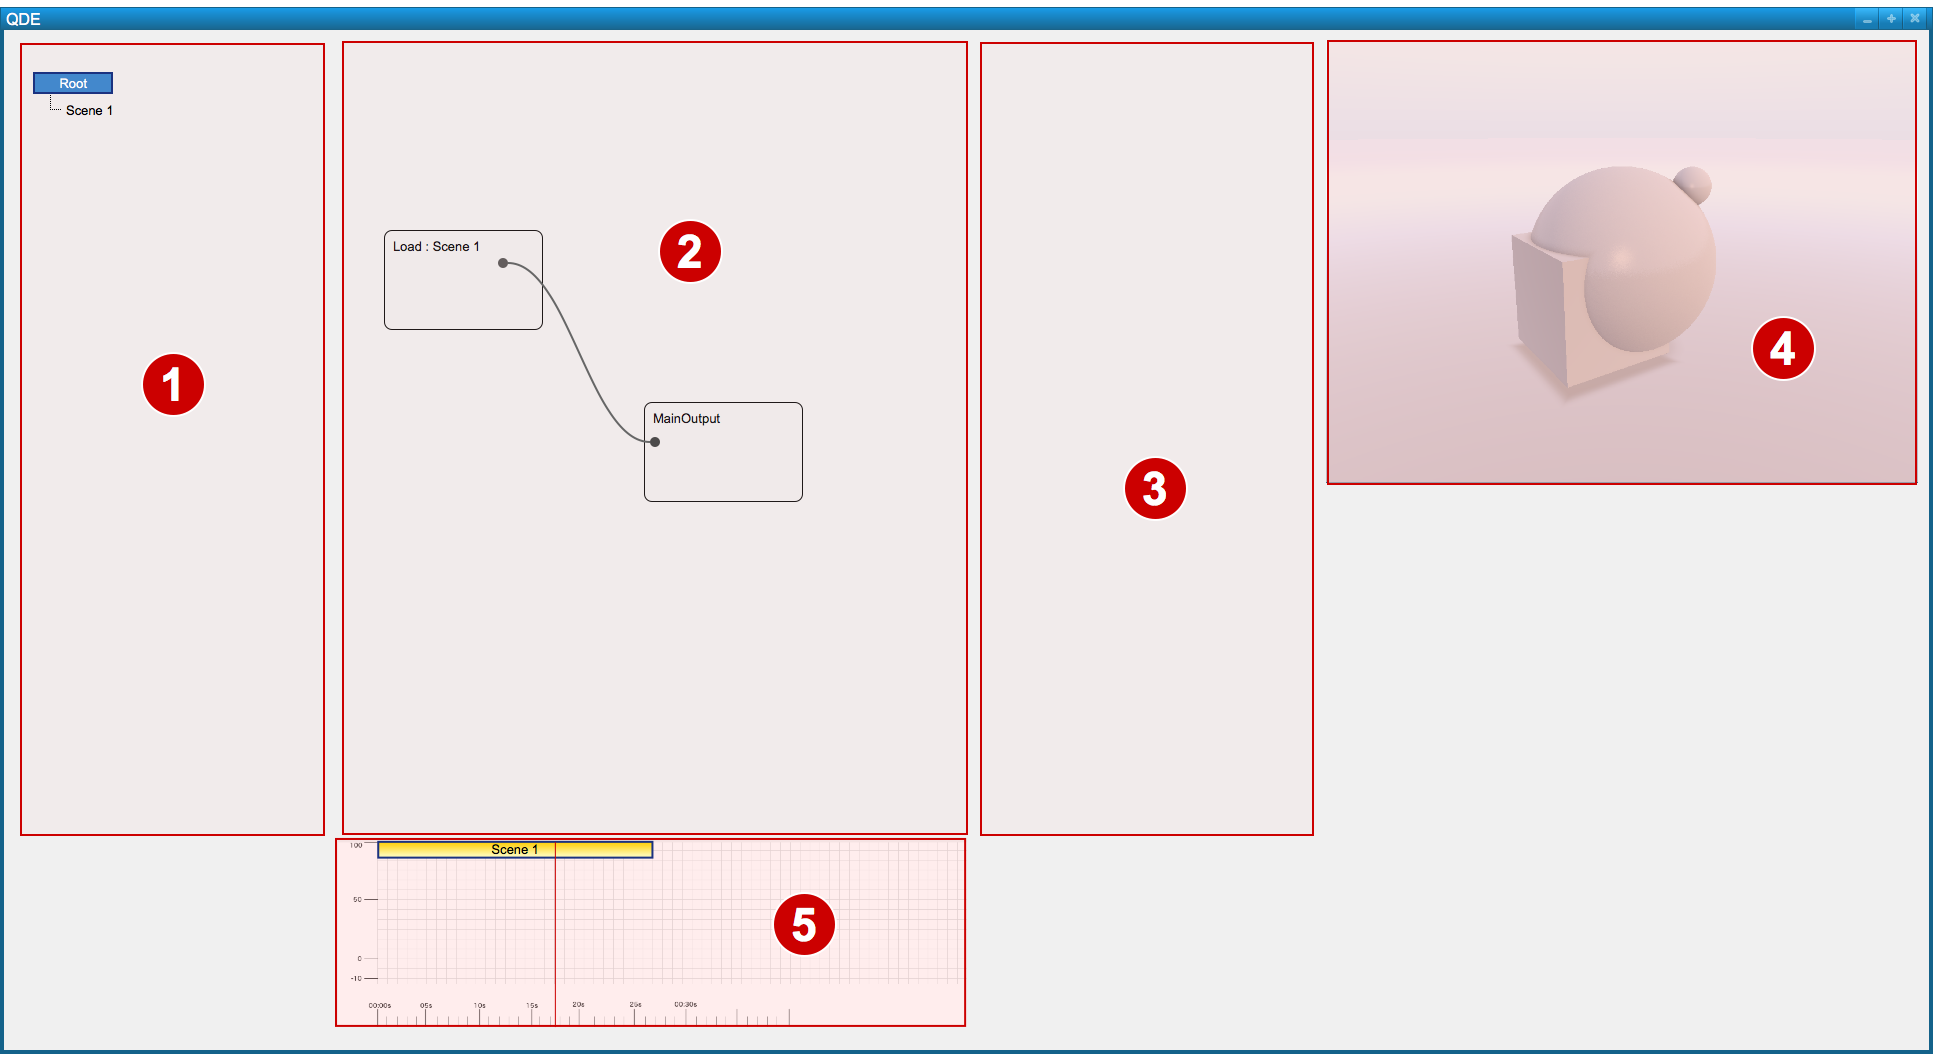
\includegraphics[width=0.95\linewidth]{images/editor-components}
\end{figure}

\newthought{Identifying the components} helps finding the noteworthy concepts or
objects. Decomposing a domain into noteworthy concepts or objects
is~\enquote{the quintessential object-oriented analysis
step}~\cite{larman-applying-2004}.~\enquote{The domain model is a visual
representation of conceptual classes or real-situation objects in a
domain.}~\cite{larman-applying-2004} The domain models for the editor and the
player component are shown in~\autoref{fig:editor-domain-model} and
in~\autoref{fig:player-domain-model} respectively.

\begin{figure*}[h]
  \caption{Domain model of the editor component.}
  \label{fig:editor-domain-model}
  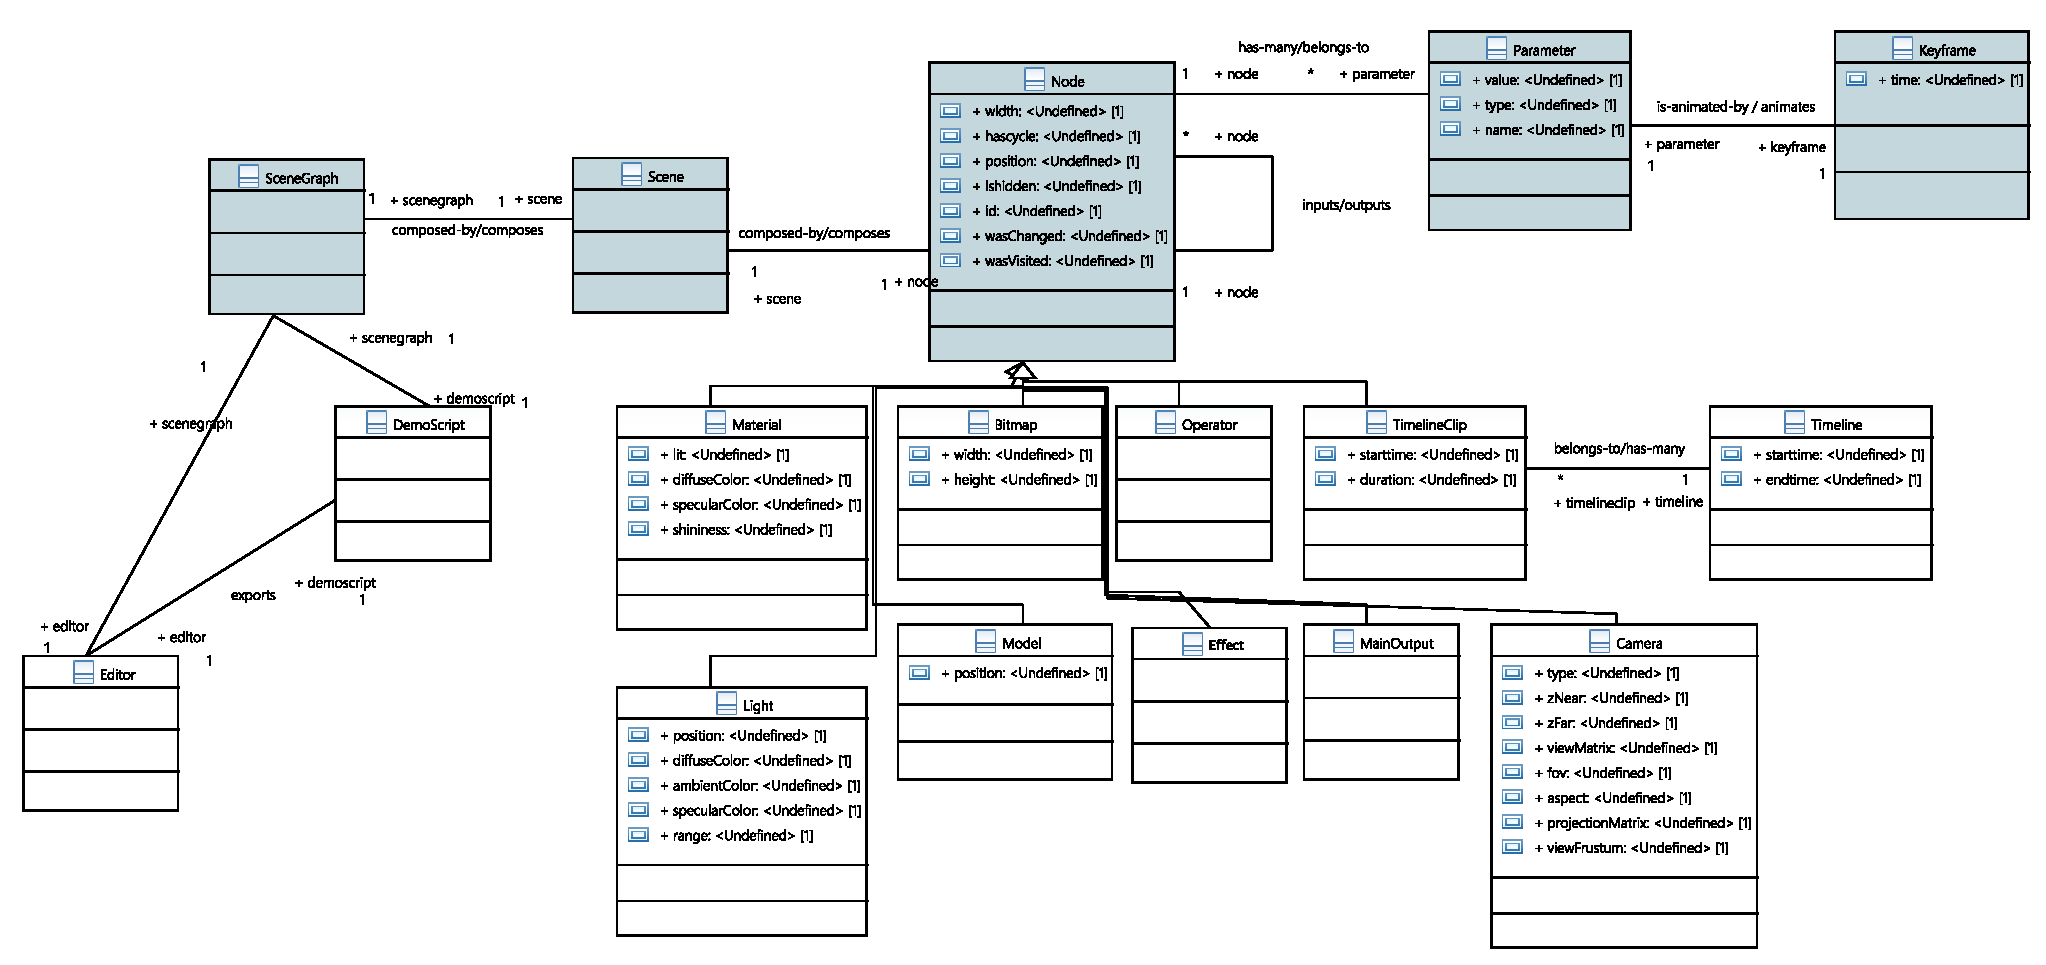
\includegraphics[width=0.95\linewidth]{images/editor-domain-model}
\end{figure*}

\begin{figure*}[ht]
  \caption{Domain model of the player component.}
  \label{fig:player-domain-model}
  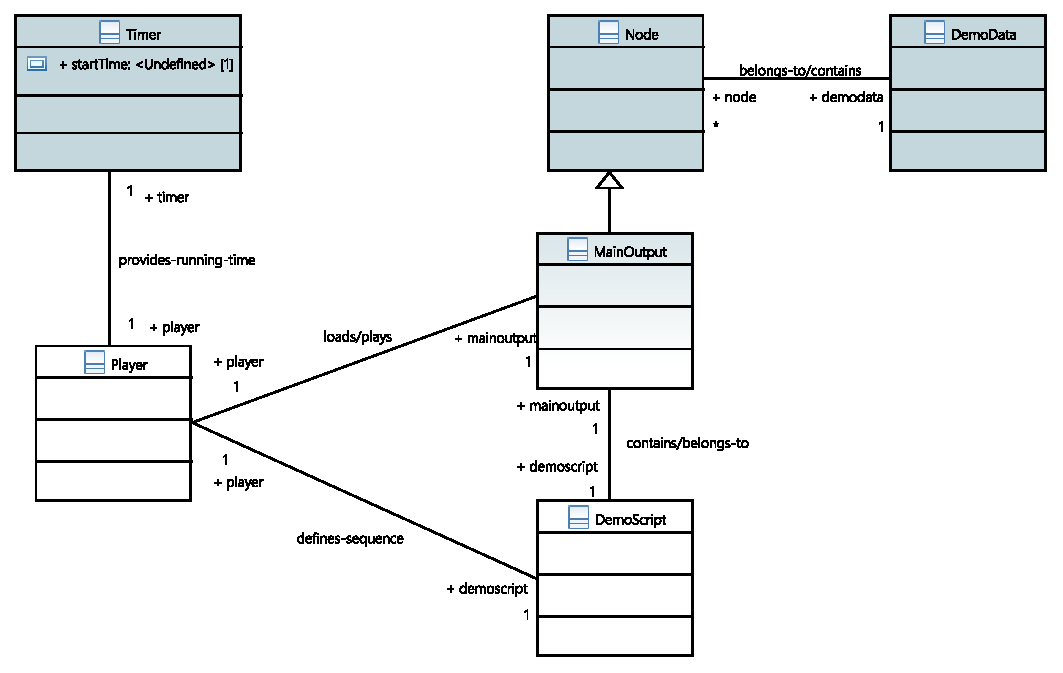
\includegraphics[width=0.95\linewidth]{images/player-domain-model}
\end{figure*}

% TODO: Add may be a reference to the documentation? The image of the editor
% domain model is too small to be read. --> Bigger, scaled and rotated. One
% figure per page.

\newthought{Identifying the noteworthy concepts or objects} allows the
definition of the logical architecture, which shows the overall image of
(software) classes in form of packets, subsystems and layers.

\newthought{To reduce coupling and dependencies} a relaxed layered architecture
is used. In contrast to a strict layered architecture, which allows any layer
calling only services or interfaces from the layer below, the relaxed layered
architecture allows higher layers to communicate with any lower layer. To ensure
low coupling and dependencies also for the graphical user interface, the models
and their views are segregated using the model-view separation principle. This
principle states that domain objects should have no direct knowledge about
objects of the graphical user interface. In addition controllers are used, which
represent workflow objects of the application layer.

\begin{table}[h]
  \caption{Layers of the envisaged software.}
  \label{table:layers}
  \begin{tabularx}{\textwidth}{lX}
    \toprule
    \textbf{Layer} & \textbf{Description}\\
    \midrule
    UI & All elements of the graphical user interface.\\
    Application & Controller/workflow objects.\\
    Domain & Models respectively logic of the application.\\
    Technical services & Technical infrastructure, such as graphics, window
    creation and so on.\\
    Foundation & Basic elements and low level services, such as a timer, arrays
    or other data classes.\\
    \bottomrule
  \end{tabularx}
\end{table}

\newthought{Class diagrams provide a software point of view} whereas domain
models provide rather a conceptual point of view. A class diagram shows classes,
interfaces and their relationships.~\autoref{fig:editor-class-diagram} shows the
class diagram of the editor component whereas~\autoref{fig:player-class-diagram}
shows the class diagram for the player component.

\begin{figure*}[ht]
  \caption{Class diagram of the editor component.}
  \label{fig:editor-class-diagram}
  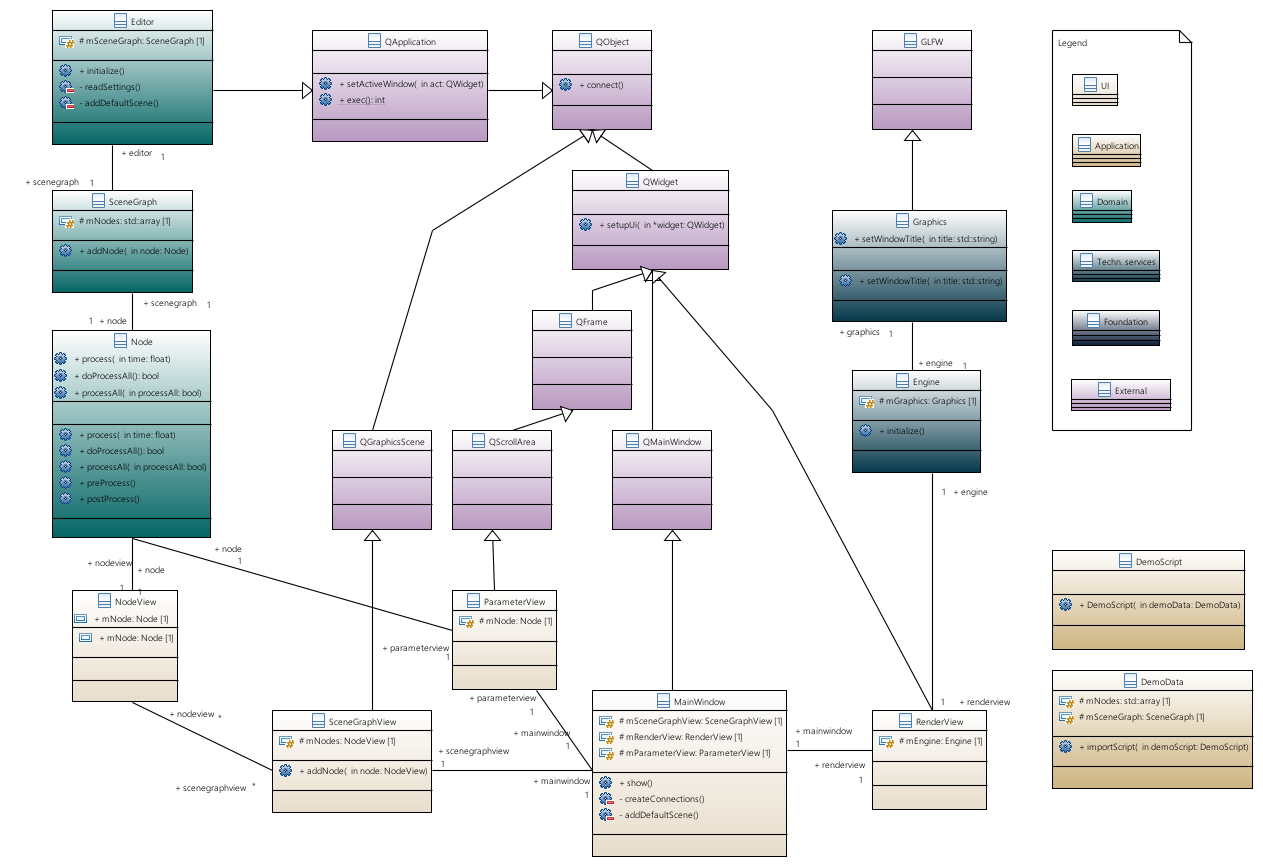
\includegraphics[width=0.95\linewidth]{images/editor-class-diagram}
\end{figure*}

\begin{figure*}[ht]
  \caption{Class diagram of the player component.}
  \label{fig:player-class-diagram}
  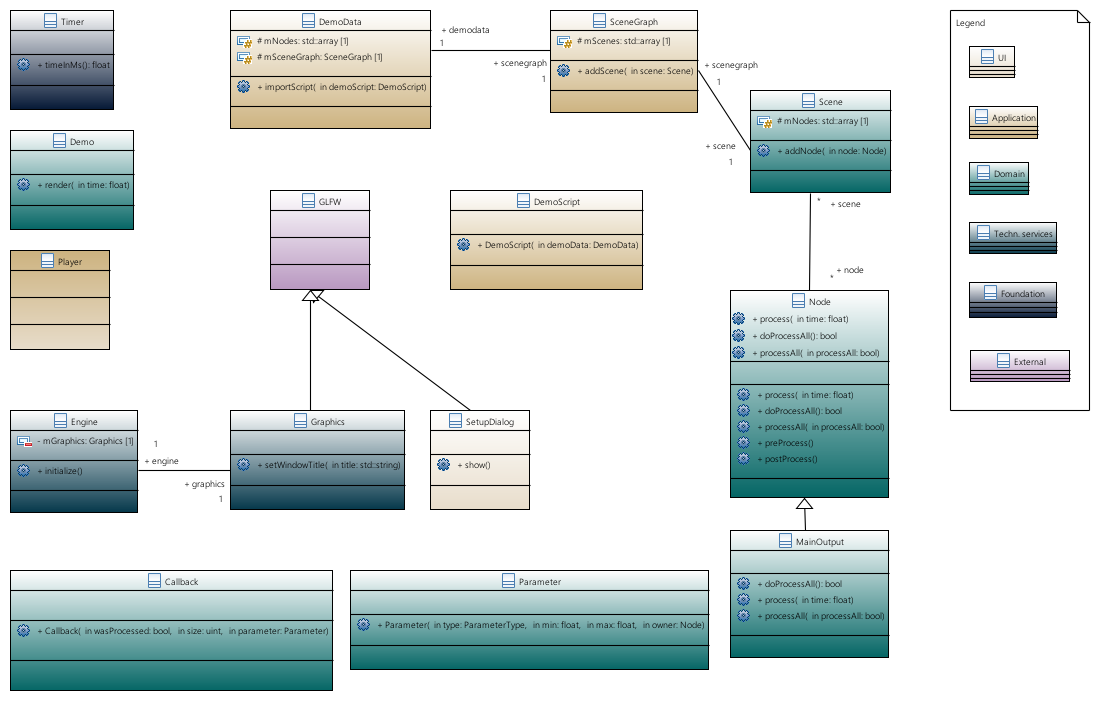
\includegraphics[width=0.95\linewidth]{images/player-class-diagram}
\end{figure*}

% TODO: Add may be a reference to the documentation? The images of the class
% diagrams are too small to be read. --> Bigger, scaled and rotated. One figure
% per page.

\section{Rendering}
\label{sec:rendering}

\newthought{This~\autoref{sec:rendering}} is a summary of a previous project
work of the author,~\enquote{Volume ray casting --- basics \&
principles}~\cite{osterwalder-volume-2016}. It describes the fundamentals for
the rendering algorithm that is used for the intended software of this thesis.

\newthought{Rendering} is one of the main aspects of this thesis, as the main
objective of the thesis is the design and development of a software for
modeling, composing and \textit{rendering} real time computer graphics through a
graphical user interface. \citeauthor{foley_computer_1996} describes rendering
as a~\enquote{process of creating images from
models}~\cite{foley_computer_1996}. The basic idea of rendering is to determine
the color of a surface at a certain point. For this task two concepts have
evolved: \textit{illumination models} and \textit{shading models}.
\newthought{Shading models} define when to use which illumination model and the
parameters for the illumination model.

\newthought{Illumination models} describe the amount of light that is
transmitted from a point on a surface to a viewer. There exist two kinds of
illumination models: local illumination models and global illumination models.
Whereas local illumination models aggregate local data from adjacent surfaces
and directly incoming light, global illumination models consider also indirect
light. The algorithm used for rendering in the intended software is an
algorithm using a \textit{global illumination model}.

\newthought{Global illumination models}~\enquote{express the light being
transferred from one point to another in terms of the intensity of the light
emitted from the first point to the second}~\cite[pp. 775 and
776]{foley_computer_1996}. Additionally to this direct intensity the indirect
intensity is considered, therefore ~\enquote{the intensity of light emitted from
all other points that reaches the first and is reflected from the first to the
second}~\cite[pp. 775 and 776]{foley_computer_1996} point is added.

\newpage{}

\newthought{In 1986 James~\enquote{Jim}~Kajiya} set up the so called rendering
equation, which expresses this behavior.~\parencites{kajiya_rendering_1986}[p.
776]{foley_computer_1996}

\begin{figure}
  \label{eq:rendering-equation}
  \caption{The rendering equation as defined by James~\enquote{Jim} Kajiya.}
  \begin{equation}
    I(x, x') = g(x, x')[\varepsilon(x, x') + \int\limits_{S}\rho(x, x', x'')I(x', x'')dx'']
  \end{equation}
\end{figure}

\marginnote{%-130pt
  \begin{description}
    \item[$x, x' \text{and } x''$] Points in space.
    \item[$I(x, x')$] Intensity of the light going from point $x'$ to point $x$.
    \item[$g(x, x')$] A geometrical term.
      \begin{description}
        \item[$0$] $x$ and $x'$ are occluded by each other.
        \item[$\frac{1}{r^2}$] $x$ and $x'$ are visible to one other, $r$ being
          the distance between the two points.
      \end{description}
    \item[$\varepsilon(x, x')$] Intensity of the light being emitted from point
      $x'$ to point $x$.
    \item[$\rho(x, x', x'')$] Intensity of the light going from $x''$ to $x$, being
      scattered on the surface of point $x'$.
    \item[$\int\limits_{S}$] Integral over the union of all surfaces, hence $S =
      \bigcup\limits_{i=0}^{n} S_{i}$, $n$ being the number of surfaces.
      All points $x$, $x'$ and $x''$ brush all surfaces of all objects within
      the scene. $S_{0}$ being an additional surface in form of a hemisphere
      which spans the whole scene and acts as background.
  \end{description}
}

% \begin{table}[h]
%   \caption{Description of the single aspects of the rendering equation.}
%   \begin{tabularx}{\textwidth}{lX}
%     \toprule
%     \textbf{Part} & \textbf{Description} \\
%     \midrule
%     $x, x' \text{and } x''$ & Points in space. \\
%     \midrule
%     $I(x, x')$ & Intensity of the light going from point $x'$ to point $x$. \\
%     \midrule
%     $g(x, x')$ & A geometrical term. \newline
%         \hspace*{4mm} $0$: \hspace*{2mm} $x$ and $x'$ are occluded by each other.
%         \newline
%         \hspace*{4mm} $1\over{r^2}$: \hspace*{1mm} $x$ and $x'$ are visible to one
%         other, $r$ being the \newline
%         \hspace*{12mm} distance between the two points. \\
%     \midrule
%     $\varepsilon(x, x')$ & Intensity of the light being emitted from point $x'$
%     to point $x$. \\
%     \midrule
%     $\rho(x, x', x'')$ & Intensity of the light going from $x''$ to $x$, being
%     scattered on the surface of point $x'$. \\
%     \midrule
%     $\int\limits_{S}$ & Integral over the union of all surfaces, hence $S =
%     \bigcup\limits_{i=0}^{n} S_{i}$, $n$ being the number of
%     surfaces.
%     All points $x$, $x'$ and $x''$ brush all surfaces of all objects within the
%     scene. $S_{0}$ being an additional surface in form of a hemisphere which
%     spans the whole scene and acts as background.\\
%     \bottomrule
%   \end{tabularx}
% \end{table}

\newthought{Implementing a global illumination model} or the rendering equation
directly for rendering images in viable or even real time is not really
feasible, even on modern hardware. The procedure is computationally complex and
very time demanding.

\newthought{A simplified approach} to implement global illumination models (or
the rendering equation) is ray tracing. Ray tracing is able to produce high
quality, realistic looking images. Although it is still demanding in terms of
time and computations, the time complexity is reasonable for producing still
images. For producing images in real time however, the procedure is still too
demanding. This is where a special form of ray tracing comes in.

\newthought{Sphere tracing} is a ray tracing approach for implicit surfaces
introduced in~\citeyear{hart_sphere_1994} by~\citeauthor{hart_sphere_1994} in
his work~\citetitle{hart_sphere_1994}~\cite{hart_sphere_1994}. 
Sphere tracing is faster than the classical ray tracing approaches in finding
intersections between rays and objects. In contrast to the classical ray tracing
approaches, the marching distance on rays is not defined by an absolute or a
relative distance, instead distance functions are used. The distance functions
are used to expand unbounding volumes (in this concrete case spheres, hence the
name) along rays.~\autoref{fig:sphere-tracing-1} illustrates this procedure.

\begin{figure}[h]
    \centering
    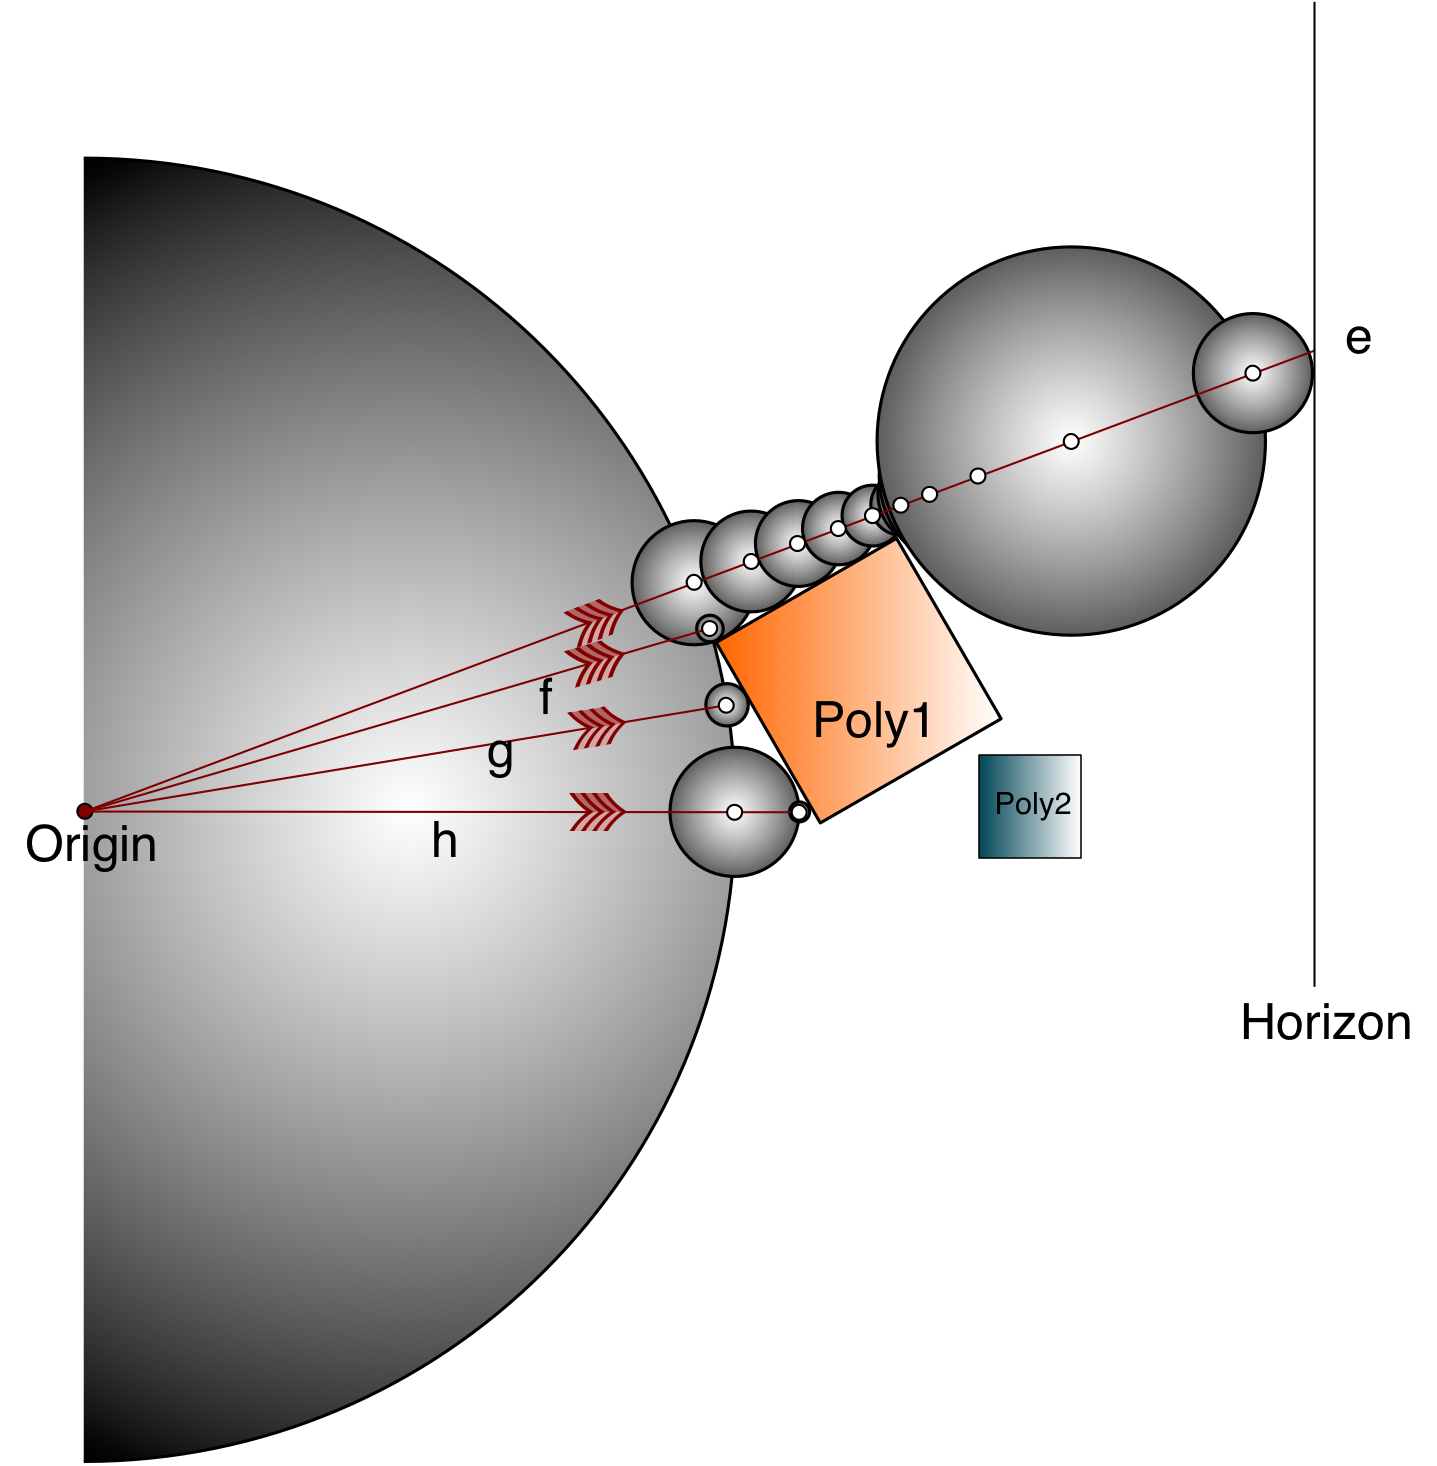
\includegraphics[width=0.75\linewidth]{images/sphere-tracing-principle}
    \caption{Illustration of the sphere tracing
      algorithm.
      Ray~\textit{e} hits no objects until reaching the horizon at
      $d_{max}$. Rays~\textit{f},~\textit{g} and~\textit{h} hit
      polygon~\textit{poly1}.}
      \label{fig:sphere-tracing-1}
\end{figure}

\newthought{Unbounding volumes} contrast with bounding volumes, which enclose a
solid. Unbounding volumes enclose a part of space without including certain
objects (whereas including means touching). For calculating a unbounding volume,
the distance between an object and the origin is being searched. Is this
distance known, it can be taken as a radius of a sphere. Sphere tracing defines
objects as implicit surfaces using distance functions. Therefore the distance
from every point in space to every other point in space and to every surface of
every object is known. These distances build a so called distance field.

\newthought{The sphere tracing algorithm} is as follows. A ray is being shot
from a viewer (an eye or a pinhole camera) through the image plane into a scene.
The radius of an unbounding volume in form of a sphere is being calculated at
the origin, as described above. This radius builds an intersection with the ray
and represents the distance, that the ray will travel in a first step. From this
intersection the next unbounding volume is being expanded and its radius is
being calculated, which gives the next intersection with the ray. This procedure
continues until an object is being hit or until a predefined maximum distance of
the ray $d_{max}$ is being reached. An object is being hit, whenever the
returned radius of the distance function is below a predefined constant
$\epsilon$. A possible implementation of the sphere tracing algorithm is shown
in~\autoref{alg:sphere-tracing}. This~\autoref{alg:sphere-tracing} is although
only showing the distance estimation. Shading is done outside, for example in a
render method which calls the sphere trace method. Shading means in this context
the determination of a surface's respectively a pixel's color.

 \begin{figure*}
   \label{alg:sphere-tracing}
   \caption{%
     An abstract implementation of the sphere tracing algorithm. Algorithm in
     pseudo code, after~\cite{hart_sphere_1994}[S. 531, Fig. 1]
   }
   \begin{pythoncode}
def sphere_trace():
    ray_distance          = 0
    estimated_distance    = 0
    max_distance          = 9001
    max_steps             = 100
    convergence_precision = 0.000001

    while ray_distance < max_distance:
        # sd_sphere is a signed distance function defining the implicit surface.
        # cast_ray defines the ray equation given the current traveled /
        # marched distance of the ray.
        estimated_distance = sd_sphere(cast_ray(ray_distance))

        if estimated_distance < convergence_precision:
            # the estimated distance is already smaller than the desired
            # precision of the convergence, so return the distance the ray has
            # travelled as we have an intersection
            return ray_distance

        ray_distance = ray_distance + estimated_distance

    # When we reach this point, there was no intersection between the ray and a
    # implicit surface, so simply return 0
    return 0
   \end{pythoncode}
\end{figure*}

\newthought{Shading} is done as proposed by~\citeauthor{whitted_improved_1980}
in~\citetitle{whitted_improved_1980}~\cite{whitted_improved_1980}. This means,
that the sphere tracing algorithm needs to return which object was hit and the
material of this object. Depending on the objects material, three cases can
occur:
\begin{enumerate*}
  \item the material is reflective and refractive,
  \item the material is only reflective or
  \item the material is diffuse.
\end{enumerate*}
For simplicity only the last case is being taken into account. For the actual
shading a local illumination method is used:~\textit{phong shading}.

\newthought{The phong illumination model} describes (reflected) light intensity
$I$ as a composition of the ambient, the diffuse and the perfect specular
reflection of a surface.

\begin{figure}
  \label{eq:phong-equation}
  \caption{The phong illumination model as defined by Phong Bui-Tuong. Note that
  the emissive term was left out intentionally as it is mainly used to achieve
  special effects.}
  \begin{equation}
    I(\vv{V}) = k_{a} \cdot L_{a} + k_{d} \displaystyle\sum_{i=0}^{n - 1} L_{i} \cdot (\vv{S_{i}} \cdot \vv{N}) + k_{s} \displaystyle\sum_{i=0}^{n - 1} L_{i} \cdot {(\vv{R_{i}} \cdot \vv{V})}^{k_{e}}
  \end{equation}
\end{figure}
% -*- mode: latex; coding: utf-8; outline-minor-mode: t -*-

\chapter{Methodologies}
\label{chap:methodologies}

% Das Kapitel der Methoden erklärt, was (Material) untersucht wurde und wie
% (Methode) ersteres untersucht wurde. Aufgrund der Beschreibung der Methoden muss
% es möglich sein, den Versuch oder die Studie zu wiederholen. Ist die
% Beschreibung der Versuchsanordnung oder des Vorgehens von sehr geringem Umfang,
% können diese nach Rücksprache mit der Betreuungsperson auch als Absatz in der
% Einleitung oder als Unterkapitel zum Kapitel der Einleitung verfasst werden.

% Link to previous
% Make a connection to what has immediately gone before. Recap the last chapter.
% In the last chapter I showed that… Having argued in the previous chapter that…
% As a result of x, which I established in the last chapter….. It is also possible
% to make a link between this chapter and the whole argument… The first step in
% answering my research question (repeat question) .. was to.. . In the last
% chapter I …
\newthought{The previous chapter} provided the fundamentals that are required for
understanding the results of this thesis.

% Focus: What does this chapter specifically do?
% Now focus the reader’s attention on what this chapter is specifically going to
% do and why it is important. In this chapter I will examine.. I will present… I
% will report … This is crucial in (aim of thesis/research question) in order to….
\newthought{This chapter} presents the methodologies that are used to implement
this thesis.

% Overview: How is it done?
% The third paragraph simply outlines the way that you are going to achieve the
% aim spelled out in the previous paragraph. It’s really just a statement of the
% contents in the order that the reader will encounter them. It is important to
% state these not simply as topics, but actually how they build up the internal
% chapter argument… I will begin by examining the definitions of, then move to
% seeing how these were applied… I first of all explain my orientation to the
% research process, positioning myself as a critical scholar.. I then explain the
% methodology that I used in the research, arguing that ethnography was the most
% suitable approach to provide answers to the question of…
\newthought{The first section of this chapter} shows a principle called literate
programming, which is used to generate this documentation and the practical
implementation in terms of a software. The second section describes the agile
methodologies, that are used to implement this thesis.

\section{Literate programming}
\label{sec:literate-programming}

\newthought{Software may be documented in different ways.} It may be in terms of
a preceding documentation, e.g. in form of a software architecture, which
describes the software conceptually and hints at its implementation. It may be
in terms of documenting the software inline through inline comments. Frequently
both methodologies are used, in independent order. However, all too frequently
the documentation is not done properly and is even neglected as it can be quite
costly with seemingly little benefit.

\newthought{Documenting software is crucial.} Whenever software is written,
decisions are made. In the moment a decision is made, it may seem intuitively
clear as it evolved by thought. This seemingly clearness of the decision is most
of the time deceptive. Is a decision still clear when some time has passed by
since making that decision? What were the facts that led to it? Is the decision
also clear for other, may be less involved persons? All these concerns show that
documenting software is crucial. No documentation at all, outdated or irrelevant
documentation can lead to unforeseen efforts concerning time and costs.

\newthought{\citeauthor{hoare-hpl-1973} states~\citeyear{hoare-hpl-1973}} in his
work~\citetitle{hoare-hpl-1973} that~\enquote{documentation must be regarded as
an integral part of the process of design and coding}~\cite[p.
195]{hoare-hpl-1973}: ~\enquote{The purpose of program documentation is to
explain to a human reader the way in which a program works so that it can be
successfully adapted after it goes into service, to meet the changing
requirements of its users, or to improve it in the light of increased knowledge,
or just to remove latent errors and oversights. The view that documentation is
something that is added to a program after it has been commissioned seems to be
wrong in principle and counter-productive in practice. Instead, documentation
must be regarded as an integral part of the process of design and coding. A good
programming language will encourage and assist the programmer to write clear
self-documenting code, and even perhaps to develop and display a pleasant style
of writing. The readability of programs is immeasurably more important than
their writeability.}~\cite[p. 195]{hoare-hpl-1973}

\newthought{Literate programming}, a paradigm proposed
in~\citeyear{knuth-lp-1984} by~\citeauthor{knuth-lp-1984}, goes even further.
\citeauthor{knuth-lp-1984} believes that \enquote{significantly better
documentation of programs} can be best achieved~\enquote{by considering programs
to be works of literature}~\cite[p.
1]{knuth-lp-1984}.~\citeauthor{knuth-lp-1984} proposes to change
the~\enquote{traditional attitude to the construction of programs}~\cite[p.
1]{knuth-lp-1984}. Instead of imagining that the main task is to instruct a
computer what to do, one shall concentrate on explaining to human beings what
the computer shall do.~\cite[p. 1]{knuth-lp-1984}

\newthought{The ideas of literate programming} have been embodied in several
software systems, the first being~\emph{WEB}, introduced
by~\citeauthor{knuth-lp-1984} himself. These systems are a combination of two
languages:
\begin{enumerate*}
  \item a document formatting language and
  \item a programming language
\end{enumerate*}.
Such a software system uses a single document as input (which can be split up in
multiple files) and generates two outputs:
\begin{enumerate*}
\item a document in a document formatting language, such as~\LaTeX{} which, may
    then be converted in a platform independent binary description, such as
    PDF.
  \item a compilable program in a programming language, such as Python or C
    which may then be compiled into an executable program.
\end{enumerate*}~\cite{knuth-lp-1984}
The first is called~\emph{weaving} and the latter~\emph{tangling}. This process
is illustrated in~\autoref{fig:weave-and-tangle}.

\begin{figure}
  \label{fig:weave-and-tangle}
  \caption{Illustration showing the processes of~\emph{weaving}
    and~\emph{tangling} documents from a input document.~\cite{knuth-lp-1984}}
  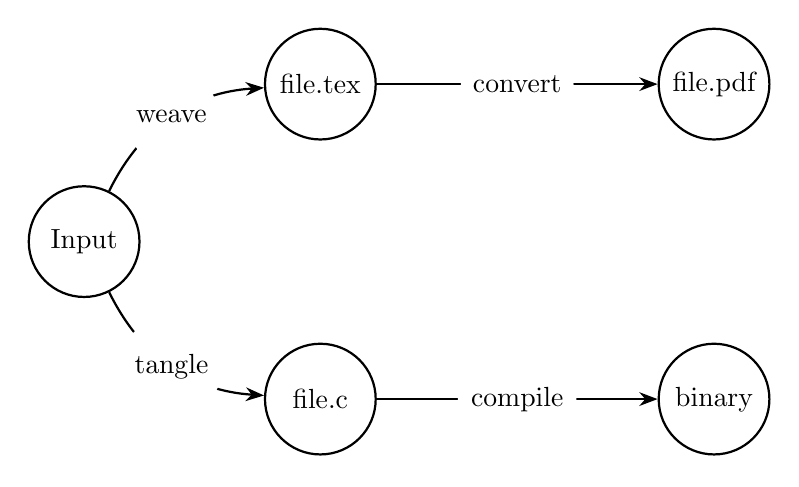
\begin{tikzpicture}
    \begin{scope}[every node/.style={minimum size=4em,circle,thick,draw}]
      \node (input) at (0,  0) {Input};
      \node (tex)   at (3,  2) {file.tex};
      \node (c)     at (3, -2) {file.c};
      \node (pdf)   at (8,  2) {file.pdf};
      \node (bin)   at (8, -2) {binary};
    \end{scope}
    \begin{scope}[>={Stealth[black]},
      every node/.style={fill=white,circle},
      every edge/.style={draw=black,thick}]
      \path [->] (input) edge[bend left=30] node {weave} (tex);
      \path [->] (input) edge[bend right=30] node {tangle} (c); 
      \path [->] (tex) edge node {convert} (pdf); 
      \path [->] (c) edge node {compile} (bin); 
    \end{scope}
  \end{tikzpicture}
\end{figure}

\newthought{Several literate programming systems were evaluated} during the
first phases of this thesis:
CWEB~\sidenote{\url{http://www-cs-faculty.stanford.edu/~uno/cweb.html}},
Noweb~\sidenote{\url{https://www.cs.tufts.edu/~nr/noweb/}},
lit~\sidenote{\url{http://cdosborn.github.io/lit/lit/root.html}},
PyLiterate~\sidenote{\url{https://github.com/bslatkin/pyliterate}},
pyWeb~\sidenote{\url{http://pywebtool.sourceforge.net/}} and
Babel~\sidenote{\url{http://orgmode.org/worg/org-contrib/babel/}} (which is part
of org mode of Emacs). All of these tools have their strengths and weaknesses.
However, none of these systems fulfill all the needed requirements:
\begin{enumerate*}
  \item Provide pretty printing of the program parts.
  \item Provide automatic references between the definition of program parts and
    their usage.
  \item Expand program parts having the same name instead of redefining them.
  \item Support Python as programming language.
  \item Allow the inclusion of files for both parts, the document formatting
    language and the programming language.
\end{enumerate*}

\newthought{Ultimately nuweb~\footnote{\url{http://nuweb.sourceforge.net/}} was
chosen} as it fulfills all these requirements. It has adapted and simplified the
ideas FunnelWeb~\footnote{\url{http://www.ross.net/funnelweb/}}. It is
independent of the programming language for the source code. As document
formatting language it uses~\LaTeX{}. Although the documentation of nuweb
states, that it has no pretty printing of source code, it provides an option to
display source code as listings. This method was modified to support visualizing
the expansion of parts as well as to use specific syntax highlighting and code
output within~\LaTeX{}.

\newthought{nuweb provides several commands to process files.} All commands
begin with an at sign (@). Whenever a file does not contain any commands the
file is copied unprocessed. The same applies for parts of files which contain no
commands. nuweb provides a single binary, which processes the
input files and generates the output files (in document formatting language and
as source code respectively). The commands are used to~\emph{specify output
files},~\emph{define fragments }and to~\emph{delimit scraps}.

\begin{table}[h]
  \caption{The major commands of nuweb.~\cite[p. 3]{briggs-nuweb-93}}
  \label{table:nuweb-commands}
  \begin{tabularx}{\textwidth}{lX}
    \toprule
    \textbf{Command} & \textbf{Description}\\
    \midrule
    \verb|@o file-name flags scrap| & \emph{Outputs} the given scrap to the
                                       defined \emph{file} using the provided
                                       flags.\\
    \verb|@d fragment-name scrap|   & Defines a~\emph{fragment} which refers to
                                       / holds the given scrap.\\
    \verb|@q fragment-name scrap|   & Defines a~\emph{quoted fragment} which refers to
                                       / holds the given scrap. Inside a quoted
                                       fragment referred fragments are not expanded.\\
    \bottomrule
  \end{tabularx}
\end{table}
\marginnote[-70pt]{Note that fragment names may be abbreviated, either during
invocation or definition. nuweb simply preserves the longest version of a
fragment name.~\cite[p. 4]{briggs-nuweb-93}}

\newthought{Scraps define content} in form of source code. They~\enquote{have
specific markers to allow precise control over the contents and
layout.}~\cite{briggs-nuweb-93} There are three ways of defining scraps, which
can be seen in~\autoref{table:nuweb-scraps}. They all include everything between
the specific markers but they differ when being typeset.
\begin{table}[h]
  \caption{Ways of defining scraps in nuweb.~\cite[p. 3]{briggs-nuweb-93}}
  \label{table:nuweb-scraps}
  \begin{tabularx}{\textwidth}{lX}
    \toprule
    \textbf{Scrap} & \textbf{Typesetting}\\
    \midrule
    \verb|@{ Content of scrap here @}| & Verbatim mode.\\
    \verb|@[ Content of scrap here @]| & Paragraph mode.\\
    \verb|@( Content of scrap here @)| & Math mode.\\
    \bottomrule
  \end{tabularx}
\end{table}

\newthought{A fragment is being invoked} by
using~\verb|@<fragment-name@>|.~\enquote{It causes the fragment fragment-name
to be expanded inline as the code is written out to a file. It is an error to
specify recursive fragment invocations.}~\cite[p. 3]{briggs-nuweb-93} There are
various other commands and details, but mentioning them would go beyond the
scope of this thesis. They can be found at~\cite{briggs-nuweb-93}.

\newthought{Literate programming can be very expressive} as all thoughts are
laid down before implementing something.~\citeauthor{knuth-lp-1984} sees this
expressiveness an advantage as one is forced to clarify his thoughts before
programming~\cite[p. 13]{knuth-lp-1984}. This is surely very true for rather
small software and partly also for larger software. The problem with larger
software is, that using literate programming, the documentation tends to be
rather large too. \emph{To overcome this aspect} the actual implementation of
the intended software is moved to the appendix~\todo{insert reference to
appendix here}.

\newthought{Another problematic aspect is the implementation of technical
details} such as imports for example or plain getter and setter methods, which
may recur and may often be very similar. While this might be interesting for
software developers or technically oriented readers, who want to grasp all the
details, this might not be interesting for other readers.~\emph{This aspect can
be overcome}, by moving recurring or seemingly uninteresting parts to a separate
file, see~\todo{add reference to code fragments}, which holds these code
fragments.

\newthought{To show the principles of literate programming} nevertheless,
without annoying the reader, only an excerpt of some details is given at this
place. One of the more interesting things of the intended software might
be the definition of a node~\todo{add reference to the node concept within
appendix} and the loading of node definitions from external files. These two
aspects are shown below. However, not all of the details are shown as this would
go beyond the scope.

\newthought{Some essential thoughts about classes and objects} may help to stay
consistent when developing the software, before implementing the node class.
Each class should at least have
\begin{enumerate}
  \item Signals --- to inform other components about events.
  \item A constructor.
  \item Various methods.
  \item Slots --- to get informed about events from other components.
\end{enumerate}
This pattern is applied to the declaration of the node class.

\newpage{}

\newthought{Implementing the node class} means simply defining a~\emph{scrap}
called~\enquote{\emph{Node definition declaration}} using the above pattern.
The~\emph{scrap} does not have any content at the moment, except references to
other scraps, which build the body of the scrap and which will be defined later
on.

\begin{figure}[h]
  \begin{flushleft} \small
\begin{minipage}{\linewidth}\label{scrap1}\raggedright\small
\NWtarget{nuweb?}{} $\langle\,${\itshape Node definition declaration}\nobreak\ {\footnotesize {?}}$\,\rangle\equiv$
\vspace{-1ex}
\begin{pythoncode}
class NodeDefinition(object):
    """Represents a definition of a node."""

    # Signals
    |\hbox{$\langle\,${\itshape Node definition signals}\nobreak\ {\footnotesize ?}$\,\rangle$}|
    |\hbox{$\langle\,${\itshape Node definition constructor}\nobreak\ {\footnotesize \NWlink{nuweb?}{?}}$\,\rangle$}|
    |\hbox{$\langle\,${\itshape Node definition methods}\nobreak\ {\footnotesize ?}$\,\rangle$}|

    # Slots
    |\hbox{$\langle\,${\itshape Node definition methods}\nobreak\ {\footnotesize ?}$\,\rangle$}||\NWsep|
\end{pythoncode}
\vspace{1.5ex}
\footnotesize
\begin{list}{}{\setlength{\itemsep}{-\parsep}\setlength{\itemindent}{-\leftmargin}}
\item {\NWtxtMacroNoRef}.

\item{}
\end{list}
\end{minipage}\vspace{4ex}
\end{flushleft}
\caption{Declaration of the node definition class.}
  \label{lst:node-def-class-decl}
\end{figure}

\vspace*{-2\baselineskip}
\newthought{The constructor} might be the first thing to implement, following
the developed pattern. In Python the constructor defines the properties of a
class~\sidenote[][-10pt]{Properties do not need to be defined in the constructor,
they may be defined anywhere within the class. However, this can lead to
confusion and it is therefore considered as good practice to define the
properties of a class in its constructor.}, therefore it defines what a class
actually is or represents --- the concept. After some thinking, and in context
of the intended software, one might come up with the properties
in~\autoref{table:node-properties} defining a node definition.

\begin{table*}[!htp]
  \begin{tabularx}{\linewidth}{lX}
    \toprule
    \textbf{Property} & \textbf{Description}\\
    \midrule
    ID          & A globally unique identifier for the node definition.          \\
    Name        & The name of the definition.                                    \\
    Description & The description of the definition. What does that definition
                  provide?                                                       \\
    Parent      & The parent object of the current node definition.              \\
    Inputs      & Inputs of the node definition. This may be distinct types or
                  references to other nodes.                                     \\
    Outputs     & The same as for inputs.                                        \\
    Invocation  & A list of the node's invocations or calls respectively.        \\
    Parts       & Defines parts that may be processed when evaluating the node.
                  Contains code which can be interpreted directly.               \\
    Connections & A list of connections of the node's inputs and outputs. Each
                  connection is composed by two parts:
                  \begin{enumerate*}
                    \item a reference to another node and
                    \item a reference to an input or an output of that node.
                  \end{enumerate*}
                  Is the reference not set, that is, its value is zero, this
                  means that the connection is internal.                         \\
    Instances   & A list of node instances from a certain node definition.       \\
    Was changed & Flag, which indicates whether a definition was changed or not. \\
    \bottomrule
  \vspace*{\baselineskip}
  \caption{Properties/attributes of the node class.}
  \label{table:node-properties}
  \end{tabularx}
\end{table*}

\newthought{Implementing the constructor} of the node definition may now follow
from the properties defined in~\autoref{table:node-properties}. As the name of
the constructor definition was already given, by using it
within~\autoref{lst:node-def-class-decl}
(\verb|@<Node definition constructor@>|), the very same name will be used for
actually defining the scrap itself.

\begin{figure}[!htbp]
  \begin{flushleft} \small
\begin{minipage}{\linewidth}\label{scrap2}\raggedright\small
\NWtarget{nuweb?}{} $\langle\,${\itshape Node definition constructor}\nobreak\ {\footnotesize {?}}$\,\rangle\equiv$
\vspace{-1ex}
\begin{pythoncode}
def __init__(self, id_):
    """Constructor.

    :param id_: the globally unique identifier of the node.
    :type  id_: uuid.uuid4
    """

    self.id_         = id_

    self.name        = ""
    self.description = ""
    self.parent      = None
    self.inputs      = []
    self.outputs     = []
    self.invocations = []
    self.parts       = []
    self.nodes       = []
    self.connections = []
    self.instances   = []
    self.was_changed = False|\NWsep|
\end{pythoncode}
\vspace{1.5ex}
\footnotesize
\begin{list}{}{\setlength{\itemsep}{-\parsep}\setlength{\itemindent}{-\leftmargin}}
\item \NWtxtMacroRefIn\ \NWlink{nuweb?}{?}.

\item{}
\end{list}
\end{minipage}\vspace{4ex}
\end{flushleft}
\caption{Constructor of the node definition class. Note that the
    identifier is given by a corresponding parameter. Identifiers have to be
    generated when defining a node using an external file.}
  \label{lst:node-def-constructor}
\end{figure}

\newthought{One of the problems mentioned before} can be seen
in~\cref{lst:node-def-constructor}: it shows a rather dull constructor without
any logic which is not interesting. Additionally importing of modules would be
needed, e.g. PyQt or system modules. This was left out deliberately. At this
point the implementation of node definitions will not be shown further, as this
is beyond scope. Further implementation can be seen at~\todo{insert
reference(s) to node domain model here}.

\newthought{Node definitions will be loaded from external files} in JSON format.
This happens within the node controller component, which will not be shown here
as this would go beyond the scope. Required attributes will be mentioned
explicitly although. The method for loading the nodes,
\mintinline{python}{load_node_definitions}, defined
in~\cref{lst:load-node-definitions}, does not have any arguments. Everything
needed for loading nodes is encapsulated in the node controller.

\begin{figure}[h]
  \begin{flushleft} \small
\begin{minipage}{\linewidth}\label{scrap3}\raggedright\small
\NWtarget{nuweb?}{} $\langle\,${\itshape Load node definitions}\nobreak\ {\footnotesize {?}}$\,\rangle\equiv$
\vspace{-1ex}
\begin{pythoncode}
def load_node_definitions(self):
    """Loads all files with the ending NODES_EXTENSION
    within the NODES_PATH directory, relative to
    the current working directory.
    """
|\NWsep|
\end{pythoncode}
\vspace{1.5ex}
\footnotesize
\begin{list}{}{\setlength{\itemsep}{-\parsep}\setlength{\itemindent}{-\leftmargin}}
\item \NWtxtMacroDefBy\ \NWlink{nuweb?}{?}\NWlink{nuweb?}{, ?}.
\item {\NWtxtMacroNoRef}.

\item{}
\end{list}
\end{minipage}\vspace{4ex}
\end{flushleft}
\caption{Head of the method that loads node definitions from external JSON
    files.}
  \label{lst:load-node-definitions}
\end{figure}

\vspace*{-2\baselineskip}
\newthought{When loading the node definitions}, there are two cases (and
consequences) at the first instance:
\begin{enumerate*}
  \item the directory containing the node definitions exists, the load
    definitions may be loaded or
  \item the directory does not exit.
\end{enumerate*}
In the first case the directory possibly containing node definitions is being
searched for such files, in the second case a warning message is logged.

\begin{figure}[!h]
  \begin{flushleft} \small
\begin{minipage}{\linewidth}\label{scrap4}\raggedright\small
\NWtarget{nuweb?}{} $\langle\,${\itshape Load node definitions}\nobreak\ {\footnotesize {?}}$\,\rangle+\equiv$
\vspace{-1ex}
\begin{pythoncode}
if os.path.exists(self.nodes_path):
    |\hbox{$\langle\,${\itshape Find and load node definition files}\nobreak\ {\footnotesize \NWlink{nuweb?}{?}, \ldots\ }$\,\rangle$}|
else:
    |\hbox{$\langle\,${\itshape Output warning when directory with node definitions does not exist}\nobreak\ {\footnotesize \NWlink{nuweb?}{?}}$\,\rangle$}||\NWsep|
\end{pythoncode}
\vspace{1.5ex}
\footnotesize
\begin{list}{}{\setlength{\itemsep}{-\parsep}\setlength{\itemindent}{-\leftmargin}}
\item \NWtxtMacroDefBy\ \NWlink{nuweb?}{?}\NWlink{nuweb?}{, ?}.
\item {\NWtxtMacroNoRef}.

\item{}
\end{list}
\end{minipage}\vspace{4ex}
\end{flushleft}
\caption{Check whether the path containing the node definition files exist or
    not.}
  \label{lst:nodes-controller-load-nodes-2}
\end{figure}

\vspace*{-2\baselineskip}
\newthought{In the first case}, when the directory containing the node
definitions exists, files containing node definitions are searched. The files
are searched by wildcard pattern matching the extension:~\verb|*.node|.

\begin{figure}[!h]
  \begin{flushleft} \small
\begin{minipage}{\linewidth}\label{scrap5}\raggedright\small
\NWtarget{nuweb?}{} $\langle\,${\itshape Find and load node definition files}\nobreak\ {\footnotesize {?}}$\,\rangle\equiv$
\vspace{-1ex}
\begin{pythoncode}
node_definition_files = glob.glob("{path}{sep}*.{ext}".format(
    path=self.nodes_path,
    sep=os.sep,
    ext=self.nodes_extension
))
num_node_definitions = len(node_definition_files)|\NWsep|
\end{pythoncode}
\vspace{1.5ex}
\footnotesize
\begin{list}{}{\setlength{\itemsep}{-\parsep}\setlength{\itemindent}{-\leftmargin}}
\item \NWtxtMacroDefBy\ \NWlink{nuweb?}{?}\NWlink{nuweb?}{, ?}.
\item \NWtxtMacroRefIn\ \NWlink{nuweb?}{?}.

\item{}
\end{list}
\end{minipage}\vspace{4ex}
\end{flushleft}
\caption{When the directory containing the node definitions exists, files
    matching the pattern~\emph{*.node} are searched.}
  \label{lst:nodes-controller-find-node-def-files}
\end{figure}

\vspace*{-2\baselineskip}
\newthought{Having searched for node definition files}, there are again two
cases, similar as before:
\begin{enumerate*}
  \item files (possibly) containing node definitions exist or
  \item no files with the ending \verb|.node| exist within the source directory.
\end{enumerate*}
Again, as before, in the first case the node definitions will be loaded, in the
second case a warning message will be logged.

\begin{figure}[!h]
  \begin{flushleft} \small
\begin{minipage}{\linewidth}\label{scrap6}\raggedright\small
\NWtarget{nuweb?}{} $\langle\,${\itshape Find and load node definition files}\nobreak\ {\footnotesize {?}}$\,\rangle+\equiv$
\vspace{-1ex}
\begin{pythoncode}
if num_node_definitions > 0:
    |\hbox{$\langle\,${\itshape Load found node definitions}\nobreak\ {\footnotesize \NWlink{nuweb?}{?}, \ldots\ }$\,\rangle$}|
else:
    |\hbox{$\langle\,${\itshape Output warning when no node definitions are found}\nobreak\ {\footnotesize \NWlink{nuweb?}{?}}$\,\rangle$}||\NWsep|
\end{pythoncode}
\vspace{1.5ex}
\footnotesize
\begin{list}{}{\setlength{\itemsep}{-\parsep}\setlength{\itemindent}{-\leftmargin}}
\item \NWtxtMacroDefBy\ \NWlink{nuweb?}{?}\NWlink{nuweb?}{, ?}.
\item \NWtxtMacroRefIn\ \NWlink{nuweb?}{?}.

\item{}
\end{list}
\end{minipage}\vspace{4ex}
\end{flushleft}
\caption{When files (possibly) containing node definition files are found,
    they are tried being loaded. When no such files are found, a warning message
    is being logged.}
  \label{lst:nodes-controller-find-node-def-files-2}
\end{figure}

\newthought{Given that node definitions are present}, they are loaded from the
file system, parsed and then stored internally as domain model. To maintain
readability, all this is encapsulated in a
method,\\
\mintinline{python}{load_node_definition_from_file_name}, which is
deliberately not\\
shown here as this would go beyond scope. If the node
definition cannot be loaded or parsed~\mintinline{python}{None} is being
returned.

\begin{figure}[!h]
  \begin{flushleft} \small
\begin{minipage}{\linewidth}\label{scrap7}\raggedright\small
\NWtarget{nuweb?}{} $\langle\,${\itshape Load found node definitions}\nobreak\ {\footnotesize {?}}$\,\rangle\equiv$
\vspace{-1ex}
\begin{pythoncode}
self.logger.info(
    "Found %d node definition(s), loading.",
    num_node_definitions
)
t0 = time.perf_counter()
for file_name in node_definition_files:
    self.logger.debug(
        "Found node definition %s, trying to load",
        file_name
    )
    node_definition = self.load_node_definition_from_file_name(
        file_name
    )|\NWsep|
\end{pythoncode}
\vspace{1.5ex}
\footnotesize
\begin{list}{}{\setlength{\itemsep}{-\parsep}\setlength{\itemindent}{-\leftmargin}}
\item \NWtxtMacroDefBy\ \NWlink{nuweb?}{?}\NWlink{nuweb?}{, ?}.
\item \NWtxtMacroRefIn\ \NWlink{nuweb?}{?}.

\item{}
\end{list}
\end{minipage}\vspace{4ex}
\end{flushleft}
\caption{Loading and parsing of the node definitions found within the folder
    containing (possibly) node definition files. If a node definition cannot be
    loaded or parsed,~\textit{None} is being returned.}
  \label{lst:nodes-controller-load-node-defs}
\end{figure}

\newpage{}

\newthought{When a node definition could be loaded}, a view model based on the
domain model is being created. Both models are then stored internally and a
signal about the loaded node definition is being emitted, to inform other
components which are interested in this event.

\begin{figure}[!h]
  \begin{flushleft} \small
\begin{minipage}{\linewidth}\label{scrap8}\raggedright\small
\NWtarget{nuweb?}{} $\langle\,${\itshape Load found node definitions}\nobreak\ {\footnotesize {?}}$\,\rangle+\equiv$
\vspace{-1ex}
\begin{pythoncode}
    if node_definition is not None:
        node_definition_view_model = node_view_model.NodeViewModel(
            id_=node_definition.id_,
            domain_object=node_definition
        )
        self.node_definitions[node_definition.id_] = (
            node_definition,
            node_definition_view_model
        )
        |\hbox{$\langle\,${\itshape Node controller load node definition emit}\nobreak\ {\footnotesize ?}$\,\rangle$}|

t1 = time.perf_counter()
self.logger.info(
    "Loading node definitions took %.10f seconds",
    (t1 - t0)
)|\NWsep|
\end{pythoncode}
\vspace{1.5ex}
\footnotesize
\begin{list}{}{\setlength{\itemsep}{-\parsep}\setlength{\itemindent}{-\leftmargin}}
\item \NWtxtMacroDefBy\ \NWlink{nuweb?}{?}\NWlink{nuweb?}{, ?}.
\item \NWtxtMacroRefIn\ \NWlink{nuweb?}{?}.

\item{}
\end{list}
\end{minipage}\vspace{4ex}
\end{flushleft}
\caption{A view model, based on the domain model, for the node definition is
    being created. Both models are then stored internally and the signal, that a
    node definition was loaded is being emitted.}
  \label{lst:nodes-controller-load-node-defs-2}
\end{figure}

\newpage{}

\newthought{The implementation of the edge cases} is still remaining at this
point. When such an edge case happens, a corresponding message is logged. The
edge cases are:

\begin{enumerate}
  \item the directory holding the node definitions does not exist
\end{enumerate}

\begin{figure}[!h]
  \begin{flushleft} \small
\begin{minipage}{\linewidth}\label{scrap9}\raggedright\small
\NWtarget{nuweb?}{} $\langle\,${\itshape Output warning when directory with node definitions does not exist}\nobreak\ {\footnotesize {?}}$\,\rangle\equiv$
\vspace{-1ex}
\begin{pythoncode}
    message = QtCore.QCoreApplication.translate(
        __class__.__name__,
        "The directory holding the node definitions, %s, does not exist." % self.nodes_path
    )
    self.logger.fatal(message)|\NWsep|
\end{pythoncode}
\vspace{1.5ex}
\footnotesize
\begin{list}{}{\setlength{\itemsep}{-\parsep}\setlength{\itemindent}{-\leftmargin}}
\item \NWtxtMacroRefIn\ \NWlink{nuweb?}{?}.

\item{}
\end{list}
\end{minipage}\vspace{4ex}
\end{flushleft}
\caption{Output a warning when the path containing the node definition files
    does not exist.}
  \label{lst:nodes-controller-load-node-defs-warning}
\end{figure}

\tuftebreak{}or

\begin{enumerate}[resume]
  \item no files containing node definitions are found.
\end{enumerate}
  
\begin{figure}[!h]
  \begin{flushleft} \small
\begin{minipage}{\linewidth}\label{scrap10}\raggedright\small
\NWtarget{nuweb?}{} $\langle\,${\itshape Output warning when no node definitions are found}\nobreak\ {\footnotesize {?}}$\,\rangle\equiv$
\vspace{-1ex}
\begin{pythoncode}
    message = QtCore.QCoreApplication.translate(
        __class__.__name__,
        "No files with node definitions found at %s." % self.nodes_path
    )
    self.logger.fatal(message)|\NWsep|
\end{pythoncode}
\vspace{1.5ex}
\footnotesize
\begin{list}{}{\setlength{\itemsep}{-\parsep}\setlength{\itemindent}{-\leftmargin}}
\item \NWtxtMacroRefIn\ \NWlink{nuweb?}{?}.

\item{}
\end{list}
\end{minipage}\vspace{4ex}
\end{flushleft}
\caption{Output a warning when no node definitions are being found.}
  \label{lst:nodes-controller-load-node-defs-warning-2}
\end{figure}

\section{Agile software development}
\label{sec:agile-software-development}

\newthought{Software engineering invokes always a methodology,} be it wittingly
or unwittingly. For a (very) small project the methodology may follow intuitively,
by experience and it may be a mixture of methodologies. For medium to large
projects however, using certain methodologies or principles becomes inevitable
for being able to evaluate (the success of) a project.

\newthought{Every commonly used software engineering methodology} has advantages
but buries also certain risks. Be it a traditional method like the waterfall
model, incremental development, the v-model, the spiral model or a more recent
method like agile development. It depends largely on the project what
methodology fits best and buries the least risks.~\cite{haneen-risk-2012,
mens-se-2008}

\newthought{Risk is the basic problem of software
development.}~\cite{beck-xp-2004} Examples of risks are: schedule slips,
canceled projects, increased defect rates, misunderstood domain/business,
changes, false feature rich.~\cite{beck-xp-2004}

\newthought{Traditional software engineering methodologies}, such as the
waterfall model or incremental development, struggle with change. In case of the
waterfall model they embrace change not at all or, in the case of incremental
development, the phases are rather long what allows only slow reaction.

\begin{figure*}[ht]
  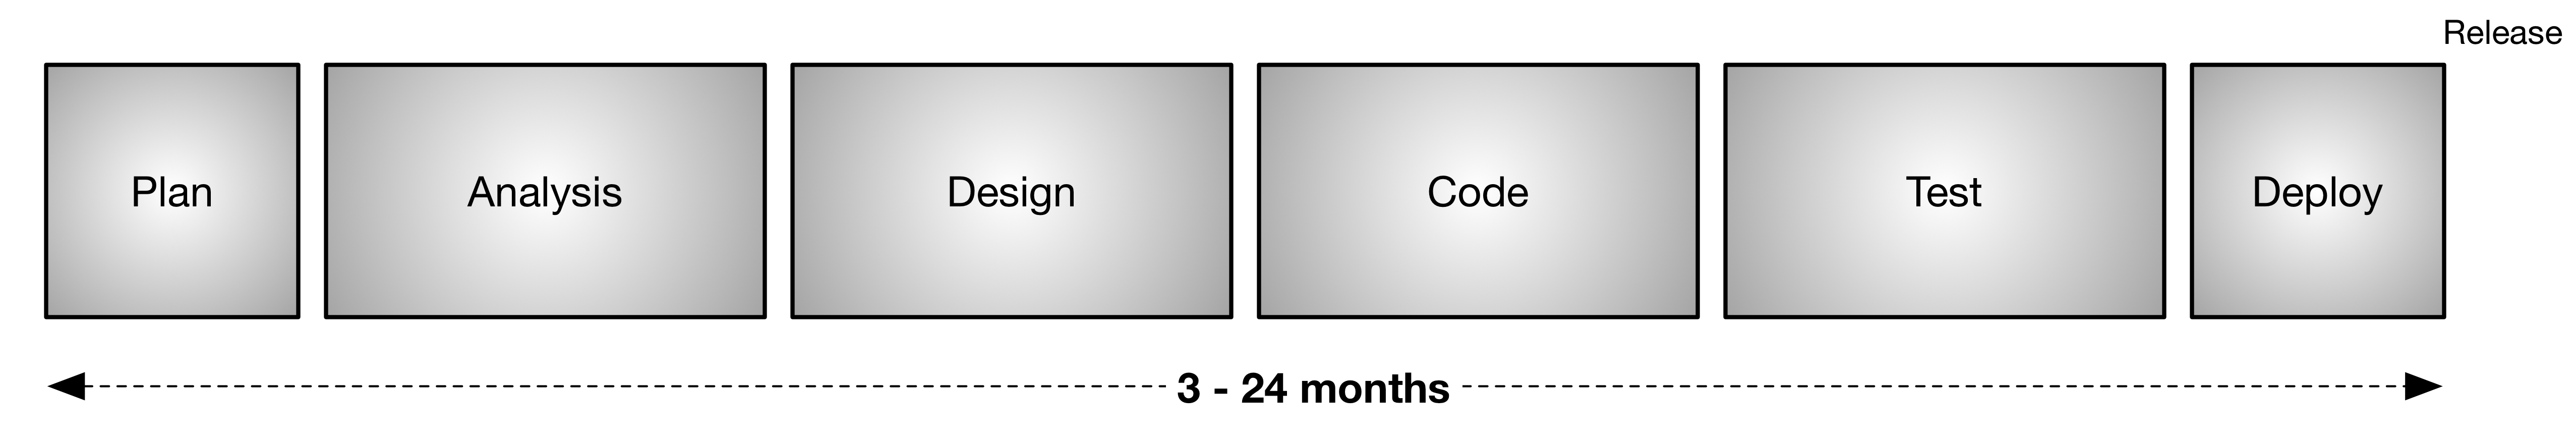
\includegraphics[width=0.95\linewidth]{images/waterfall}
  \caption{Phases of the water fall methodology.~\cite[p. 16]{shore-aad-2007}}
  \label{fig:waterfall}
\end{figure*}

\begin{figure*}[ht]
  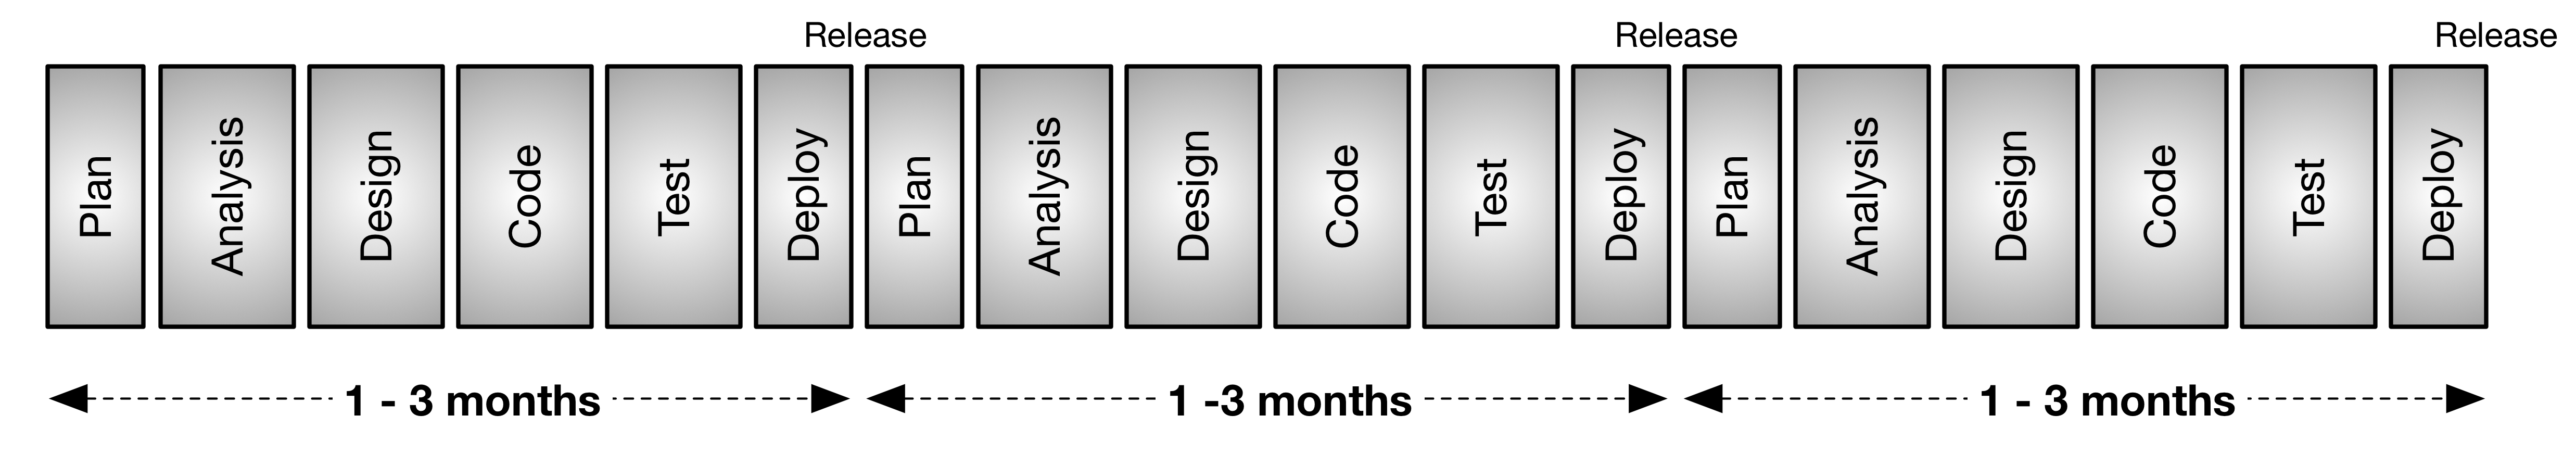
\includegraphics[width=0.95\linewidth]{images/iterative-dev}
  \caption{Phases of iterative development.~\cite[p. 16]{shore-aad-2007}}
  \label{fig:iterative-dev}
\end{figure*}

\newthought{By applying basic principles}, agile development methodologies try
to overcome this problem. These principles may vary depending on the used
methodology, but the fundamental principles are:
\begin{enumerate*}
  \item rapid feedback,
  \item assume simplicity,
  \item incremental change,
  \item embracing change and
  \item quality work.
\end{enumerate*}~\cite{beck-xp-2004}
Further details can be found at~\cite{beck-xp-2004, shore-aad-2007}.

\newthought{An adapted version of extreme programming} is used for this thesis.
This methodology was chosen as after the preceding project
work,~\citetitle{osterwalder-qde-2016}, several things were still subject to
change and therefore an exact planning, analysis and design, as traditional
methodologies require it, would not be very practical.
% TODO: Mention what exactly was modified.

\begin{figure*}[ht]
  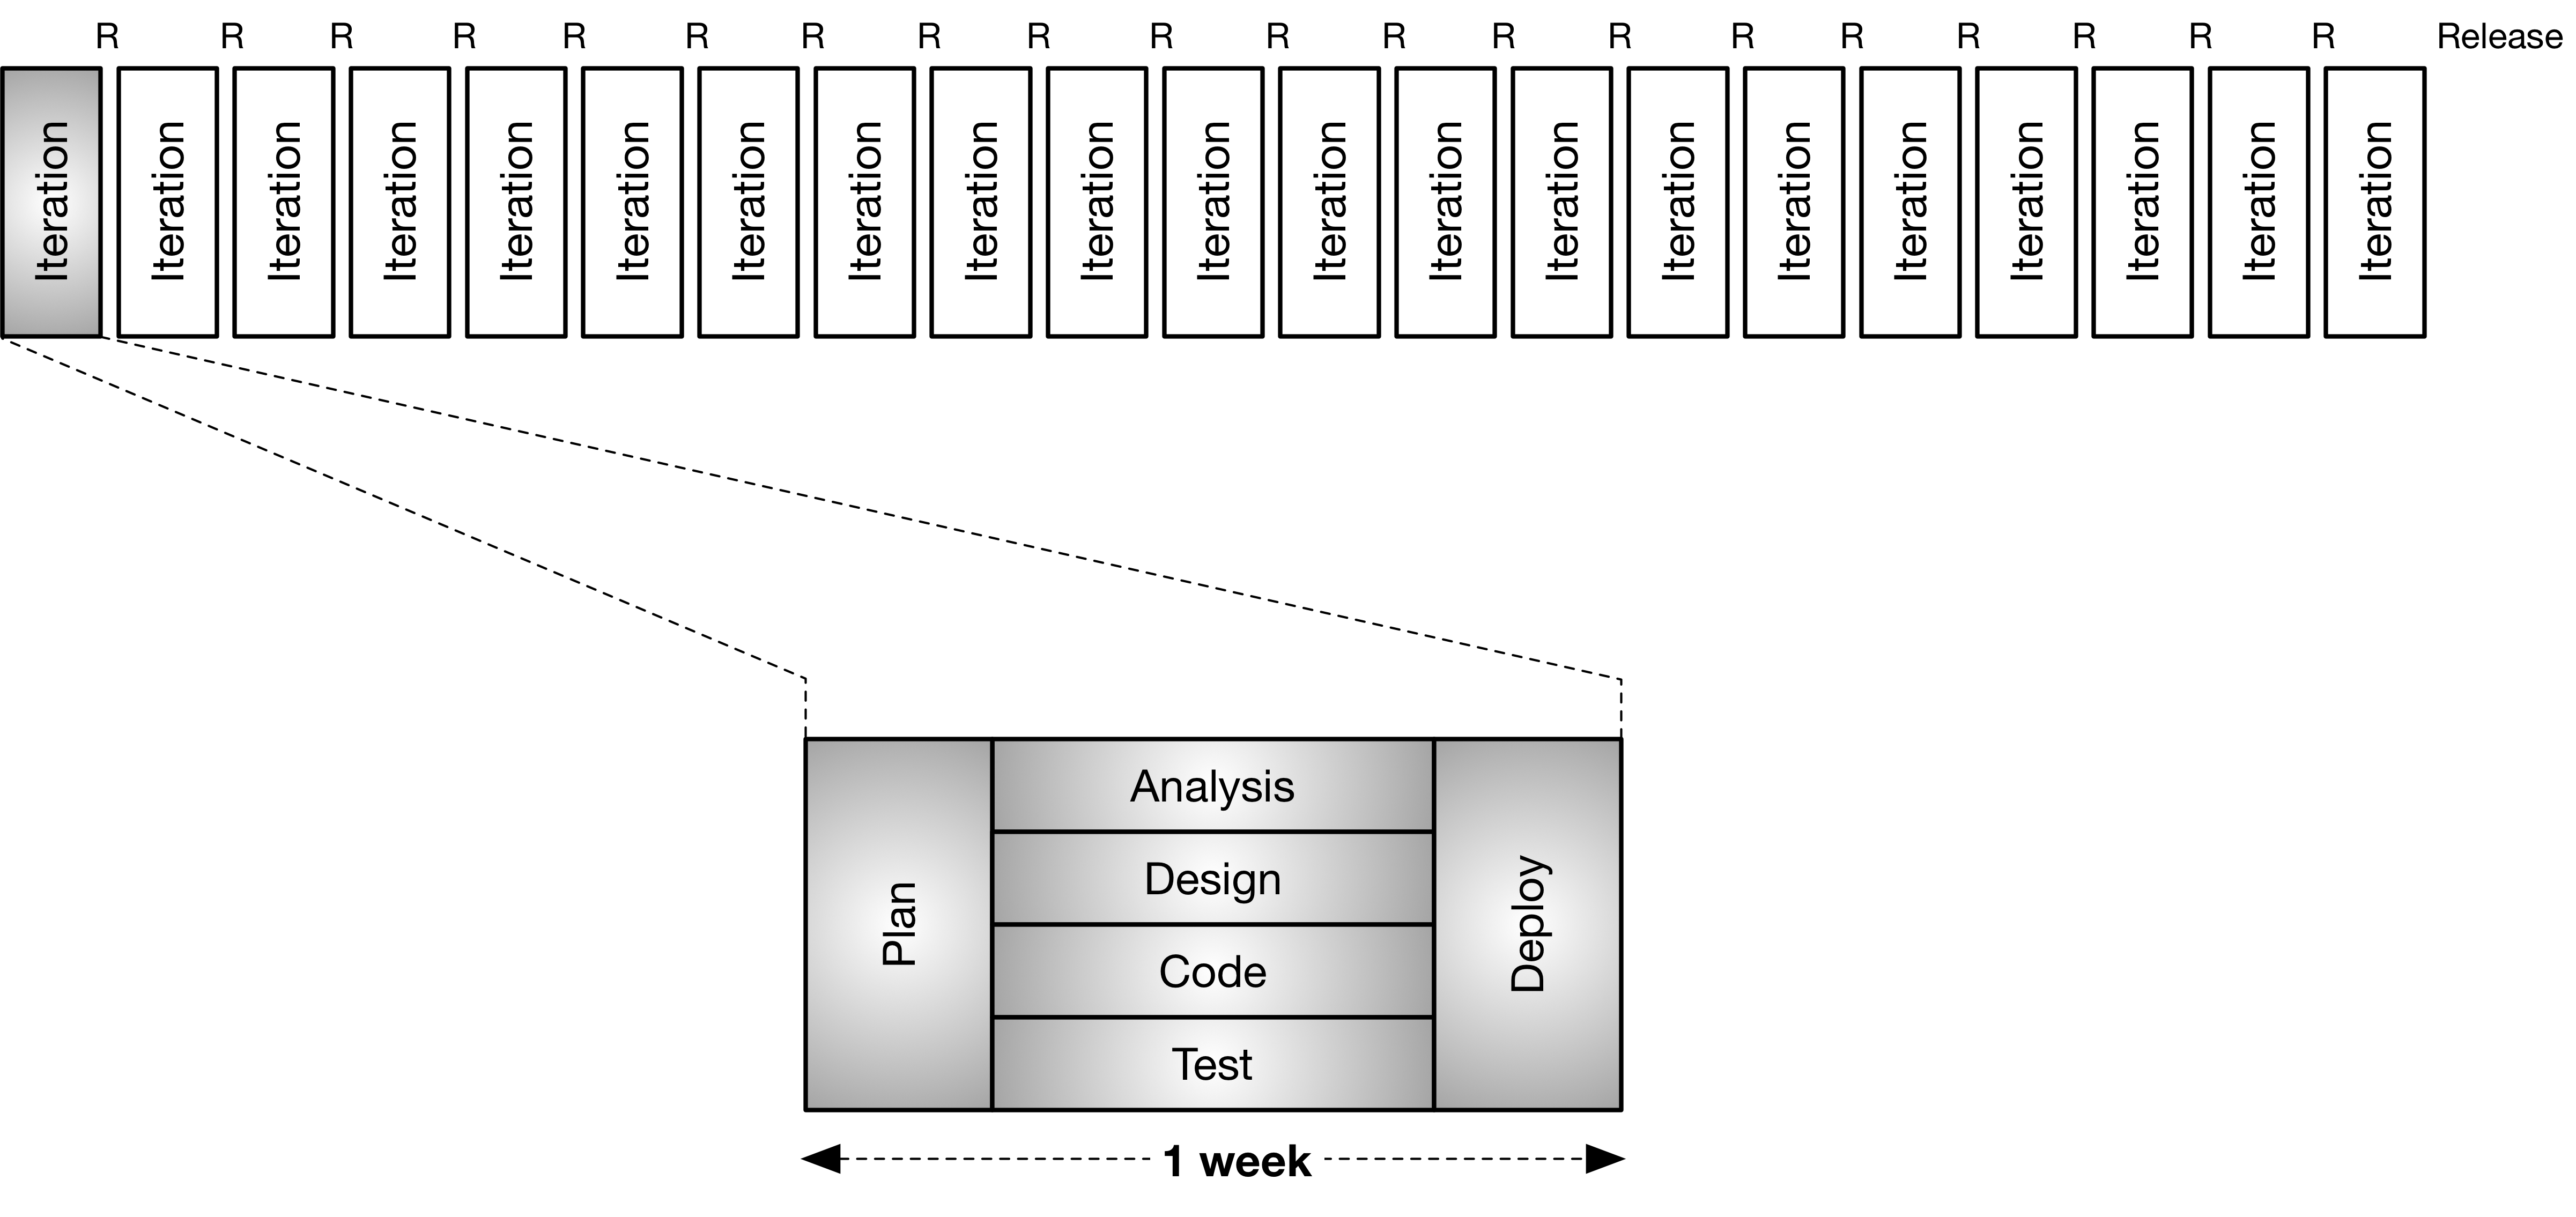
\includegraphics[width=0.95\linewidth]{images/xp}
  \caption{Iterations in the extreme programming methodology and phases of an
    interation.~\cite[p. 18]{shore-aad-2007}}
  \label{fig:xp}
\end{figure*}

% TODO: Check if this is enough or elaborate more otherwise.
% -*- mode: latex; coding: utf-8 -*-

\chapter{Implementation}
\label{chap:implementation}

% Gestützt auf Quellen, Messungen und Datenerhebungen werden die anhand der
% Fragestellung gewon- nenen Ergebnisse präsentiert [3, p. 116]. Während das
% Kapitel zu Material und Methoden ( 3.2.3) oder das entsprechende Unterkapitel
% der Einleitung die Versuchsanordnung beschreibt, werden im Kapitel Ergebnisse
% der Versuchsablauf mit den Resultaten objektiv wiedergegeben. Alle Überlegungen,
% Berechnungen oder Experimente des Berichts müssen vollständig nachvollziehbar
% sein [3, p. 26]. Zusammen mit der Diskussion und den Folgerungen machen die
% Ergebnisse qualitativ und quantitativ den Hauptteil des Berichts aus [3, p. 26].

% Link to previous
% Make a connection to what has immediately gone before. Recap the last chapter.
% In the last chapter I showed that… Having argued in the previous chapter that…
% As a result of x, which I established in the last chapter….. It is also possible
% to make a link between this chapter and the whole argument… The first step in
% answering my research question (repeat question) .. was to.. . In the last
% chapter I …
\newthought{The previous chapter} introduced the methodologies that are required
for understanding the following results of this thesis.

% Focus: What does this chapter specifically do?
% Now focus the reader’s attention on what this chapter is specifically going to
% do and why it is important. In this chapter I will examine.. I will present… I
% will report … This is crucial in (aim of thesis/research question) in order to….
\newthought{This chapter} presents the achieved results by means of three
sections. The first section shows the software architecture, that was developed
and that is used for the developed software. Aspects of the developed literate
program are shown in the second section. The main concepts and the components of
the developed software are shown in the third section.

% Overview: How is it done?
% The third paragraph simply outlines the way that you are going to achieve the
% aim spelled out in the previous paragraph. It’s really just a statement of the
% contents in the order that the reader will encounter them. It is important to
% state these not simply as topics, but actually how they build up the internal
% chapter argument… I will begin by examining the definitions of, then move to
% seeing how these were applied… I first of all explain my orientation to the
% research process, positioning myself as a critical scholar.. I then explain the
% methodology that I used in the research, arguing that ethnography was the most
% suitable approach to provide answers to the question of…
% * Software architecture
% ** Reference to actual chapter
% ** Layers
% ** Signals
%
% * Literate programming
% ** Just mention, reference to actual chapter
%
% * Software
% ** Editor
% ** Player
% ** Components
%
% Nope, merged this already with focus.

% Input CF
% Resultate weniger kritisch, erst in Diskussion, überlappt sich aber.

\section{Software architecture}
\label{results:sec:software-architecture}

\newthought{The software architecture} holds the significant decisions of the
envisaged software, the selection of structural elements, their behavior and
their interfaces.~\cite{kruchten_rup_2003} It is derived from the experiences
based on the former project works,~\citetitle{osterwalder-volume-2016}
and~\citetitle{osterwalder-qde-2016}, which are condensed to build the
fundamentals, see~\ref{chap:fundamentals}.

\newthought{Three aspects} define the software architecture:
\begin{enumerate*}
  \item an architectural software design pattern,
  \item layers and
  \item signals, allowing communication between components.
\end{enumerate*}

\subsection{Software design}
\label{results:subsec:software-design}

\newthought{A [software] design pattern}~\enquote{names, abstracts, and
identifies the key aspects of a common design structure that make it useful for
creating a reusable object-oriented design. The design pattern identifies the
participating classes and instances, their roles and collaborations, and the
distribution of responsibilities. Each design pattern focuses on a particular
object-oriented design problem or issue. It describes when it applies, whether
it can be applied in view of other design constraints, and the consequences and
trade-offs of its use.}~\cite[p. 16]{gamma-dpe-1995}

\newthought{To separate data from its representation} and to ensure a coherent
design, a combination of the model-view-controller (MVC) and the model-view-view
model pattern (MVVM) is used as architectural software design
pattern.~\cite{fowler-presentation-2004, gossman-mvvm-2005} This decision is
based on experiences from the previous project works and allows to modify and
reuse individual parts. This is especially necessary as the data created in the
editor component will be reused by the player component.

\newthought{Four kinds of components} build the basis of the used
pattern.~\cref{table:software-design-pattern-components} provides a description
of the components.~\cref{fig:software-design-pattern-components} shows an
overview of the components (the colored items) including their communication.
Additionally the user as well as the display is shown (in gray color).

\begin{table*}[h]
  \begin{tabularx}{\textwidth}{llX}
    \toprule
    \textbf{Component} & \textbf{Description} & \textbf{Examples} \\
    \midrule
    Model      & Represents the data or the business logic, & Scene, Node
                                                              Parameter\\
               & completely independent from the user       & \\
               & interface. It stores the state and does    & \\
               & the processing of the problem domain.      & \\
    \midrule
    View       & Consists of the visual elements.           & Scene graph view,
                                                              Scene view\\
    \midrule
    View model & \enquote{Model of a view}, abstraction of  & Scene graph view
                                                              model, Scene\\
               & the view, provides a specialization of the & view model, Node
                                                              view model\\
               & model that the view can use for            & \\
               & data-binding, stores the state and may     & \\
               & provide complex operations.                & \\
    \midrule
    Controller & Holds the data in terms of models.         & Scene graph
                                                              controller, scene
                                                              controller,\\
               & models. Acts as an interface between the   & node controller\\
               & components.                                & \\
    \bottomrule
  \end{tabularx}
  \caption{Description of the components of the used software design
    pattern.~\cite{fowler-presentation-2004, gossman-mvvm-2005}}
  \label{table:software-design-pattern-components}
\end{table*}

\begin{figure*}[ht]
  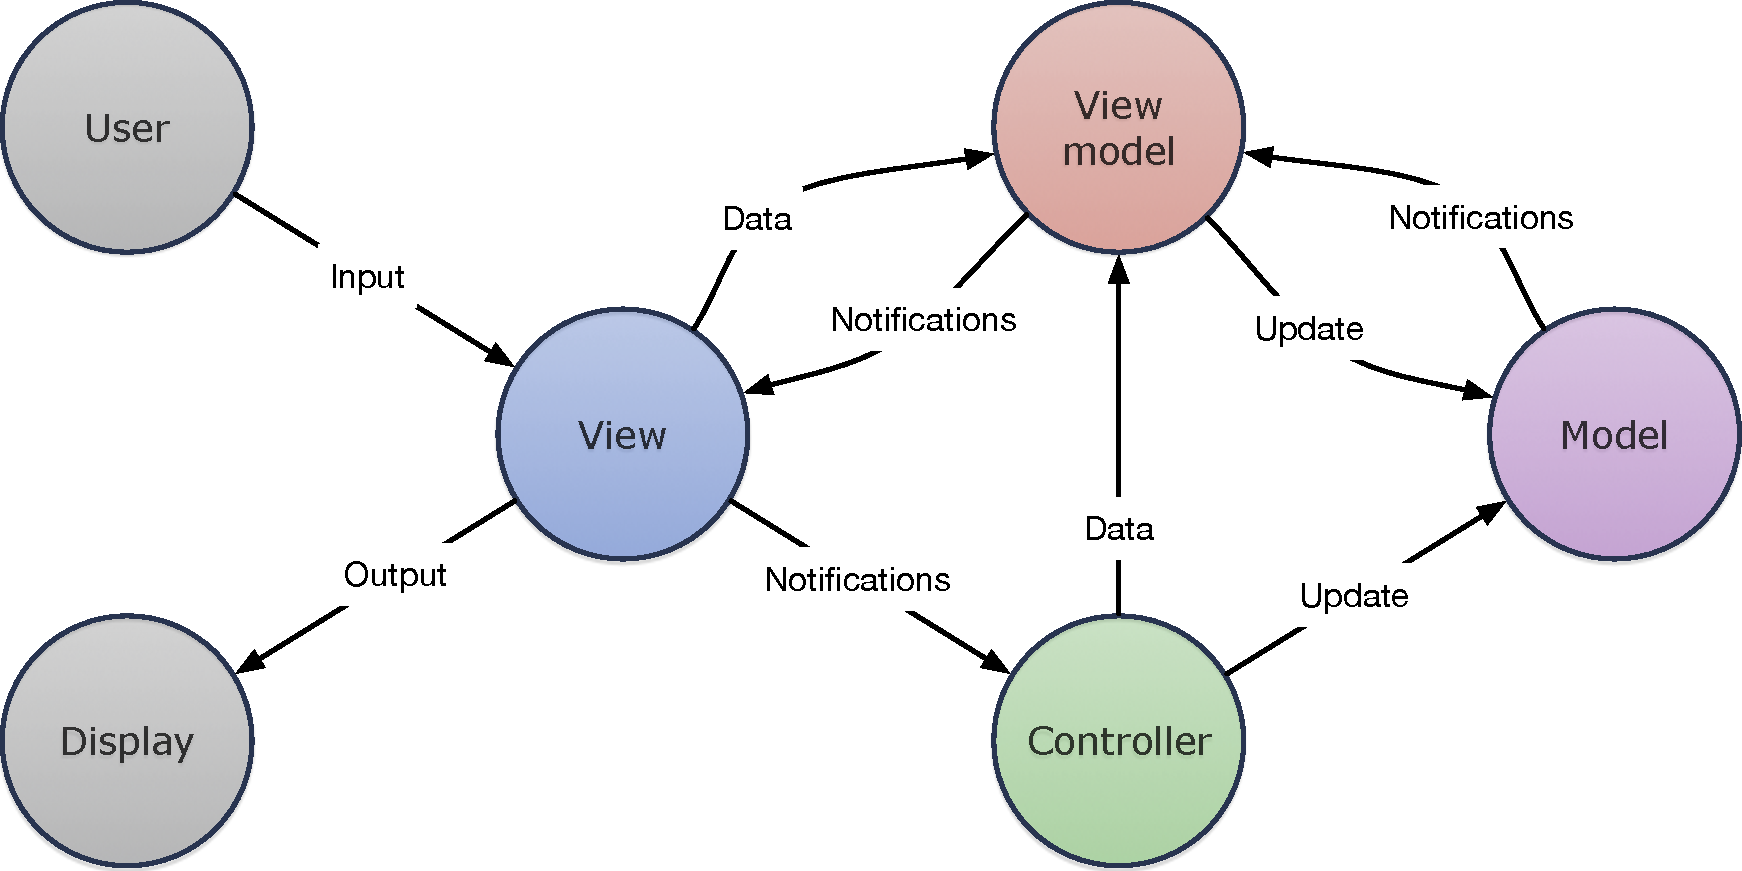
\includegraphics[width=0.8\linewidth]{images/mvvmc}
  \caption{Components of the used pattern and their communication.}
  \label{fig:software-design-pattern-components}
\end{figure*}

% Reference Qt's view model and explain why it was not used.
\newthought{The used Qt framework} provides a very similar pattern respectively
concept called~\enquote{model/view pattern}. It combines the view and the
controller into a single object. The pattern introduces a delegate between view
and model, similar to a view model. The delegate allows editing the model and
communicates with the view. The communication is done by so called model indices
coming from the model. Model indices are references to items of
data.~\cite{qt-mvp-2017}~\enquote{By supplying model indexes to the model, the
view can retrieve items of data from the data source. In standard views, a
delegate renders the items of data. When an item is edited, the delegate
communicates with the model directly using model indexes.}~\cite{qt-mvp-2017}
\cref{fig:software-design-pattern-qt-mvp} shows the model/view pattern.

\begin{figure}[ht]
  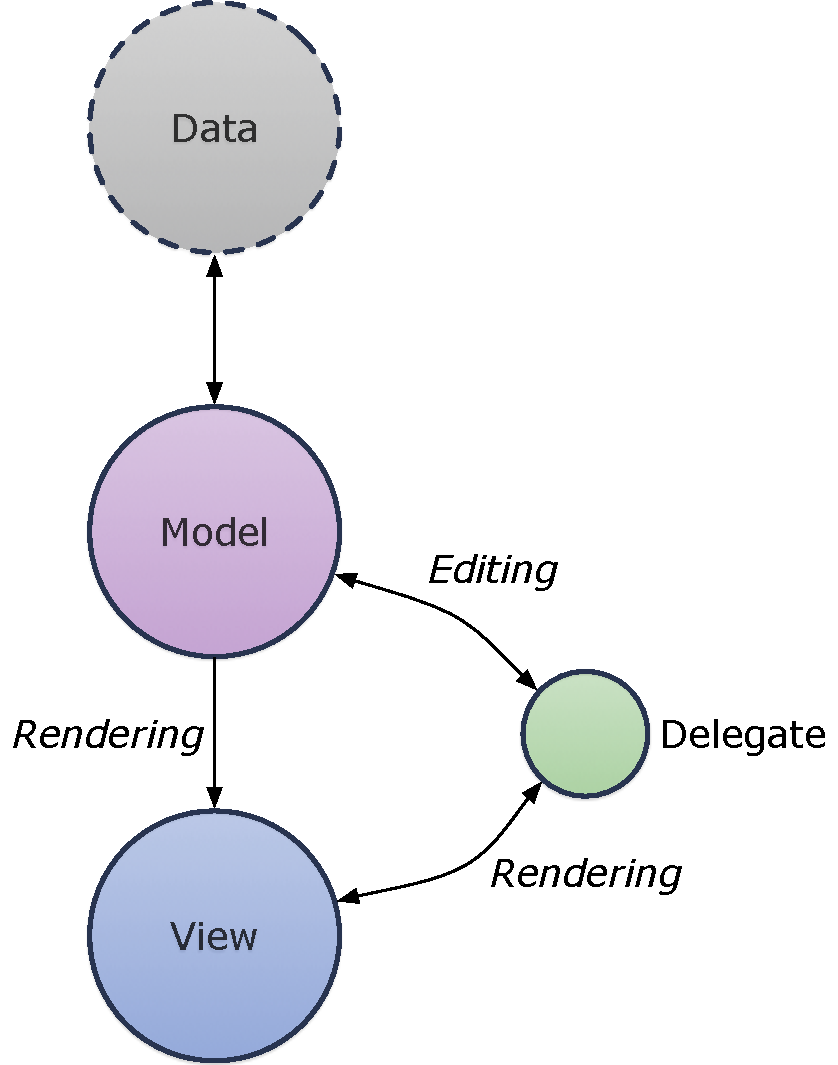
\includegraphics[width=0.6\linewidth]{images/model-view-pattern}
  \caption{Qt's model/view pattern.~\cite{qt-mvp-2017}}
  \label{fig:software-design-pattern-qt-mvp}
\end{figure}

\newthought{Although offering advantages}, such as to customize the presentation
of items or the usage of a wide range of data sources, the model/view pattern was
not used in general. This is mainly due to two reasons:
\begin{enumerate*}
  \item the developed and intended components use no data source except external
    files and
  \item the concept of using model indices may add flexibility but introduces
    also overhead.
\end{enumerate*} The scene graph component of the editor was developed using
Qt's abstract item model class which uses the model/view pattern. This showed,
that the usage of the pattern can introduce unnecessary overhead, in terms of
being more effort to implement, while not using the features of the pattern.
Therefore the decision was taken against the usage of the pattern.

\subsection{Layers}
\label{results:subsec:layers}

\newthought{To reduce coupling and dependencies} a relaxed layered architecture
is used, as written in~\cref{results:sec:software-architecture}. In contrast to a strict
layered architecture, which allows any layer calling only services or interfaces
from the layer below, the relaxed layered architecture allows higher layers to
communicate with any lower layer.~\cref{table:results:layers} provides a
graphical overview as well as a description of the layers. The colors have no
meaning except to distinguish the layers visually.

\begin{table*}[h]
  \begin{tabularx}{\textwidth}{XXX}
    \toprule
    \textbf{Layer} & \textbf{Description} & \textbf{Examples} \\
    \midrule
    
\includegraphics[width=1.0\linewidth]{images/layers-gui}         & All elements of the graphical user interface, views.                                  & Scene graph view, scene view, render view                                   \\
    
\includegraphics[width=1.0\linewidth]{images/layers-gui-domain}  & View models.                                                                          & Scene graph view model, node view model                                     \\
    
\includegraphics[width=1.0\linewidth]{images/layers-application} & Controller/workflow objects.                                                          & Main application, scene graph controller, scene controller, node controller \\
    
\includegraphics[width=1.0\linewidth]{images/layers-domain}      & Models respectively logic of the application.                                         & Scene model, parameter model, node definition model, node domain model      \\
    
\includegraphics[width=1.0\linewidth]{images/layers-technical}   & Technical infrastructure, such as graphics, window creation and so on.                & JSON parser, camera, culling, graphics, renderer                            \\
    
\includegraphics[width=1.0\linewidth]{images/layers-foundation}  & Basic elements and low level services, such as a timer, arrays or other data classes. & Colors, common, constants, flags                                            \\
    \bottomrule
  \end{tabularx}
  \vspace*{\baselineskip}
  \caption{Layers of the developed software.}
  \label{table:results:layers}
\end{table*}

\subsection{Signals and slots}
\label{results:subsec:signals}

% Signals:  Explain what signals are and how they are used, maybe draw an
% illustrative diagram.

\newthought{Whenever designing and developing} software, coupling and cohesion
can occur and may pose a problem if not considered early enough and properly.
\textit{Coupling} measures how strongly a component is connected, has knowledge
of or depends on other components. High coupling impedes the readability and
maintainability of software. Therefore low coupling ought to be strived.
\citeauthor{larman-applying-2004} states, that the principle of low coupling
applies to many dimensions of software development and that it is one of the
cardinal goals in building
software.~\cite{larman-applying-2004}~\textit{Cohesion} is a measurement
of~\enquote{how functionally related the operations of a software element are,
and also measures how much work a software element is
doing}.~\cite{larman-applying-2004} Or put otherwise,~\enquote{a measure of the
strength of association of the elements within a module}.~\cite[p.
52]{ieee-swebok-2014} Low (or bad) cohesion does not imply, that a component
does work only by itself, indeed it probably collaborates with many other
objects. But low cohesion tends to create high (bad) coupling. It is therefore
strived to keep objects focused, understandable and manageable while supporting
low coupling.~\cite{larman-applying-2004}

\newthought{To overcome the problems} of high coupling and low
cohesion~\emph{signals and slots} are used. Signals and slots are a generalized
implementation of the observer pattern, which can be seen
in~\cref{fig:signals-observer-pattern}. 
\begin{figure}[ht]
  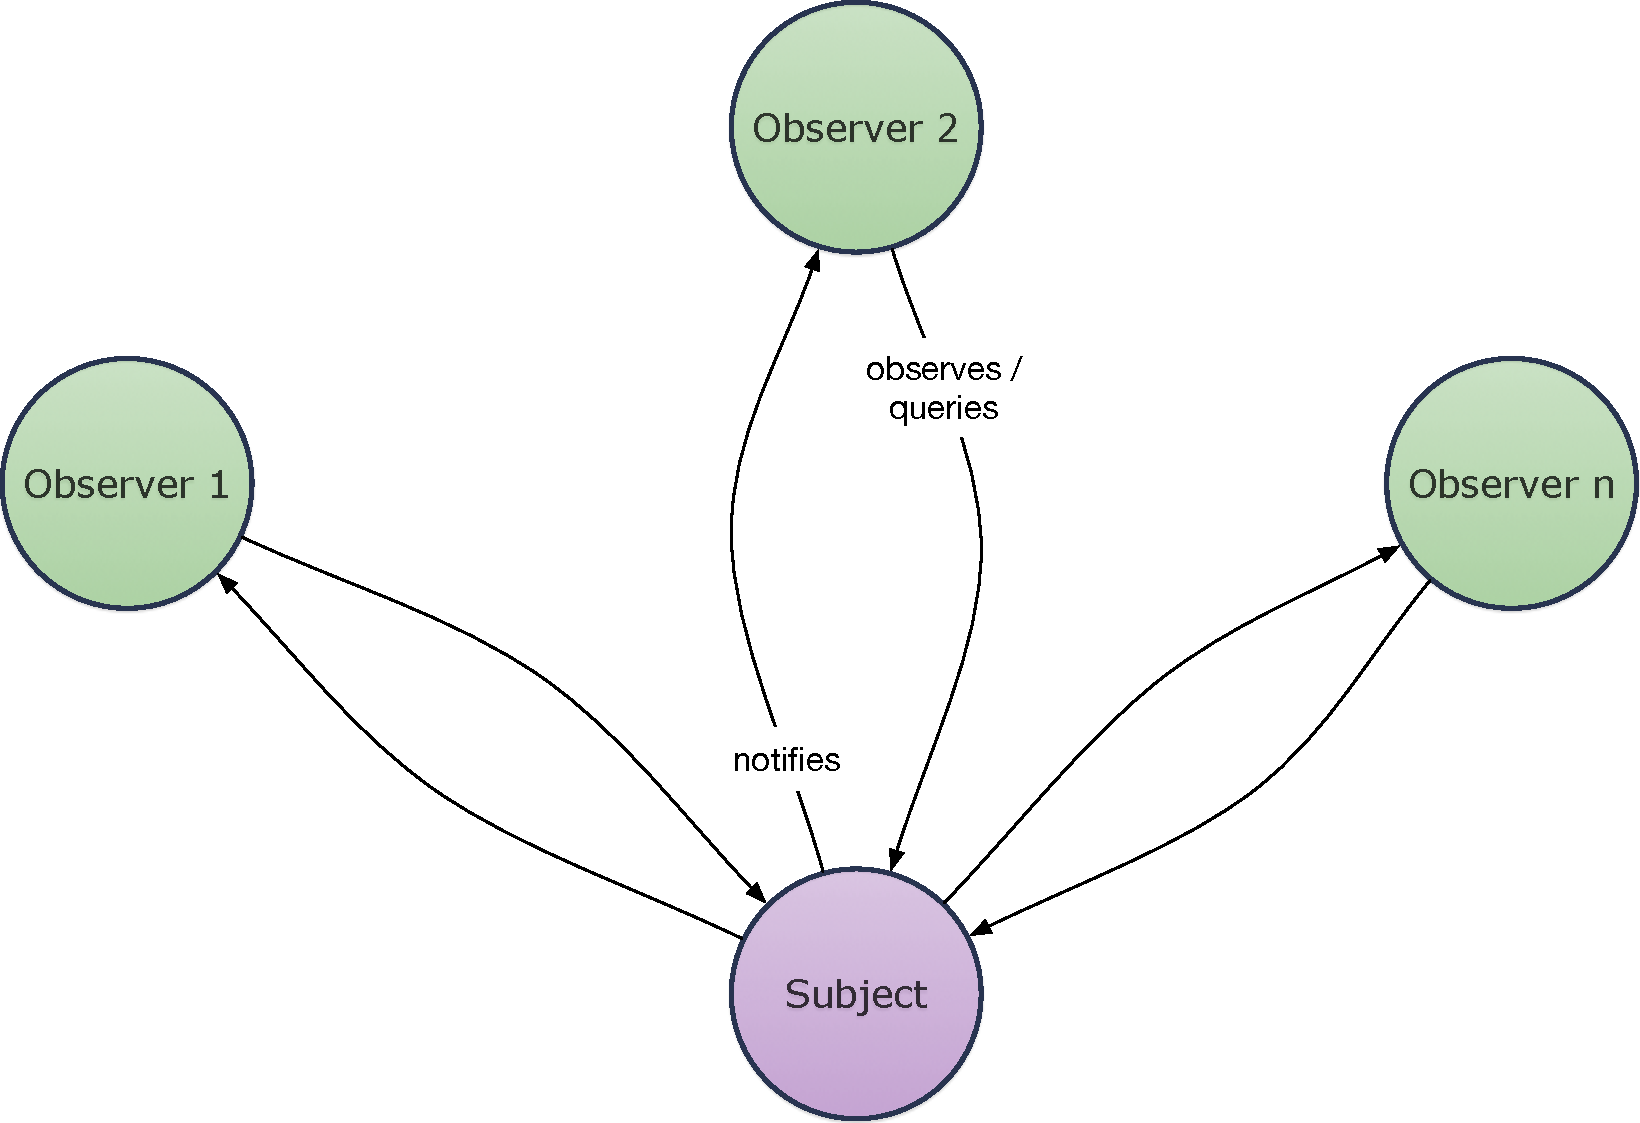
\includegraphics[width=0.8\linewidth]{images/observer-pattern}
  \caption{The observer pattern.~\cite{gamma-dpe-1995}}
  \label{fig:signals-observer-pattern}
\end{figure}

\newthought{A signal is an observable event.} A slot is a potential observer, typically a
function. Slots are registered as observers to signals. Whenever a signal is emitted, the
emitting class must call all the registered observers for that signal. Signals
an slots have a many-to-many relationship. One signal may be connected to any
number of slots and a slot may listen to any number of signals.

\begin{figure}
  \begin{pythoncode}
sender     = Sender()
observer_1 = Observer()

sender.emit_some_signal.connect(
    observer_1.some_slot
)
  \end{pythoncode}
  \label{lst:signal-slot}
  \caption{%
    An example of an observer being registered to a signal.
  }
\end{figure}

\newthought{Signals can hold additional information}, such as single values or
even references to objects. A simple example is loading nodes from files
containing node definitions. The node controller, which loads node definitions
from the file system, could emit two signals to inform other components, for
example components of the GUI layer.
\begin{enumerate*}
  \item The total amount of node definitions to load and
  \item the index of the last loaded node definition including a reference to
    the node definition
\end{enumerate*}
This information could for example be used by a dialog showing the progress of
loading node definitions from the file system. 

\begin{figure}
  \begin{pythoncode}
self.total_node_definitions.emit(num_node_definitions)
  \end{pythoncode}
  \label{lst:signal-slot-example-1}
  \caption{%
    An example of emitting a signal including a value.
  }
\end{figure}

\begin{figure*}
  \begin{pythoncode}
for index, definition_file in enumerate(node_definition_files):
    node_definition = self.load_node_definition_from_file(
        definition_file
    )
    self.node_definition_loaded(index, node_definition)
  \end{pythoncode}
  \label{lst:signal-slot-example-2}
  \caption{%
    An example of emitting a signal including a value and a reference to an
    object.
  }
\end{figure*}

\section{Literate programming}
\label{results:sec:literate-programming}

\newthought{Documentation is crucial to any software project.} However, all too
frequently the documentation is not done properly or is even neglected as it can
be quite effortful with seemingly little benefit. No documentation at all,
outdated or irrelevant documentation can cause unforeseen cost- and time-wise
efforts. Using the literate programming paradigm prevents these problems, as the
software emanates from the documentation. For this thesis literate programming
was used as described in~\ref{sec:literate-programming}.

\todo[inline]{Mention usage of nuweb here, again?}

\newthought{Another train of thought} is required when using literate
programming to develop software than when using traditional methodologies. This
is due to the fact, that the approach is completely different. Traditional
methodologies focus on instructing the computer what to do by writing program
code. Literate programming focuses on explaining to human beings what the
computer shall do by combining the documentation with code fragments in a single
document. From this single document a program which can be compiled or run
directly is extracted. The order of the code fragments matters only indirectly.
They may appear in any order throughout the text. The code fragments are put
into the right order for being compiled or run by defining the output files
containing the needed code fragments in the right order.

\newthought{The need to include every detail} makes literate programming very
expressive and verbose. While this expressiveness may be an advantage for small
software and partly also for larger software, it can also be a problem,
especially for larger software: the documentation can get lengthy and hard to
read, especially when including the implementation of technical details.

\newthought{These aspects} were overcome by moving the implementation into the
appendix~\todo{Insert reference to appendix here.} and by outsourcing similar
and very technical parts and output file definitions into a separate
file.~\todo{Insert reference to code fragments here.}

\section{Software}
\label{results:sec:software}

\newthought{Using the introduced methodologies}
(see~\ref{chap:methodologies}) and the developed software architecture
(see~\ref{results:sec:software-architecture}) the intended software was
developed.
% * Software
% ** Editor
% ** Player
% ** Components% -*- mode: latex; coding: utf-8 -*-

\chapter{Discussion and conclusion}
\label{chap:discussion-conclusion}

\todo[inline]{Write chapter.}

% Im Kapitel Diskussion setzt sich die Autorin, der Autor mit den erzielten
% Ergebnissen auseinander. Diese werden interpretiert und mit Erkenntnissen aus
% anderen Studien zur gleichen Fragestellung beurteilt. Die Diskussion schafft die
% nötigen Grundlagen, damit die in der Einleitung formulierte Fragestellung
% möglichst gut und sachlich richtig beantwortet werden kann.

% In den Folgerungen können die wichtigsten Ergebnisse in ihrer kritischen
% Würdigung prägnant zusammengefasst werden. Es wird eine Art Schlussbilanz
% gezogen. Aus der detaillierten Darstellung der Ergebnisse und deren Diskussion
% lässt sich in der Regel eine Antwort auf die Ausgangsfrage ableiten [3, p. 26].
% Die Antwort auf die Fragestellung kann zu Empfeh- lungen für die Ausführung in
% der Praxis oder für weitere Studien führen. Die Folgerungen dürfen keine neuen
% Elemente und Aspekte enthalten, welche nicht schon in den Ergebnissen und in der
% Diskussion behandelt wurden. Wenn die Problemstellung der Arbeit nur sehr wenige
% Folgerungen verlangt, können diese auch als Schlussteil in die Diskussion
% integriert werden.

% TODO: Check if still needed
% i inc/procedure.w
% i inc/implementation.w


% Backmatter
%---------------------------------------------------------------------------
\backmatter{}

% Appendix
% -*- mode: latex; coding: utf-8 -*-

% \chapter{Appendix}
% \label{chap:appendix}
\appendix
\part*{Appendix}

% -*- mode: latex; coding: utf-8 -*-

\chapter{Implementation}
\label{appendix:chap:implementation}

\newthought{To begin with the implementation} of a project, it is necessary to
first think about the goal that one wants to reach and about some basic
structures and guidelines which lead to the fulfillment of that goal.

\newthought{The main goal is} to have a visual animation system, which allows
the creation and rendering of visually appealing scenes, using a graphical user
interface for creation, and a ray tracing based algorithm for
rendering.~\todo{Adapt goal to current state.}

\newthought{The thoughts to reach this goal} were already developed
in~\nameref{chap:fundamentals} and~\nameref{chap:methodologies} and will
therefore not be repeated again.

\newthought{As stated in~\nameref{chap:methodologies}}, the literate programming
paradigm is used to implement the components. To maintain readability only
relevant code fragments are shown in place. The whole code fragments, which are
needed for tangling, are found at~\nameref{chap:code-fragments}.

\newthought{The editor component is described first} as it is the basis for the
whole project and also contains many concepts, that are re-used by the player
component. Before starting with the implementation it is necessary to define
requirements and some kind of framework for the implementation.

% -*- mode: latex; coding: utf-8 -*-

\section{Requirements}
\label{appendix:sec:requirements}

\newthought{The requirements for running the implementation} are currently the
following:

\begin{itemize}
  \item A Unix derivative as operating system (Linux, macOS).
  \item Python~\footnote{\url{http://www.python.org}} version 3.5.x or above
  \item PyQt5~\footnote{%
      \url{https://riverbankcomputing.com/software/pyqt/intro}} version 5.7 or
    above
  \item OpenGL~\footnote{\url{https://www.opengl.org/}} version 3.3 or above
\end{itemize}% -*- mode: latex; coding: utf-8 -*-

\section{Name spaces and project structure}
\label{appendix:sec:name-spaces}

\newthought{To provide a structure for the whole project} and for being able to
stick to the thoughts established in~\nameref{chap:fundamentals}
and~\nameref{chap:methodologies}, it may be wise to structure the project a
certain way.

\newthought{The source code shall be placed} in the~\verb+src+ directory
underneath the main directory. The creation of the single directories is not
explicitly shown, it is done by parts of this documentation which are tangled
but not exported.

\newthought{When dealing with directories and files}, Python uses the
term~\emph{package} for (sub-) directories and~\emph{module} for files within
directories.\footnote{https://docs.python.org/3/reference/import.html\#packages}

\newthought{To prevent having multiple modules having the same name,} name
spaces are
used.\footnote{https://docs.python.org/3/tutorial/classes.html\#python-scopes-and-namespaces}
The main name space shall be analogous to the project's name:~\verb+qde+.
Underneath the source code folder~\verb+src+, each sub-folder represents a
package and acts therefore also as a name space.

\newthought{To allow a whole package and its modules} being
imported~\emph{as modules}, it needs to have at least a file inside,
called~\verb+__init__.py+. Those files may be empty or they may contain
regular source code such as classes or methods.

\section{Coding style}
\label{appendix:sec:coding-style}

\newthought{To stay consistent throughout implementation} of components, a
coding style is applied which is defined as follows.

\begin{itemize}
  \item Classes use camel case, e.g. \verb+class SomeClassName+.
  \item Folders respectively name spaces use only small letters, e.g.
    \verb+foo.bar.baz+.
  \item Methods are all small caps and use underscores as spaces, e.g.
    \verb+some_method_name+.
  \item Signals are methods, which are prefixed by the word~\enquote{do}, e.g.
    \verb+do_something+.
  \item Slots are methods, which are prefixed by the word~\enquote{on}, e.g.
    \verb+on_something+.
  \item Importing is done by the \verb+from Foo import Bar+ syntax, whereas
    \verb+Foo+ is a module and \verb+Bar+ is either a module, a class or a
    method.
\end{itemize}

\subsection{Importing of modules}
\label{appendix:subsec:imports}

\newthought{For the implementation python is used}, as mentioned
in section~\enquote{\nameref{appendix:sec:requirements}}.
Python has~\enquote{batteries included}, which means that it offers a lot of
functionality through various modules, which have to be imported first before
using them. The same applies of course for self written modules. Python offers
multiple possibilities concerning imports, for details
see~\url{https://docs.python.org/3/tutorial/modules.html}. \todo[inline]{Is
direct url reference ok or does this need to be citation?}

However, PEP number 8 recommends to either import modules directly or to import
the needed functionality
directly.~\footnote{\url{https://www.python.org/dev/peps/pep-0020/}}. As defined
by the coding style,~\autoref{subsec:appendix-implementation-coding-style},
imports are done by the \verb+from Foo import Bar+ syntax.

\newthought{The imported modules are always split up:} first the system modules
are imported, modules which are provided by Python itself or by external
libraries, then project-related modules are imported.

\subsection{Framework for implementation}
\label{appendix:subsec:framework}

\newthought{To stay consistent when implementing} classes an methods, it makes
sense to define a rough framework for their implementation, which is as follows:
\begin{enumerate*}
  \item Define necessary signals,
  \item define the constructor and
  \item implement the remaining functionality in terms of methods and slots.
\end{enumerate*}
Concerning the constructor, the following pattern may be applied:
\begin{enumerate*}
  \item Set up the user interface when it is a class concerning the graphical
    user interface,
  \item set up class-specific aspects, such as the name, the tile or an icon,
  \item set up other components used by that class and
  \item initialize the connections, meaning hooking up the defined signals
    with corresponding methods.
\end{enumerate*}

Now, having defined the~\emph{requirements}, a~\emph{project structure},
a~\emph{coding style} and a~\emph{framework for} the
actual~\emph{implementation}, the implementation of the editor may be
approached.
%-*- mode: latex; coding: utf-8 -*-

\chapter{Editor}
\label{appendix:chap:editor}

\newthought{Before diving right into the implementation} of the editor, it may
be good to reconsider what shall actually be implemented, therefore what the
main functionality of the editor is and what its components are.

\newthought{The quintessence of the editor} is to output a structure, be it in
the JSON format or even in bytecode, which defines an animation.

\newthought{An animation} is simply a composition of scenes which run in a
sequential order within a time span. A scene is then a composition of nodes,
which are at the end of their evaluation nothing else as shader specific code
which gets executed on the GPU. As this definition is rather abstract, it may be
easier to define what shall be achieved in terms of content and then work
towards this definition.

\newthought{A very basic definition of what shall be achieved} is the following.
It shall be possible to create an animated scene using the editor application.
The scene shall be composed of two objects, a sphere and a cube. Additionally it
shall have a camera as well as a point light.

The camera shall be placed 5 units in height and 10 units in front of the center
of the scene. The cube shall be placed in the middle of the scene, the sphere
shall have an offset of 5 units to the right and 2 units in depth. The point
light shall be placed 10 units above the center.

Both objects shall have different materials: the cube shall have a dull surface
of any color whereas the sphere shall have a glossy surface of any color.

There shall be an animation of ten seconds duration. During this animation the
sphere shall move towards the cube and they shall merge into a blob-like object.
The camera shall move 5 units towards the two objects during this time.

\todo[inline]{Scene: Composition of nodes. Define scene already here.}

\newthought{To achieve this overall goal}, while providing an user-friendly
experience, several components are needed. These are the following, being
defined in~\citetitle[pp. 29
ff.]{osterwalder-qde-2016}~\cite{osterwalder-qde-2016}

\begin{description}
  \item[A scene graph] allowing the creation and deletion of scenes. The scene
    graph has at least a root scene.
  \item[A node-based graph] structure allowing the composition of scenes using
    nodes and connections between the nodes. There exists at least a root node
    at the root scene of the scene graph.
  \item[A parameter window] showing parameters of the currently selected graph
    node.
  \item[A rendering window] rendering the currently selected node or scene.
  \item[A sequencer] allowing a time-based scheduling of defined scenes.
\end{description}

However, the above list is not complete. It is somehow intuitively clear, that
there needs to be some~\emph{main component}, which holds all the mentioned
components and allows a proper handling of the application (like managing
resources, shutting down properly and so on).

\newthought{The main component} is composed of a view and a controller, as the
whole architecture uses layers and the MVVMC principle, see
section~\enquote{\nameref{soarch}}. A model is (at least at this point) not
necessary. The view component shall be called~\emph{main window} and its
controller shall be called~\emph{main application}.

\newthought{To preserve clarity} all components described in discrete chapters.
Although the implementation of the components is very specific, in terms of the
programming language, their logic may be reused later on when developing the
player component.

\newthought{Before implementing} any of these components however, the editor
application needs an entry point, that is a point where the application starts
when being called.

\section{Main entry point}
\label{appendix:sec:editor:main}

\newthought{An entry point} is a point where an application starts when being
called. Python does this by evaluating a special variable within a module,
called~\verb+__name__+. Its value is set to \verb+'__main__'+ if the module
is~\enquote{read from standard input, a script, or from an interactive
prompt.}~\footnote{\url{https://docs.python.org/3/library/__main__.html}}

\newthought{All that the entry point needs to do}, in case of the editor
application, is spawning the editor application, execute it and exit again, as
can be seen below.

\begin{figure}[h]
  \begin{flushleft} \small
\begin{minipage}{\linewidth}\label{scrap11}\raggedright\small
\NWtarget{nuweb?}{} $\langle\,${\itshape Main entry point}\nobreak\ {\footnotesize {?}}$\,\rangle\equiv$
\vspace{-1ex}
\begin{pythoncode}
if __name__ == "__main__":
    app = application.Application(sys.argv)
    status = app.exec()
    sys.exit(status)
  |\NWsep|
\end{pythoncode}
\vspace{1.5ex}
\footnotesize
\begin{list}{}{\setlength{\itemsep}{-\parsep}\setlength{\itemindent}{-\leftmargin}}
\item {\NWtxtMacroNoRef}.

\item{}
\end{list}
\end{minipage}\vspace{4ex}
\end{flushleft}
\caption{Main entry point of the editor application.\newline{}\newline{}Editor
    $\rightarrow$ Main entry point}
  \label{editor:lst:main}
\end{figure}

\newthought{But where to place the main entry point?} A very direct approach
would be to implement that main entry point within the main application
controller. But when running the editor application by calling it from the
command line, calling a controller directly may rather be confusing. Instead it
is more intuitive to have only a minimal entry point which is clearly visible as
such. Therefore the main entry point will be put in a file
called~\verb+editor.py+ which is at the top level of the~\verb+src+ directory.

\section{Main application}
\label{appendix:sec:editor:app}

\newthought{The editor application cannot be started yet}, although a main entry
point is defined by now. This is due the fact that there is no such thing as an
editor application yet. Therefore a main application needs to implemented.

\newthought{Qt version 5 is used} through the PyQt5 wrapper, as stated in the
section~\enquote{\nameref{appendix:sec:requirements}}. Therefore all
functionality of Qt 5 may be used. Qt already offers a main application class,
which can be used as a controller. The class is called~\verb+QApplication+.

\newthought{But what does such a main application class actually do?} What is
its functionality? Very roughly sketched, such a type of application initializes
resources, enters a main loop, where it stays until told to shut down, and at
the end it frees the allocated resources again.

Due to the usage of~\verb+QApplication+ as super class it is not necessary to
implement a main (event-) loop, as such is provided by Qt
itself~\footnote{http://doc.qt.io/Qt-5/qapplication.html\#exec}.

As the main application initializes resources, it act as central node between the
various layers of the architecture, initializing them and connecting them using
signals.\cite[pp. 37 --- 38]{osterwalder-qde-2016}

\begin{figure}[h]
  \begin{flushleft} \small
\begin{minipage}{\linewidth}\label{scrap12}\raggedright\small
\NWtarget{nuweb?}{} $\langle\,${\itshape Main application declarations}\nobreak\ {\footnotesize {?}}$\,\rangle\equiv$
\vspace{-1ex}
\begin{pythoncode}
  |\normalfont{}\fontfamily{}|common.with_logger
  class Application(QtWidgets.QApplication):
      """Main application for QDE."""

      |\hbox{$\langle\,${\itshape Main application constructor}\nobreak\ {\footnotesize \NWlink{nuweb?}{?}}$\,\rangle$}|
      |\hbox{$\langle\,${\itshape Main application methods}\nobreak\ {\footnotesize ?}$\,\rangle$}||\NWsep|
\end{pythoncode}
\vspace{1.5ex}
\footnotesize
\begin{list}{}{\setlength{\itemsep}{-\parsep}\setlength{\itemindent}{-\leftmargin}}
\item {\NWtxtMacroNoRef}.

\item{}
\end{list}
\end{minipage}\vspace{4ex}
\end{flushleft}
\caption{Main application class of the editor
    application.\newline{}\newline{}Editor $\rightarrow$ Application}
  \label{editor:lst:app}
\end{figure}

Therefore it needs to do at least three things:
\begin{enumerate*}
  \item initialize itself,
  \item set up components and
  \item connect components.
  \end{enumerate*}
This all happens when the main application is being initialized through its
constructor.

\begin{figure}[h]
\begin{flushleft} \small
\begin{minipage}{\linewidth}\label{scrap13}\raggedright\small
\NWtarget{nuweb?}{} $\langle\,${\itshape Main application constructor}\nobreak\ {\footnotesize {?}}$\,\rangle\equiv$
\vspace{-1ex}
\begin{pythoncode}
def __init__(self, arguments):
    """Constructor.

    :param arguments: a (variable) list of arguments, that are
                      passed when calling this class.
    :type  argv:      list
    """

    |\hbox{$\langle\,${\itshape Set up internals for main application}\nobreak\ {\footnotesize \NWlink{nuweb?}{?}}$\,\rangle$}|
    |\hbox{$\langle\,${\itshape Set up components for main application}\nobreak\ {\footnotesize \NWlink{nuweb?}{?}}$\,\rangle$}|
    |\hbox{$\langle\,${\itshape Add root node for main application}\nobreak\ {\footnotesize ?}$\,\rangle$}|
    |\hbox{$\langle\,${\itshape Set model for scene graph view}\nobreak\ {\footnotesize ?}$\,\rangle$}|
    |\hbox{$\langle\,${\itshape Load nodes}\nobreak\ {\footnotesize ?}$\,\rangle$}|
    self.main_window.show()|\NWsep|
\end{pythoncode}
\vspace{1.5ex}
\footnotesize
\begin{list}{}{\setlength{\itemsep}{-\parsep}\setlength{\itemindent}{-\leftmargin}}
\item \NWtxtMacroRefIn\ \NWlink{nuweb?}{?}.

\item{}
\end{list}
\end{minipage}\vspace{4ex}
\end{flushleft}
\caption{Constructor of the editor application
    class.\newline{}\newline{}Editor $\rightarrow$ Application $\rightarrow$
    Constructor} \label{editor:lst:app:constructor}
\end{figure}

\newthought{Setting up the internals} is straight forward: Passing any given
arguments directly to~\verb+QApplication+, setting an application icon, a name
as well as a display name.

\begin{figure}[h]
\begin{flushleft} \small
\begin{minipage}{\linewidth}\label{scrap14}\raggedright\small
\NWtarget{nuweb?}{} $\langle\,${\itshape Set up internals for main application}\nobreak\ {\footnotesize {?}}$\,\rangle\equiv$
\vspace{-1ex}
\begin{pythoncode}
super(Application, self).__init__(arguments)
self.setWindowIcon(QtGui.QIcon("assets/icons/im.png"))
self.setApplicationName("QDE")
self.setApplicationDisplayName("QDE")|\NWsep|
\end{pythoncode}
\vspace{1.5ex}
\footnotesize
\begin{list}{}{\setlength{\itemsep}{-\parsep}\setlength{\itemindent}{-\leftmargin}}
\item \NWtxtMacroRefIn\ \NWlink{nuweb?}{?}.

\item{}
\end{list}
\end{minipage}\vspace{4ex}
\end{flushleft}
\caption{Setting up the internals for the main application class.
  \newline{}\newline{}Editor $\rightarrow$ Application $\rightarrow$
  Constructor} \label{editor:lst:app:constructor:internals}
\end{figure}

The other two steps, setting up the components and connecting them can however
not be done at this point, as there simply are no components available. A
component to start with is the view component of the main application, the main
window.

\section{Main window}
\label{appendix:sec:editor:main-window}

\newthought{Having a very basic implementation} of the main application, its
view component, the main window, can now be implemented and then be set up by
the main application.

\newthought{The main functionality} of the main window is to set up the actual
user interface, containing all the views of the components. Qt offers the class
\verb+QMainWindow+ from which \verb=MainWindow= may inherit.

\begin{figure}
\begin{flushleft} \small
\begin{minipage}{\linewidth}\label{scrap15}\raggedright\small
\NWtarget{nuweb?}{} $\langle\,${\itshape Main window declarations}\nobreak\ {\footnotesize {?}}$\,\rangle\equiv$
\vspace{-1ex}
\begin{pythoncode}
|\normalfont{}\fontfamily{}|common.with_logger
class MainWindow(QtWidgets.QMainWindow):
    """The main window class.
    Acts as main view for the QDE editor application.
    """

    |\hbox{$\langle\,${\itshape Main window signals}\nobreak\ {\footnotesize \NWlink{nuweb?}{?}}$\,\rangle$}|

    |\hbox{$\langle\,${\itshape Main window methods}\nobreak\ {\footnotesize \NWlink{nuweb?}{?}, \ldots\ }$\,\rangle$}|
|\NWsep|
\end{pythoncode}
\vspace{1.5ex}
\footnotesize
\begin{list}{}{\setlength{\itemsep}{-\parsep}\setlength{\itemindent}{-\leftmargin}}
\item {\NWtxtMacroNoRef}.

\item{}
\end{list}
\end{minipage}\vspace{4ex}
\end{flushleft}
\caption{Main window class of the editor application.
  \newline{}\newline{}Editor $\rightarrow$ Main window}
  \label{editor:lst:main-window}
\end{figure}
% AT<Main window slotsAT>

\newthought{For being able to shut down} the main application and therefore the
main window, they need to react to a request for shutting down, either by a
keyboard shortcut or a menu command. However, the main window is not able to
force the main application to quit by itself. It would be possible to pass the
main window a reference to the application, but that would lead to tight
coupling and is therefore not considered as an option. Signals and slots allow
exactly such cross-layer communication without coupling components tightly.

\newthought{To avoid tight coupling} a signal within the main window is
introduced, which tells the main application to shut down. A fitting name for
the signal might be~\verb=do_close=.

\begin{figure}
\begin{flushleft} \small
\begin{minipage}{\linewidth}\label{scrap16}\raggedright\small
\NWtarget{nuweb?}{} $\langle\,${\itshape Main window signals}\nobreak\ {\footnotesize {?}}$\,\rangle\equiv$
\vspace{-1ex}
\begin{pythoncode}
do_close = QtCore.pyqtSignal()|\NWsep|
\end{pythoncode}
\vspace{1.5ex}
\footnotesize
\begin{list}{}{\setlength{\itemsep}{-\parsep}\setlength{\itemindent}{-\leftmargin}}
\item \NWtxtMacroRefIn\ \NWlink{nuweb?}{?}.

\item{}
\end{list}
\end{minipage}\vspace{4ex}
\end{flushleft}
\caption{Definition of the~\texttt{do\_close} signal of the main window class.
  \newline{}\newline{}Editor $\rightarrow$ Main window $\rightarrow$ Signals}
\label{editor:lst:main-window:signals}
\end{figure}

Now, that the signal for closing the window and the application is defined, two
additional things need to be considered: The emission of the signal by
the main window itself as well as the consumption of the signal by a slot of
other classes.

The signal shall be emitted when the escape key on the keyboard is pressed or
when the corresponding menu item was selected. As there is no menu at the
moment, only the key pressed event is implemented by now.

\begin{figure}
\begin{flushleft} \small
\begin{minipage}{\linewidth}\label{scrap17}\raggedright\small
\NWtarget{nuweb?}{} $\langle\,${\itshape Main window methods}\nobreak\ {\footnotesize {?}}$\,\rangle\equiv$
\vspace{-1ex}
\begin{pythoncode}
def __init__(self, parent=None):
    """Constructor."""

    super(MainWindow, self).__init__(parent)
    self.setup_ui()

def keyPressEvent(self, event):
    """Gets triggered when a key press event is raised.

    :param event: holds the triggered event.
    :type  event: QKeyEvent
    """

    if event.key() == QtCore.Qt.Key_Escape:
        self.do_close.emit()
    else:
        super(MainWindow, self).keyPressEvent(event)
|\NWsep|
\end{pythoncode}
\vspace{1.5ex}
\footnotesize
\begin{list}{}{\setlength{\itemsep}{-\parsep}\setlength{\itemindent}{-\leftmargin}}
\item \NWtxtMacroDefBy\ \NWlink{nuweb?}{?}\NWlink{nuweb?}{, ?}.
\item \NWtxtMacroRefIn\ \NWlink{nuweb?}{?}.

\item{}
\end{list}
\end{minipage}\vspace{4ex}
\end{flushleft}
\caption{Definition of methods for the main window class.
  \newline{}\newline{}Editor $\rightarrow$ Main window $\rightarrow$ Methods}
\label{editor:lst:main-window:methods}
\end{figure}

% For emitting the signal when selecting a menu entry, an action needs to be
% defined which is then attached to the menu entry. The action emits a signal as
% soon as the menu entry was clicked. It is however not possible to trigger the
% defined \verb+do_close+ signal using the actions signal. There a slot needs to
% be defined which then in its turn triggers \verb+do_close+.

\newthought{The main window can now be set up} by the main application
controller, which also listens to the~\verb=do_close= signal through the
inherited~\verb=quit= slot.

\begin{figure}
\begin{flushleft} \small
\begin{minipage}{\linewidth}\label{scrap18}\raggedright\small
\NWtarget{nuweb?}{} $\langle\,${\itshape Set up components for main application}\nobreak\ {\footnotesize {?}}$\,\rangle\equiv$
\vspace{-1ex}
\begin{pythoncode}
|\hbox{$\langle\,${\itshape Set up controllers for main application}\nobreak\ {\footnotesize ?}$\,\rangle$}|
|\hbox{$\langle\,${\itshape Connect controllers for main application}\nobreak\ {\footnotesize ?}$\,\rangle$}|
|\hbox{$\langle\,${\itshape Set up main window for main application}\nobreak\ {\footnotesize \NWlink{nuweb?}{?}}$\,\rangle$}||\NWsep|
\end{pythoncode}
\vspace{1.5ex}
\footnotesize
\begin{list}{}{\setlength{\itemsep}{-\parsep}\setlength{\itemindent}{-\leftmargin}}
\item \NWtxtMacroRefIn\ \NWlink{nuweb?}{?}.

\item{}
\end{list}
\end{minipage}\vspace{4ex}
\end{flushleft}
\caption{Setting up of components for the main application class.
  \newline{}\newline{}Editor $\rightarrow$ Main application $\rightarrow$
  Constructor}
\label{editor:lst:main-application:constructor:methods}
\end{figure}

\begin{figure}
\begin{flushleft} \small
\begin{minipage}{\linewidth}\label{scrap19}\raggedright\small
\NWtarget{nuweb?}{} $\langle\,${\itshape Set up main window for main application}\nobreak\ {\footnotesize {?}}$\,\rangle\equiv$
\vspace{-1ex}
\begin{pythoncode}
self.main_window = qde_main_window.MainWindow()
self.main_window.do_close.connect(self.quit)
|\hbox{$\langle\,${\itshape Connect main window components}\nobreak\ {\footnotesize ?}$\,\rangle$}||\NWsep|
\end{pythoncode}
\vspace{1.5ex}
\footnotesize
\begin{list}{}{\setlength{\itemsep}{-\parsep}\setlength{\itemindent}{-\leftmargin}}
\item \NWtxtMacroRefIn\ \NWlink{nuweb?}{?}.

\item{}
\end{list}
\end{minipage}\vspace{4ex}
\end{flushleft}
\caption{Set up of the editor main window and its signals from within the main
  application. \newline{}\newline{}Editor $\rightarrow$ Main application
  $\rightarrow$ Constructor}
\label{editor:lst:main-application:constructor:main-window}
\end{figure}

The used view component for the main window,~\verb+QMainWindow+, needs at least
a central widget with a layout for being
rendered.~\footnote{http://doc.qt.io/qt-5/qmainwindow.html\#creating-main-window-components}

\newthought{As the main window will set up and hold} the whole layout for the
application through multiple view components, a method~\verb+setup_ui+ is
introduced, which sets up the whole layout. The method creates a central widget
containing a grid layout.

\newthought{Targeting a look} as proposed in~\citetitle[p.
9]{osterwalder-qde-2016}, a simple grid layout does however not provide enough
possibilities. Instead a horizontal box layout in combination with splitters is
used.

Recalling the components, the following layout is approached:

\begin{itemize}
\item{%
    A scene graph, on the left of the window, covering the whole height.}
\item{%
    A node graph on the right of the scene graph, covering as much height as
    possible.}
\item{%
    A view for showing the properties (and therefore parameters) of the selected
    node on the right of the node graph, covering as much height as possible.}
\item{%
    A display for rendering the selected node, on the right of the properties
    view, covering as much height as possible}
\item{%
    A sequencer at the right of the scene graph and below the other components
    at the bottom of the window, covering as much width as possible}
\end{itemize}

\todo[inline]{Provide a picture of the layout here.}

\begin{figure*}
\begin{flushleft} \small
\begin{minipage}{\linewidth}\label{scrap20}\raggedright\small
\NWtarget{nuweb?}{} $\langle\,${\itshape Main window methods}\nobreak\ {\footnotesize {?}}$\,\rangle+\equiv$
\vspace{-1ex}
\begin{pythoncode}
def setup_ui(self):
    """Sets up the user interface specific components."""

    self.setObjectName('MainWindow')
    self.setWindowTitle('QDE')
    self.resize(1024, 768)
    self.move(100, 100)
    # Ensure that the window is not hidden behind other windows
    self.activateWindow()

    central_widget = QtWidgets.QWidget(self)
    central_widget.setObjectName('central_widget')
    grid_layout = QtWidgets.QGridLayout(central_widget)
    central_widget.setLayout(grid_layout)
    self.setCentralWidget(central_widget)
    self.statusBar().showMessage('Ready.')

    horizontal_layout_widget = QtWidgets.QWidget(central_widget)
    horizontal_layout_widget.setObjectName('horizontal_layout_widget')
    horizontal_layout_widget.setGeometry(QtCore.QRect(12, 12, 781, 541))
    horizontal_layout_widget.setSizePolicy(QtWidgets.QSizePolicy.MinimumExpanding,
    QtWidgets.QSizePolicy.MinimumExpanding)
    grid_layout.addWidget(horizontal_layout_widget, 0, 0)

    horizontal_layout = QtWidgets.QHBoxLayout(horizontal_layout_widget)
    horizontal_layout.setObjectName('horizontal_layout')
    horizontal_layout.setContentsMargins(0, 0, 0, 0)

    self.scene_graph_view = guiscene.SceneGraphView()
    self.scene_graph_view.setObjectName('scene_graph_view')
    self.scene_graph_view.setMaximumWidth(300)
    horizontal_layout.addWidget(self.scene_graph_view)

    |\hbox{$\langle\,${\itshape Set up scene view in main window}\nobreak\ {\footnotesize ?}$\,\rangle$}|
    |\hbox{$\langle\,${\itshape Set up parameter view in main window}\nobreak\ {\footnotesize ?}$\,\rangle$}|
    |\hbox{$\langle\,${\itshape Set up render view in main window}\nobreak\ {\footnotesize ?}$\,\rangle$}|

    horizontal_splitter = QtWidgets.QSplitter()
    |\hbox{$\langle\,${\itshape Add render view to horizontal splitter in main window}\nobreak\ {\footnotesize ?}$\,\rangle$}|
    |\hbox{$\langle\,${\itshape Add parameter view to horizontal splitter in main window}\nobreak\ {\footnotesize ?}$\,\rangle$}|

    vertical_splitter = QtWidgets.QSplitter()
    vertical_splitter.setOrientation(QtCore.Qt.Vertical)
    vertical_splitter.addWidget(horizontal_splitter)
    |\hbox{$\langle\,${\itshape Add scene view to vertical splitter in main window}\nobreak\ {\footnotesize ?}$\,\rangle$}|

    horizontal_layout.addWidget(vertical_splitter)
|\NWsep|
\end{pythoncode}
\vspace{1.5ex}
\footnotesize
\begin{list}{}{\setlength{\itemsep}{-\parsep}\setlength{\itemindent}{-\leftmargin}}
\item \NWtxtMacroDefBy\ \NWlink{nuweb?}{?}\NWlink{nuweb?}{, ?}.
\item \NWtxtMacroRefIn\ \NWlink{nuweb?}{?}.

\item{}
\end{list}
\end{minipage}\vspace{4ex}
\end{flushleft}
\caption{Set up of the user interface of the editor's  main window.
  \newline{}\newline{}Editor $\rightarrow$ Main window
  $\rightarrow$ Methods}
\label{editor:lst:main-window:methods:setup-ui}
\end{figure*}

All the above taken actions to lay out the main window change nothing in the
window's yet plain appearance. This is quite obvious, as none of the actual
components are implemented yet.

\newthought{A good starting point} for the implementation of the remaining
components might be the scene graph, as it might be the most straight-forward
component to implement.

\chapter{Scene graph}
\label{appendix:chap:scene-graph}

\newthought{The scene graph component} has two aspects to consider, as mentioned
in chapter~\enquote{\nameref{appendix:chap:editor}}:
\begin{enumerate*}
  \item a graphical aspect as well as
  \item its data structure.
\end{enumerate*}

\todo[inline]{Define what a scene is by prose and code.}

As described in subsection~\enquote{\nameref{results:subsec:software-design}},
two kinds of models are used. A domain model, containing the actual data and a
view model, which holds a reference to its corresponding domain model.

% \todo[inline]{Check whether to move into procedure.}
% Both models are managed by the same controller. View models are displayed by views,
% e.g. node view models in the node graph view.
%
% Therefore the controller of the scene graph will manage instances of scene
% domain models whereas the view of the scene graph will display a tree of scene
% view models.

As the domain model builds the basis for the whole (data-) structure, it is
implemented first.

\begin{figure}
\begin{flushleft} \small
\begin{minipage}{\linewidth}\label{scrap21}\raggedright\small
\NWtarget{nuweb?}{} $\langle\,${\itshape Scene model declarations}\nobreak\ {\footnotesize {?}}$\,\rangle\equiv$
\vspace{-1ex}
\begin{pythoncode}
class SceneModel(object):
    """The scene model.
    It is used as a base class for scene instances within the
    whole system.
    """

    |\hbox{$\langle\,${\itshape Scene model signals}\nobreak\ {\footnotesize ?}$\,\rangle$}|
    |\hbox{$\langle\,${\itshape Scene model methods}\nobreak\ {\footnotesize \NWlink{nuweb?}{?}}$\,\rangle$}|
    |\hbox{$\langle\,${\itshape Scene model slots}\nobreak\ {\footnotesize ?}$\,\rangle$}||\NWsep|
\end{pythoncode}
\vspace{1.5ex}
\footnotesize
\begin{list}{}{\setlength{\itemsep}{-\parsep}\setlength{\itemindent}{-\leftmargin}}
\item {\NWtxtMacroNoRef}.

\item{}
\end{list}
\end{minipage}\vspace{4ex}
\end{flushleft}
\caption{Definition of the scene model class, which acts as a base class for
scene instances within the whole application.
  \newline{}\newline{}Editor $\rightarrow$ Scene model}
\label{editor:lst:scene-model}
\end{figure}

\newthought{The only known fact} at this point is, that a scene is a composition
of nodes and therefore holds its nodes as a list. Additionally it holds a
reference to its parent.

\begin{figure}
\begin{flushleft} \small
\begin{minipage}{\linewidth}\label{scrap22}\raggedright\small
\NWtarget{nuweb?}{} $\langle\,${\itshape Scene model methods}\nobreak\ {\footnotesize {?}}$\,\rangle\equiv$
\vspace{-1ex}
\begin{pythoncode}
def __init__(self, parent=None):
    """Constructor.

    :param parent: the parent scene of this scene. The parent is
                   None if the current scene is the root scene.
    :type parent:  SceneModel
    """

    self.id_ = uuid.uuid4()
    self.nodes = []
    self.parent = parent|\NWsep|
\end{pythoncode}
\vspace{1.5ex}
\footnotesize
\begin{list}{}{\setlength{\itemsep}{-\parsep}\setlength{\itemindent}{-\leftmargin}}
\item \NWtxtMacroRefIn\ \NWlink{nuweb?}{?}.

\item{}
\end{list}
\end{minipage}\vspace{4ex}
\end{flushleft}
\caption{The constructor of the scene model.
  \newline{}\newline{}Editor $\rightarrow$ Scene model $\rightarrow$ Constructor}
\label{editor:lst:scene-model:constructor}
\end{figure}

% The counter part of the domain model is the view model. View models are used to
% visually represent something within the graphical user interface and they
% provide an interface to the \verb+domain+ layer. To this point, a simple
% reference in terms of an attribute is used as interface, which may be changed
% later on.
% 
% Concerning the user interface, a view model must fulfill the requirements posed
% by the user interface's corresponding component. In this case, this are actually
% two components: the scene graph view as well as the scene view.
% 
% It would therefore make sense the use one view model for both components, but
% this is not possible as the view model of the scene view, \verb+QGraphicsScene+,
% uses its own data model.
% 
% Therefore \verb+QObject+ will be used for the scene graph view model and
% \verb+QGraphicsScene+ will be used for the scene view model.
% 
% ATd Scene graph view model declarations
% AT{
% class SceneGraphViewModel(Qt.QObject):
%     """View model representing scene graph items.
% 
%     The SceneGraphViewModel corresponds to an entry within the scene graph. It is
%     used by the QAbstractItemModel class and must therefore at least provide a
%     name and a row.
%     """
% 
%     AT<Scene graph view model signalsAT>
% 
%     AT<Scene graph view model constructorAT>
% 
%     AT<Scene graph view model methodsAT>
% 
%     AT<Scene graph view model slotsAT>
% AT}
% 
% In terms of the scene graph, the view model must provide at least a name and a
% row. In addition, as written above, it holds a reference to the domain model.
% 
% ATd Scene graph view model constructor
% AT{
% def __init__(
%         self,
%         row,
%         domain_object,
%         name=QtCore.QCoreApplication.translate('SceneGraphViewModel', 'New scene'),
%         parent=None
% ):
%     """Constructor.
% 
%     :param row:           The row the view model is in.
%     :type  row:           int
%     :param domain_object: Reference to a scene model.
%     :type  domain_object: qde.editor.domain.scene.SceneModel
%     :param name:          The name of the view model, which will be displayed in
%                           the scene graph.
%     :type  name:          str
%     :param parent:        The parent of the current view model within the scene
%                           graph.
%     :type parent:         qde.editor.gui_domain.scene.SceneGraphViewModel
%     """
% 
%     super(SceneGraphViewModel, self).__init__(parent)
% 
%     self.id_ = domain_object.id_
%     self.row  = row
%     self.domain_object = domain_object
%     self.name = name
% AT}
% 
% Scenes may now be instantiated, it is although necessary to manage scenes in a
% controlled manner. Therefore the class \verb+SceneGraphController+ will now be
% implemented, for being able to manage scenes.
% 
% As the scene graph shall be built as a tree structure, an appropriate data
% structure is needed. Qt provides the \verb+QTreeWidget+ class, but that
% class is in this case not suitable, as it does not separate the data from its
% representation, as stated by Qt:~\enquote{Developers who do not need the flexibility of
% the Model/View framework can use this class to create simple hierarchical lists
% very easily. A more flexible approach involves combining a QTreeView with a
% standard item model. This allows the storage of data to be separated from its
% representation.}\footnote{http://doc.qt.io/qt-5/qtreewidget.html\#details}
% 
% Such a standard item model is
% \verb+QAbstractItemModel+\footnote{\label{footnote:qabstractitemmodel}
% http://doc.qt.io/qt-5/qabstractitemmodel.html}, which is used as a base class
% for the scene graph controller.
% 
% ATd Scene graph controller declarations
% AT{
% ATATcommon.with_logger
% class SceneGraphController(QtCore.QAbstractItemModel):
%     """The scene graph controller.
%     A controller for managing the scene graph by adding, editing and removing
%     scenes.
%     """
% 
%     AT<Scene graph controller signalsAT>
% 
%     AT<Scene graph controller constructorAT>
%     AT<Scene graph controller methodsAT>
% 
%     AT<Scene graph controller slotsAT>
% AT}
% 
% As at this point the functionality of the scene graph controller is not fully
% known, the constructor simply initializes its parent class and an empty list of
% scenes.
% 
% ATd Scene graph controller constructor
% AT{
% def __init__(self, parent=None):
%     """Constructor.
% 
%     :param parent: The parent of the current view model within the scene
%                     graph.
%     :type parent:  qde.editor.gui_domain.scene.SceneGraphViewModel
%     """
% 
%     super(SceneGraphController, self).__init__(parent)
% AT}
% 
% As the scene graph controller holds and manages the data, it needs to have at
% least a root node. As the controller manages both, domain models and the view
% models, it needs to create both models.
% 
% Due to the dependencies of other components this cannot be done within the
% constructor, as components dependening on the scene graph controller may not be
% listening to its signals at this point. Therefore this is done in a separate
% method called \verb+add_root_node+.
% 
% ATd Scene graph controller add root node
% AT{
% def add_root_node(self):
%     """Add a root node to the data structure.
%     """
% 
%     if self.root_node is None:
%         root_node = domain_scene.SceneModel()
%         self.view_root_node = guidomain_scene.SceneGraphViewModel(
%             row=0,
%             domain_object=root_node,
%             name=QtCore.QCoreApplication.translate(__class__.__name__, 'Root scene')
%         )
%         self.do_add_scene.emit(root_node)
%         self.layoutChanged.emit()
%         self.logger.debug("Added root node")
%     else:
%         self.logger.warn("Not (re-) adding root node, already present!")
% AT}
% ATd Scene graph controller methods
% AT{
% AT<Scene graph controller add root nodeAT>
% AT}
% 
% % TODO
% The root scene can then be added by the main application, when all components
% are set up properly.
% 
% ATd Add root node for main application
% AT{self.scene_graph_controller.add_root_node()AT}
% 
% The scene graph controller must also provide the header data, which is used to
% display the header within the view (due to the usage of the Qt view
% model\todo{Add reference to Qts view model}). As header data the name of the
% scenes as well as the number of nodes a scene contains shall be displayed.
% 
% ATd Scene graph controller constructor
% AT{
%     self.header_data = [
%         QtCore.QCoreApplication.translate(__class__.__name__, 'Name'),
%         QtCore.QCoreApplication.translate(__class__.__name__, '# Nodes')
%     ]
%     self.root_node = None
%     self.view_root_node = None
% AT}
% 
% % TODO: Check if needed
% % Before implementing the actual methods, it is important to think about the
% % attributes, that the scene graph controller will have, as attributes define and
% % influence the methods.
% 
% As \verb+QAbstractItemModel+ is used as a basis for the scene graph controller,
% some methods must be implemented at very least:~\enquote{When subclassing
% QAbstractItemModel, at the very least you must implement index(), parent(),
% rowCount(), columnCount(), and data(). These functions are used in all read-only
% models, and form the basis of editable
% models.}\footref{footnote:qabstractitemmodel}
% 
% The method \verb+index+ returns the position of an item in the (data-) model for
% a given row and column below a parent item.
% 
% ATd Scene graph controller methods
% AT{
% def index(self, row, column, parent=QtCore.QModelIndex()):
%     """Return the index of the item in the model specified by the given row,
%     column and parent index.
% 
%     :param row: The row for which the index shall be returned.
%     :type  row: int
%     :param column: The column for which the index shall be returned.
%     :type column: int
%     :param parent: The parent index of the item in the model. An invalid model
%                    index is given as the default parameter.
%     :type parent: QtQore.QModelIndex
% 
%     :return: the model index based on the given row, column and the parent
%              index.
%     :rtype: QtCore.QModelIndex
%     """
% 
%     if not parent.isValid():
%         self.logger.debug((
%             "Getting index for row {0}, col {1}, root node"
%         ).format(row, column))
%         return self.createIndex(row, column, self.view_root_node)
% 
%     parent_node = parent.internalPointer()
%     self.logger.debug((
%         "Getting index for row {0}, col {1}, parent {2}. Children: {3}"
%     ).format(row, column, parent_node, len(parent_node.children())))
%     child_nodes = parent_node.children()
% 
%     # It may happen, that the index is called at the same time as a node is
%     # being deleted respectively was deleted. In this case an invalid index is
%     # returned.
%     try:
%         child_node  = child_nodes[row]
%         return self.createIndex(row, column, child_node)
% 
%     except IndexError:
%         return QtCore.QModelIndex()AT}
% 
% The method \verb+parent+ returns the parent item of an item identified by a
% provided index. If that index is invalid, an invalid index is returned as well.
% 
% ATd Scene graph controller methods
% AT{
% def parent(self, model_index):
%     """Return the parent of the model item with the given index. If the item has
%     no parent, an invalid QModelIndex is returned.
% 
%     :param model_index: The model index which the parent model index shall be
%                         derived for.
%     :type model_index: int
% 
%     :return: the model index of the parent model item for the given model index.
%     :rtype: QtCore.QModelIndex
%     """
% 
%     # self.logger.debug("Getting parent")
% 
%     if not model_index.isValid():
%         # self.logger.debug("No valid index for parent")
%         return QtCore.QModelIndex()
% 
%     # The internal pointer of the the model index returns a scene graph view
%     # model.
%     node = model_index.internalPointer()
%     if node and node.parent() is not None:
%         # self.logger.debug("Index for parent")
%         return self.createIndex(node.parent().row, 0, node.parent())
%     else:
%         # self.logger.debug("Index for root")
%         return QtCore.QModelIndex()
% AT}
% 
% Implementing the \verb+columnCount+ and \verb+rowCount+ methods is straight
% forward. The former returns simply the number of columns, in this case the
% number of headers, therefore 2.
% 
% ATd Scene graph controller methods
% AT{
% def columnCount(self, parent):
%     """Return the number of columns for the children of the given parent.
% 
%     :param parent: The index of the item in the scene graph, which the
%                     column count shall be returned for.
%     :type  parent: QtCore.QModelIndex
% 
%     :return: the number of columns for the children of the given parent.
%     :rtype:  int
%     """
% 
%     column_count = len(self.header_data) - 1
%     self.logger.debug("Getting column count: %s", column_count)
% 
%     return column_count
% AT}
% 
% The method \verb+rowCount+ returns the number of nodes for a given parent
% item (identified by its index within the data model).
% 
% ATd Scene graph controller methods
% AT{
% def rowCount(self, parent):
%     """Return the number of rows for the children of the given parent.
% 
%     :param parent: The index of the item in the scene graph, which the
%                     row count shall be returned for.
%     :type  parent: QtCore.QModelIndex
% 
%     :return: the number of rows for the children of the given parent.
%     :rtype:  int
%     """
% 
%     if not parent.isValid():
%         self.logger.debug("Parent is not valid")
%         row_count = 1
%     else:
%         # Get the actual object stored by the parent. In this case it is a
%         # SceneGraphViewModel.
%         node = parent.internalPointer()
% 
%         if node is None:
%             self.logger.debug("Parent (node) is not valid")
%             row_count = 1
%         else:
%             row_count = len(node.children())
% 
%     self.logger.debug("Getting row count: %s", row_count)
%     return row_count
% AT}
% 
% The last method, that has to be implemented due to the usage of
% \verb+QAbstractItemModel+, is the \verb+data+ method. It returns the data for an
% item identified by the given index for the given role.
% 
% A role indicates what type of data is provided. Currently the only role
% considered is the display of models (further information may be found
% at~\url{http://doc.qt.io/qt-5/qt.html#ItemDataRole-enum}).
% 
% Depending on the column of the model index, the method returns either the name
% of the scene graph node or the number of nodes a scene contains.
% 
% ATd Scene graph controller methods
% AT{
% def data(self, model_index, role=QtCore.Qt.DisplayRole):
%     """Return the data stored under the given role for the item referred by the
%     index.
% 
%     :param model_index: The (data-) model index of the item.
%     :type model_index: int
%     :param role: The role which shall be used for representing the data. The
%                  default (and currently only supported) is displaying the data.
%     :type role:  QtCore.Qt.DisplayRole
% 
%     :return: the data stored under the given role for the item referred by the
%              given index.
%     :rtype:  str
%     """
% 
%     if not model_index.isValid():
%         self.logger.debug("Model index is not valid")
%         return None
% 
%     # The internal pointer of the model index returns a scene graph view model.
%     node = model_index.internalPointer()
% 
%     if node is None:
%         self.logger.debug("Node is not valid")
%         return None
% 
%     if role == QtCore.Qt.DisplayRole:
%         # Return either the name of the scene or its number of nodes.
%         column = model_index.column()
% 
%         if column == 0:
%             return node.name
%         elif column == 1:
%             return node.node_count
% AT}
% 
% 
% In addition to the above mentioned methods, the \verb+QAbstractItemModel+ offers
% the method \verb+headerData+, which~\enquote{returns the data for the given role
% and section in the header with the specified orientation.}\footnote{http://doc.qt.io/qt-5/qabstractitemmodel.html\#headerData}
% 
% ATd Scene graph controller methods
% AT{
% def headerData(self, section, orientation=QtCore.Qt.Horizontal,
%                role=QtCore.Qt.DisplayRole):
%     """Return the data for the given role and section in the header with the
%     specified orientation.
% 
%     Currently vertical is the only supported orientation. The only supported
%     role is DisplayRole. As the sections correspond to the header, there are
%     only two supported sections: 0 and 1. If one of those parameters is not
%     within the described values, None is returned.
% 
%     :param section: the section in the header. Currently only 0 and 1 are
%                     supported.
%     :type  section: int
%     :param orientation: the orientation of the display. Currently only
%                         Horizontal is supported.
%     :type orientation:  QtCore.Qt.Orientation
%     :param role: The role which shall be used for representing the data. The
%                  default (and currently only supported) is displaying the data.
%     :type role:  QtCore.Qt.DisplayRole
% 
%     :return: the header data for the given section using the given role and
%              orientation.
%     :rtype:  str
%     """
% 
%     if (
%             orientation == QtCore.Qt.Horizontal  and
%             role        == QtCore.Qt.DisplayRole and
%             section     in [0, 1]
%     ):
%         return self.header_data[section]
% AT}
% 
% One thing, that may stand out, is, that the above defined \verb+data+ method
% returns the number of graph nodes within a scene by accessing the
% \verb+node_count+ property of the \textit{scene graph view model}.
% 
% The \textit{scene graph view model} does therefore need to keep track of the nodes it
% contains, in form of a list, analogous to the domain model.
% 
% It does not make sense however to use the list of nodes from the domain model,
% as the view model will hold references to graphical objects where as the domain
% model holds only pure data objects. Therefore it is necessary, that the scene
% view model keeps track of its nodes separately.
% 
% ATd Scene graph view model constructor
% AT{
%     self.nodes = []
% AT}
% 
% The method \verb+node_count+ then simply returns the length of the node list.
% 
% ATd Scene graph view model methods
% AT{
% ATATproperty
% def node_count(self):
%     """Return the number of nodes that this scene contains."""
% 
%     return len(self.nodes)
% AT}

% The object \verb+node+ is in this case a scene graph view model, which holds a
% reference to scene graph view model. This may be confusing at first, as they seem very
% similar. But as stated before, view models are used to visually represent
% something within the graphical user interface. Therefore the \textit{scene graph
% view model} stands for an entry within the scene graph where as the
% \textit{scene graph view model} represents a

% The scene graph controller can now be set up by the main application controller.
% 
% ATd Set up controllers for main application
% AT{
% self.scene_graph_controller = scene.SceneGraphController(self)AT}
% 
% At this point data structures in terms of a (data-) model and a view model
% concerning the scene graph are implemented. Further a controller for handling
% the flow of the data for both models is implemented. What is still missing, is
% the actual representation of the scene graph in terms of a view.
% 
% Qt offers a plethora of widgets for implementing views. One such widget is
% \verb+QTreeView+, which~\enquote{implements a tree representation of items from
% a model. This class is used to provide standard hierarchical lists that were
% previously provided by the QListView class, but using the more flexible approach
% provided by Qt's model/view
% architecture.}~\footnote{fn:f377826acb87691:http://doc.qt.io/qt-5/qtreeview.html\#details}
% Therefore \verb+QTreeView+ is used as basis for the scene graph view.
% 
% ATd Scene graph view declarations
% AT{
% AT<Scene graph view decoratorsAT>
% class SceneGraphView(QtWidgets.QTreeView):
%     """The scene graph view widget.
%     A widget for displaying and managing the scene graph.
%     """
% 
%     AT<Scene graph view signalsAT>
% 
%     AT<Scene graph view constructorAT>
% 
%     AT<Scene graph view methodsAT>
% 
%     AT<Scene graph view slotsAT>
% AT}
% 
% As at this point the functionality of the scene graph view is not fully
% known, the constructor simply initializes its parent class.
% 
% ATd Scene graph view constructor
% AT{
% def __init__(self, parent=None):
%     """Constructor.
% 
%     :param parent:        The parent of the current view widget.
%     :type parent:         QtCore.QObject
%     """
% 
%     super(SceneGraphView, self).__init__(parent)
% AT}
% 
% For being able to display anything, the scene graph view needs a controller to
% work with. In terms of Qt, the controller is called a model, as due its
% model/view architecture. This model may although not be set too early, as
% otherwise problems arise. It may only then be added, when the depending
% components are properly initialized, e.g. when the root node has been added.
% 
% ATd Set model for scene graph view
% AT{self.main_window.scene_graph_view.setModel(
%     self.scene_graph_controller
% )AT}
% 
% But scenes shall not only be displayed, instead it shall be possible to work
% with them. What shall be achieved, are three things: Adding and removing scenes,
% renaming scenes and switching scenes.
% 
% To switch between scenes it is necessary to emit what scene was selected. This
% is needed to tell the other components, such as the node graph for example, that
% the scene has changed.
% 
% Through the \verb+selectionChanged+ signal the scene graph view already provides
% a possibility to detect if another scene was selected. This signal emits an item
% selection in terms of model indices although.
% 
% As this is very view- and model-specific, it would be easier for other
% components if the selected scene is emitted directly. To emit the selected
% index of the currently selected scene directly, the slot
% \verb+on_tree_item_selected+ is introduced.
% 
% ATd Scene graph view slots
% AT{
% ATATQtCore.pyqtSlot(QtCore.QItemSelection, QtCore.QItemSelection)
% def on_tree_item_selected(self, selected, deselected):
%     """Slot which is called when the selection within the scene graph view is
%     changed.
% 
%     The previous selection (which may be empty) is specified by the deselected
%     parameter, the new selection is specified by the selected paramater.
% 
%     This method emits the selected scene graph item as scene graph view model.
% 
%     :param selected: The new selection of scenes.
%     :type  selected: QtCore.QModelIndex
%     :param deselected: The previous selected scenes.
%     :type  deselected: QtCore.QModelIndex
%     """
% 
%     selected_item = selected.first()
%     selected_index = selected_item.indexes()[0]
%     self.do_select_item.emit(selected_index)
%     self.logger.debug("Tree item was selected: %s" % selected_index)AT}
% 
% The \verb+on_tree_item_selected+ slot needs to be triggered as soon as the
% selection is changed. This is done by connecting the slot with the
% \verb+selectionChanged+ signal. The \verb+selectionChanged+ signal is however
% not directly accessible, it is only accessible through the selection model of
% the scene graph view (which is given by the usage of \verb+QTreeView+). The
% selection model can although only be accessed when setting the data model of the
% view, which needs therefore to be expanded.
% 
% ATd Scene graph view methods
% AT{
% def setModel(self, model):
%     """Set the model for the view to present.
% 
%     This method is only used for being able to use the selection model's
%     selectionChanged method and setting the current selection to the root node.
% 
%     :param model: The item model which the view shall present.
%     :type  model: QtCore.QAbstractItemModel
%     """
% 
%     super(SceneGraphView, self).setModel(model)
% 
%     # Use a slot to emit the selected scene graph view model upon the selection of a
%     # tree item
%     selection_model = self.selectionModel()
%     selection_model.selectionChanged.connect(
%         self.on_tree_item_selected
%     )
% 
%     # Set the index to the first node of the model
%     self.setCurrentIndex(model.index(0, 0))
%     self.logger.debug("Root node selected")AT}
% 
% As stated in the above code fragment, \verb+on_tree_item_selected+ emits another
% signal containing a reference to the currently selected scene.
% 
% ATd Scene graph view signals
% AT{
% do_select_item = QtCore.pyqtSignal(QtCore.QModelIndex)
% AT}
% 
% In the same manner as the selection of an item was implemented, the adding and
% removal of a scene are implemented. However, the tree widget does not provide
% direct signals for those cases as it is the case when selecting a tree item,
% instead own signals, slots and actions have to be used.
% 
% ATd Scene graph view signals
% AT{
% do_add_item = QtCore.pyqtSignal(QtCore.QModelIndex)
% do_remove_item = QtCore.pyqtSignal(QtCore.QModelIndex)
% AT}
% 
% An action gets triggered, typically by hovering over some item (in terms of a
% context menu for example) or by pressing a defined keyboard shortcut. For the
% adding and the removal, a keyboard shortcut will be used.
% 
% Adding of a scene item shall happen when pressing the \verb=a= key on the
% keyboard.
% 
% ATd Scene graph view constructor
% AT{
%     new_action_label = QtCore.QCoreApplication.translate(
%         __class__.__name__, 'New scene'
%     )
%     new_action = QtWidgets.QAction(new_action_label, self)
%     new_action.setShortcut(Qt.QKeySequence('a'))
%     new_action.setShortcutContext(QtCore.Qt.WidgetShortcut)
%     new_action.triggered.connect(self.on_new_tree_item)
%     self.addAction(new_action)
% AT}
% 
% Removal of a selected node shall be triggered upon the press of the
% \verb+delete+ and the \verb+backspace+ key on the keyboard.
% 
% ATd Scene graph view constructor
% AT{
%     remove_action_label = QtCore.QCoreApplication.translate(
%         __class__.__name__, 'Remove selected scene(s)'
%     )
%     remove_action = QtWidgets.QAction(remove_action_label, self)
%     remove_action.setShortcut(Qt.QKeySequence('Delete'))
%     remove_action.setShortcut(Qt.QKeySequence('Backspace'))
%     remove_action.setShortcutContext(QtCore.Qt.WidgetShortcut)
%     remove_action.triggered.connect(self.on_tree_item_removed)
%     self.addAction(remove_action)
% AT}
% 
% As can be seen in the two above listings, the \verb+triggered+ signals are
% connected with a corresponding slot. All these slots do is emitting another
% signal, but this time it contains a scene graph view model, which may be used by
% other components, instead of a model index.
% 
% ATd Scene graph view slots
% AT{
% ATATQtCore.pyqtSlot()
% def on_new_tree_item(self):
%     """Slot which is called when a new tree item was added by the scene graph
%     view.
% 
%     This method emits the selected scene graph item as new tree item in form of
%     a scene graph view model.
%     """
% 
%     selected_indexes = self.selectedIndexes()
% 
%     # Sanity check: is actually an item selected?
%     if len(selected_indexes) > 0:
%         selected_item = selected_indexes[0]
%         self.do_add_item.emit(selected_item)
%         AT<Scene graph view log tree item addedAT>
% 
% ATATQtCore.pyqtSlot()
% def on_tree_item_removed(self):
%     """Slot which is called when a one or multiple tree items were removed by
%     the scene graph view.
% 
%     This method emits the removed scene graph item in form of scene graph view
%     models.
%     """
% 
%     selected_indexes = self.selectedIndexes()
% 
%     # Sanity check: is actually an item selected? And has that item a parent?
%     # We only allow removal of items with a valid parent, as we do not want to
%     # have the root item removed.
%     if len(selected_indexes) > 0:
%         selected_item = selected_indexes[0]
%         if selected_item.parent().isValid():
%             self.do_remove_item.emit(selected_item)
%             AT<Scene graph view log tree item removedAT>
%         else:
%             self.logger.warn("Root scene cannot be deleted")
%     else:
%         self.logger.warn('No item selected for removal')
% AT}
% 
% One of the mentioned other components is the scene graph controller. He needs to
% be informed whenever a scene was added, removed or selected, so that he is able to
% manage his data model correspondingly.
% 
% ATd Scene graph controller slots
% AT{
% ATATQtCore.pyqtSlot(QtCore.QModelIndex)
% def on_tree_item_added(self, selected_item):
%     # TODO: Document method.
% 
%     self.insertRows(0, 1, selected_item)
%     self.logger.debug("Added new scene")
% 
% ATATQtCore.pyqtSlot(QtCore.QModelIndex)
% def on_tree_item_removed(self, selected_item):
%     # TODO: Document method.
% 
%     if not selected_item.isValid():
%         self.logger.warn("Selected scene is not valid, note removing")
%         return False
% 
%     row = selected_item.row()
%     parent = selected_item.parent()
%     self.removeRows(row, 1, parent)
% 
% ATATQtCore.pyqtSlot(QtCore.QModelIndex)
% def on_tree_item_selected(self, selected_item):
%     # TODO: Document method.
% 
%     if not selected_item.isValid():
%         self.logger.warn("Selected scene is not valid")
%         return False
% 
%     selected_scene_view_model = selected_item.internalPointer()
%     selected_scene_domain_model  = selected_scene_view_model.domain_object
%     self.do_select_scene.emit(selected_scene_domain_model)AT}
% 
% Having the slots for adding, removing and selecting scene graph items
% implemented, the actual methods for adding and removing scenes,
% \verb+on_tree_item_added+ and \verb+on_tree_item_removed+, are still missing.
% 
% When inserting a new scene graph item, actually a row must be inserted, as the
% data model (Qt's) is using rows to represent the data. At the same time the
% controller has to keep track of the domain model.
% 
% As can be seen in the implementation below, it is not necessary to add the
% created model instances to a list of nodes, the usage of
% \verb+QAbstractItemModel+ keeps already track of this.
% 
% ATd Scene graph controller methods
% AT{
% def insertRows(self, row, count, parent=QtCore.QModelIndex()):
%     # TODO: Document method.
% 
%     if not parent.isValid():
%         return False
% 
%     parent_node = parent.internalPointer()
%     self.beginInsertRows(parent, row, row + count - 1)
%     domain_model  = domain_scene.SceneModel(parent_node.domain_object)
%     view_model = guidomain_scene.SceneGraphViewModel(
%         row=row,
%         domain_object=domain_model,
%         parent=parent_node
%     )
%     self.endInsertRows()
% 
%     self.layoutChanged.emit()
%     self.do_add_scene.emit(domain_model)
% 
%     return True
% AT}
% 
% The same logic applies when removing a scene.
% 
% ATd Scene graph controller methods
% AT{
% def removeRows(self, row, count, parent=QtCore.QModelIndex()):
%     # TODO: Document method.
% 
%     if not parent.isValid():
%         self.logger.warn("Cannot remove rows, parent is invalid")
%         return False
% 
%     self.beginRemoveRows(parent, row, row + count - 1)
%     parent_node = parent.internalPointer()
%     node_index = parent.child(row, parent.column())
%     node       = node_index.internalPointer()
%     node.setParent(None)
%     # TODO: parent_node.child_nodes.remove(node)
%     self.endRemoveRows()
%     self.logger.debug(
%         "Removed {0} rows starting from {1} for parent {2}. Children: {3}".format(
%             count, row, parent_node, len(parent_node.children())
%         )
%     )
% 
%     self.layoutChanged.emit()
%     self.do_remove_scene.emit(node.domain_object)
% 
%     return True
% AT}
% 
% As before, the main application needs connect the components, in this case the
% scene graph view with the scene graph controller.
% 
% ATd Connect main window components
% AT{
% self.main_window.scene_graph_view.do_add_item.connect(
%     self.scene_graph_controller.on_tree_item_added
% )
% self.main_window.scene_graph_view.do_remove_item.connect(
%     self.scene_graph_controller.on_tree_item_removed
% )
% self.main_window.scene_graph_view.do_select_item.connect(
%     self.scene_graph_controller.on_tree_item_selected
% )AT}
% 
% To inform other components, such as the node graph for example, the scene graph
% controller emits signals when a scene is being added, removed or selected
% respectively.
% 
% ATd Scene graph controller signals
% AT{
% do_add_scene    = QtCore.pyqtSignal(domain_scene.SceneModel)
% do_remove_scene = QtCore.pyqtSignal(domain_scene.SceneModel)
% do_select_scene = QtCore.pyqtSignal(domain_scene.SceneModel)
% AT}
% 
% % TODO: EDIT MODELS
% % For being able edit the nodes of the scene graph and to have a custom header
% % displayed, further methods have to be implemented: ``To enable editing in your
% % model, you must also implement setData(), and reimplement flags() to ensure that
% % ItemIsEditable is returned. You can also reimplement headerData() and
% % setHeaderData() to control the way the headers for your model are presented.''
% 
% At this point it is possible to manage scenes in terms of adding and removing
% them. The scenes are added to (or removed from respectively) the graphical user
% interface as well as the data structure.
% 
% So far the application (or rather the scene graph) seems to be working as
% intended. But how does one ensure, that it really does? Without a doubt, unit
% and integration tests are one of the best instruments to ensure functionality of
% code.
% 
% As stated before, in~\autoref{subsec:literate-programming}, it was an intention
% of this project to develop the application test driven. Due to required amount
% of work for developing test driven, it was abstained from this intention and
% regular unit tests are written instead, which can be found in
% appendix,~\autoref{sec:test-cases}.
% 
% But nevertheless, it would be very handy to have at least some idea what the
% code is doing at certain places and at certain times.
% 
% One of the simplest approaches to achieve this, is a verbose output at various
% places of the application, which may be as simple as using Python's
% \verb+print+ function. Using the \verb+print+ function may allow
% printing something immediately, but it lacks of flexibility and demands each
% time a bit of effort to format the output accordingly (e.g. adding the class and
% the function name and so on).
% 
% Python's logging facility provides much more functionality while being able to
% keep things simple as well --- if needed. The usage of the logging facility to
% log messages throughout the application may later even be used to implement a
% widget which outputs those messages. So logging using Python's logging facility
% will be implemented and applied for being able to have feedback when needed.
% 
% \subsubsection{Logging}
% \label{ssubsec:logging}
% 
% It is always very useful to have a facility which allows tracing of errors or
% even just the flow of an application. Logging does allow such aspects by
% outputting text messages to a defined output, such as STDERR, STDOUT, streams or
% files.
% 
% Logging shall be provided on a class-basis, meaning that each class (which wants
% to log something) needs to instantiate a logger and use a corresponding handler.
% 
% As logging is a very central aspect of the application, it is the task of the
% main application to set up the logging facility which may then be used by other
% classes through a decorator.
% 
% The main application shall therefore set up the logging facility as follows:
% \begin{itemize}
%   \item Use either an external logging configuration or the default logging
%         configuration.
%   \item When using an external logging configuration
%     \begin{itemize}
%       \item The location of the external logging configuration may be set by the
%             environment variable \verb+QDE_LOG_CFG+.
%       \item Is no such environment variable set, the configuration file is
%             assumed to be named \verb+logging.json+ and to reside in the
%             application's main directory.
%     \end{itemize}
%   \item When using no external logging configuration, the default logging
%         configuration defined by \verb+basicConfig+ is used.
%   \item Always set a level when using no external logging configuration, the
%         default being \verb+INFO+.
% \end{itemize}
% 
% ATd Main application methods
% AT{
% def setup_logging(self,
%                   default_path='logging.json',
%                   default_level=logging.INFO):
%     """Setup logging configuration"""
% 
%     env_key  = 'QDE_LOG_CFG'
%     env_path = os.getenv(env_key, None)
%     path     = env_path or default_path
% 
%     if os.path.exists(path):
%         with open(path, 'rt') as f:
%             config = json.load(f)
%             logging.config.dictConfig(config)
%     else:
%         logging.basicConfig(level=default_level)AT}
% 
% For not having only basic logging available, a logging configuration is defined.
% The logging configuration provides three handlers: a console handler, which logs
% debug messages to STDOUT, a info file handler, which logs informational messages
% to a file named \verb+info.log+, and a error file handler, which logs errors to
% a file named \verb+error.log+. The default level is set to debug and all
% handlers are used.
% 
% This configuration allows to get an arbitrarily named logger which uses that
% configuration.
% 
% ATd Set up internals for main application
% AT{
% 
% self.setup_logging()AT}
% 
% As stated before, logging shall be provided on a class basis. This has the
% consequence, that each class has to instantiate a logging instance. To prevent
% the repetition of the same code fragment over and over, Python's decorator
% pattern is used~\footnote{https://www.python.org/dev/peps/pep-0318/}.
% 
% The decorator will be available as a method named \verb+with_logger+.
% The method has the following functionality.
% 
% \begin{itemize}
%   \item Provide a name based on the current module and class.
%     ATd Set logger name
%     AT{logger_name = "{module_name}.{class_name}".format(
%     module_name=cls.__module__,
%     class_name=cls.__name__
% )AT}
%   \item Provide an easy to use interface for logging.
%     ATd Logger interface
%     AT{cls.logger = logging.getLogger(logger_name)
% 
% return clsAT}
% \end{itemize}
% 
% The implementation of the \verb+with_logger+ method allows the usage of the
% logging facility as a decorator, as shown in the example in the following
% listing.
% 
% ATd With logger example
% AT{
% from qde.editor.foundation import common
% 
% ATATcommon.with_logger
% def SomeClass(object):
%     """This class provides literally nothing and is used only to demonstrate the
%     usage of the logging decorator."""
% 
%     def some_method():
%         """This method does literally nothing and is used only to demonstrate the
%         usage of the logging decorator."""
% 
%         self.logger.debug(("I am some logging entry used for"
%                            "demonstration purposes only."))
% 
% AT}
% 
% The logging facility may now be used wherever it is useful to log something.
% Such a place is for example the adding and removal of scenes in the scene graph
% view.
% 
% ATd Scene graph view log tree item added
% AT{
% self.logger.debug("A new scene graph item was added.")
% AT}
% 
% ATd Scene graph view log tree item removed
% AT{
% self.logger.debug((
%     "The scene graph item at row {row} "
%     "and column {column} was removed."
% ).format(
%     row=selected_item.row(),
%     column=selected_item.column()
% ))
% AT}
% 
% Whenever the \textit{a} or the \textit{delete} key is being pressed now, when
% the scene graph view is focused, the corresponding log messages appear in the
% standard output, hence the console.
% 
% Now, having the scene graph component as well as an interface to log messages
% throughout the application implemented, the next component may be approached.
% 
% Scenes build the basis for the scene graph and the node graph as well. This is a
% good point to begin with the implementation of the node graph.
% 
% \subsection{Node graph}
% \label{subsec:node-graph}
% 
% The functionality of the node graph is, as its name states, to represent a data
% structure composed of nodes and edges. Each scene from the scene graph is
% represented within the node graph as such a data structure.
% 
% The nodes are the building blocks of a real time animation. They represent
% different aspects, such as scenes themselves, time line clips, models, cameras,
% lights, materials, generic operators and effects. These aspects are only examples
% (coming from~\citetitle[p. 30 and 31]{osterwalder-qde-2016}) as the node
% structure will be expandable for allowing the addition of new nodes.
% 
% The implementation of the scene graph component was relatively straightforward
% partly due to its structure and partly due to the used data model and
% representation. The node graph component however, seems to be a bit more complex.
% 
% To get a first overview and to manage its complexity, it might be good to
% identify its sub components first before implementing them.
% When thinking about the implementation of the node graph, one may identify the
% following sub components:
% 
% \begin{description}
% \item[Nodes] Building blocks of a real time animation.
%   \begin{description}
%     \item[Domain model] Holds data of a node, like its definition, its inputs
%                         and so on.
%     \item[Definitions]  Represents a domain model as JSON data structure.
%     \item[Controller]   Handles the loading of node definitions as well as the
%                         creation of node instances.
%     \item[View model]   Represents a node within the graphical user interface.
%   \end{description}
% \end{description}
% 
% \begin{description}
% \item[Scenes] A composition of nodes, connected by edges.
%   \begin{description}
%     \item[Domain model] Holds the data of a scene, e.g. its nodes.
%     \item[Controller]   Handles scene related actions, like when a node is added
%                         to a scene, when the scene was changed or when a node
%                         within a scene was selected.
%     \item[View model]   Defines the graphical representation of scene which can
%                         be represented by the corresponding view. Basically the
%                         scene view model is a canvas consisting of nodes.
%     \item[View]         Represents scenes in terms of scene view models within the
%                         graphical user interface.
%   \end{description}
% \end{description}
% 
% \subsubsection{Nodes}
% \label{ssubsec:nodes}
% 
% As mentioned before, nodes are the building blocks of a real time animation. But
% what are those definitions actually? What do they actually define? There is not
% only one answer to this question, it is simply a matter of how the
% implementation is being done and therefore a set of decisions.
% 
% The whole (rendering) system shall not be bound to only one representation of
% nodes, e.g. triangle based meshes. Instead it shall let the user decide, what
% representation is the most fitting for the goal he wants to achieve.
% 
% Therefore the system shall be able to support multiple kinds of node
% representations: Images, triangle based meshes and solid modeling through
% function modeling (using signed distance functions for modeling implicit
% surfaces). Whereas triangle based meshes may either be loaded from externally
% defined files (e.g. in the Filmbox (FBX), the Alembic (ABC) or the Object file
% format (OBJ)) or directly be generated using procedural mesh generation.
% 
% The nodes are always part of a graph, hence the name node graph, and are
% therefore typically connected by edges. This means that the graph gets evaluated
% recursively by its nodes, starting with the root node within the root scene.
% However, the goal is to have OpenGL shading language (GLSL) code at the end,
% independent of the node types.
% 
% From this point of view it would make sense to let the user define shader
% code directly within a node (definition) and to simply evaluate this code, which
% adds a lot of (creative) freedom. The problem with this approach is though, that
% image and triangle based mesh nodes are not fully implementable by using shader
% code only. Instead they have specific requirements, which are only perform-able
% on the CPU (e.g. allocating buffer objects).
% 
% When thinking of nodes used for solid modeling however, it may appear, that they
% may be evaluated directly, without the need for pre-processing, as they are
% fully implementable using shader code only. This is kind of misleading however,
% as each node has its own definition which has to be added to shader and this
% definition is then used in a mapping function to compose the scene. This would
% mean to add a definition of a node over and over again, when spawning multiple
% instances of the same node type, which results in overhead bloating the shader.
% It is therefore necessary to pre-process solid modeling nodes too, exactly as
% triangle mesh based and image nodes, for being able to use multiple instances of
% the same node type within a scene while having the definition added only once.
% 
% All of these thoughts sum up in one central question for the implementation:
% Shall objects be predefined within the code (and therefore only nodes accepted
% whose type and sub type match those of predefined nodes) or shall all objects be
% defined externally using files?
% 
% This is a question which is not that easy to answer. Both methods have their
% advantages and disadvantages. Pre-defining nodes within the code minimizes
% unexpected behavior of the application. Only known and well-defined nodes are
% processed.
% 
% But what if someone would like to have a new node type which is not yet defined?
% The node type has to be implemented first. As Python is used for the editor
% application, this is not really a problem as the code is interpreted each time
% and is therefore not being compiled. Nevertheless such changes follow a certain
% process, such as making the actual changes within the code, reviewing and
% checking-in the code and so on, which the user normally does not want to be
% bothered with. Furthermore, when thinking about the player application, the
% problem of the necessity to recompile the code is definitively given. The player
% will be implemented in C, as there is the need for performance, which Python may
% not fulfill satisfactorily.
% 
% Considering these aspects, the external definition of nodes is chosen. This may
% result in nodes which cannot be evaluated or which have unwanted effects. As it
% is (most likely) in the users best interest to create (for his taste) appealing
% real time animations, it can be assumed, that the user will try avoiding to
% create such nodes or quickly correct faulty nodes or simply does not use such
% nodes.
% 
% Now, having chosen how to implement nodes, it is important to define what a node
% actually is. As a node may be referenced by other nodes, it must be uniquely
% identifiable and must therefore have a globally unique identifier. Concerning
% the visual representation, a node shall have a name as well as a description.
% 
% Each node can have multiple inputs and at least one output. The inputs may be
% either be atomic types (which have to be defined) or references to other nodes.
% The same applies to the outputs.
% 
% A node consists also of a definition. In terms of implicit surfaces this
% section contains the actual definition of a node in terms of the implicit
% function. In terms of triangle based meshes this is the part where the mesh and
% all its prerequisites as vertex array buffers and vertex array objects are set
% up or used from a given context.
% 
% In addition to a definition, a node contains an invocation part, which is the
% call of its defining function (coming from the definition mentioned just
% before) while respecing the parameters.
% 
% A node shall be able to have one or more parts. A part typically contains the
% \enquote{body} of the node in terms of code and represents therefore the code-wise
% implementation of the node. A part can be processed when evaluating the node.
% This part of the node is mainly about evaluating inputs and passing them on to
% a shader.
% 
% Furthermore a node may contain children, child-nodes, which are actually
% references to other nodes combined with properties such as a name, states and so
% on.
% 
% Each node can have multiple connections. A connection is composed of an input
% and an output plus a reference to a part.
% The input respectively the output may be zero, what means that the part of the
% input or output is internal.
% 
% Or, a bit more formal:
% 
% ATd Connections between nodes in EBNF notation
% AT{
% input = internal input | external input
% internal input = zero reference, part reference
% external input = node reference, part reference
% zero reference = "0"
% node reference = "uuid4"
% part reference = "uuid4"
% AT}
% 
% % Reference to a node X + Reference to /output/ A of node X.
% % or
% % No reference to another node + Reference to an /input/ of the current node.
% %
% % Output:
% % Reference to a node Y + Reference to /input/ B of node Y.
% % or
% % No reference to another node + Reference to an /output/ or to /part/ of the
% % current node.
% 
% Recapitulating the above made thoughts, a node is essentially composed by the
% following elements:
% 
% \begin{table*}\centering
%   \ra{1.3}
%   \begin{tabularx}{\textwidth}{ATAT{}lXATAT{}}
%     \toprule
%     Component & Description \\
%     \hline
%     ID & A global unique identifier
%          (UUID~\footnote{https://docs.python.org/3/library/uuid.html}) \\
%     Name & The name of the node, e.g. "Cube". \\
%     Description & A description of the node's purpose. \\
%     Inputs & A list of the node's inputs. The inputs may either be parameters
%              (which are atomic types such as float values or text input) or
%              references to other nodes. \\
%     Outputs & A list of the node's outputs. The outputs may also either be
%               parameters or references to other nodes. \\
%     Definitions & A list of the node's definitions. This may be an actual
%                  definition by a (shader-) function in terms of an implicit
%                  surface or prerequisites as vertex array buffers in terms of a
%                  triangle based mesh. \\
%     Invocation & A list of the node's invocations or calls respectively.\\
%     Parts & Defines parts that may be processed when evaluating the node.
%             Contains code which can be interpreted directly. \\
%     Nodes & The children a node has (child nodes). These entries are
%             references to other nodes only. \\
%     Connections & A list of connections of the node's inputs and outputs.
% 
%                   Each connection is composed by two parts: A reference to another
%                   node and a reference to an input or an output of that node. Is
%                   the reference not set, that is, its value is zero, this means
%                   that the connection is internal. \\
%     \bottomrule
%   \end{tabularx}
% \end{table*}
% 
% The inputs and outputs may be parameters of an atomic type, as stated above. This
% seems like a good point to define the atomic types the system will have:
% 
% \begin{itemize}
%   \item{Generic}
%   \item{Float}
%   \item{Text}
%   \item{Scene}
%   \item{Image}
%   \item{Dynamic}
%   \item{Mesh}
% \end{itemize}
% 
% As these atomic types are the foundation of all other nodes, the system must
% ensure, that they are initialized before all other nodes. Before being able to
% create instances of atomic types, there must be classes defining them.
% 
% For identification of the atomic types, an enumerator is used. Python provides
% the \verb+enum+ module, which provides a convenient interface for using
% enumerations\footnote{https://docs.python.org/3/library/enum.html}.
% 
% ATd Node type declarations
% AT{
% class NodeType(enum.Enum):
%     """Atomic types which a parameter may be made of."""
% 
%     GENERIC  = 0
%     FLOAT    = 1
%     TEXT     = 2
%     SCENE    = 3
%     IMAGE    = 4
%     DYNAMIC  = 5
%     MESH     = 6
%     IMPLICIT = 7
% AT}
% 
% Now, having identifiers for the atomic types available, the atomic types
% themselves can be implemented. The atomic types will be used for defining
% various properties of a node and are therefore its parameters.
% 
% Each node may contain one or more parameters as inputs and at least one
% parameter as output. Each parameter will lead back to its atomic type by
% referencing the unique identifier of the atomic type. For being able to
% distinguish multiple parameters using the same atomic type, it is necessary that
% each instance of an atomic type has its own identifier in form of an instance
% identifier (instance ID).
% 
% ATd Parameter declarations
% AT{
% class AtomicType(object):
%     """Represents an atomic type and is the basis for each node."""
% 
%     def __init__(self, id_, type_):
%         """Constructor.
% 
%         :param id_: the globally unique identifier of the atomic type.
%         :type  id_: uuid.uuid4
%         :param type_: the type of the atomic type, e.g. "float".
%         :type  type_: types.NodeType
%         """
% 
%         self.id_   = id_
%         self.type_ = type_
% AT}
% 
% As the word atomic indicates, these types are atomic, meaning there only exists
% one explicit instance per type, which is therefore static. As can be seen in
% the code fragment below, the atomic types are parts of node definitions
% themselves. Only the creation of the generict atomic type is shown, the rest is
% omitted and can be found at~\todo{Add reference to code fragments.}
% 
% ATd Parameter declarations
% AT{
% class AtomicTypes(object):
%     """Creates and holds all atomic types of the system."""
% 
%     ATATstaticmethod
%     def create_node_definition_part(id_, type_):
%         """Creates a node definition part based on the given identifier and
%         type.
% 
%         :param id_: the identifiert to use for the part.
%         :type  id_: uuid.uuid4
%         :param type_: the type of the part.
%         :tpye type_: qde.editor.domain.parameter.AtomicType
% 
%         :return: a node definition part.
%         :rtype: qde.editor.domain.node.NodeDefinitionPart
%         """
% 
%         def create_func(id_, default_function, name, type_):
%             node_part = node.NodePart(id_, default_function)
%             node_part.type_ = type_
%             node_part.name = name
%             return node_part
% 
%         node_definition_part = node.NodeDefinitionPart(id_)
%         node_definition_part.type_ = type_
%         node_definition_part.creator_function = create_func
% 
%         return node_definition_part
% 
%     Generic = create_node_definition_part.__func__(
%         id_="54b20acc-5867-4535-861e-f461bdbf3bf3",
%         type_=types.NodeType.GENERIC
%     )
% AT}
% 
% Having the atomic types defined, nodes may now be defined.
% 
% ATd Node domain model declarations
% AT{
% class NodeModel(object):
%     """Represents a node."""
% 
%     # Signals
%     AT<Node domain model signalsAT>
% 
%     AT<Node domain model constructorAT>
% 
%     AT<Node domain model methodsAT>
% AT}
% 
% ATd Node domain model constructor
% AT{
% def __init__(self, id_, name="New node"):
%     """Constructor.
% 
%     :param id_: the globally unique identifier of the node.
%     :type  id_: uuid.uuid4
%     :param name: the name of the node.
%     :type  name: str
%     """
% 
%     self.id_   = id_
%     self.name = name
% 
%     self.definition = None
%     self.description = ""
%     self.parent = None
%     self.inupts = []
%     self.outputs = []
%     self.parts = []
%     self.nodes = []
%     self.connections = []
% AT}
% 
% While the details of a node are rather unclear at the moment, it is clear that
% a node needs to have a view model, which renders a node within a scene of the
% node graph.
% 
% As Qt does not offer a graph view by default, it is necessary to implement such
% a graph view.
% 
% The most obvious choice for this implementation is the
% \verb+QGraphicsView+ component, which displays the contents of a
% \verb+QGraphicsScene+, whereas \verb+QGraphicsScene+ manages \verb+QGraphicsObject+
% components.
% 
% It is therefore obvious to use the \verb+QGraphicsObject+ component
% for representing graph nodes through a view model.
% 
% ATd Node view model declarations
% AT{
% class NodeViewModel(Qt.QGraphicsObject):
%     """Class representing a single node within GUI."""
% 
%     # Constants
%     WIDTH = 20
%     HEIGHT = 17
% 
%     # Signals
%     AT<Node view model signalsAT>
% 
%     AT<Node view model constructorAT>
% 
%     AT<Node view model methodsAT>
% AT}
% 
% ATd Node view model constructor
% AT{
% def __init__(self, id_, domain_object, parent=None):
%     """Constructor.
% 
%     :param id_: the globally unique identifier of the atomic type.
%     :type  id_: uuid.uuid4
%     :param domain_object: Reference to a scene model.
%     :type  domain_object: qde.editor.domain.scene.SceneModel
%     :param parent: The parent of the current view widget.
%     :type parent:  QtCore.QObject
%     """
% 
%     super(NodeViewModel, self).__init__(parent)
%     self.id_ = id_
%     self.domain_object = domain_object
% 
%     self.position = QtCore.QPoint(0, 0)
%     self.width = 4
% AT}
% 
% To distinguish nodes, the name and the type of a node is used. It makes sense to
% access both attributes directly via the domain model instead of duplicating them.
% 
% ATd Node view model methods
% AT{
% ATATproperty
% def type_(self):
%     """Return the type of the node, determined by its domain model.
% 
%     :return: the type of the node.
%     :rtype: types.NodeType
%     """
% 
%     return self.domain_model.type_
% AT}
% 
% ATd Node view model methods
% AT{
% ATATproperty
% def name(self):
%     """Return the name of the node, determined by its domain model.
% 
%     :return: the name of the node.
%     :rtype: str
%     """
% 
%     return self.domain_model.name
% AT}
% 
% However, the domain model does not provide access to its type at the moment. The
% type is directly derived from the primary output of a node. If a node has no
% outputs at all, its type is assumed to be generic.
% 
% ATd Node domain model methods
% AT{
%     ATATproperty
%     def type_(self):
%         """Return the type of the node, determined by its primary output.
%         If no primary output is given, it is assumed that the node is of
%         generic type."""
% 
%         type_ = types.NodeType.GENERIC
% 
%         if len(self.outputs) > 0:
%             type_ = self.outputs[0].type_
% 
%         return type_
% AT}
% 
% Concerning the drawing of nodes (or painting, as Qt calls it) , each node type
% may be used multiple times. But instead of re-creating the same image
% representation over and over again, it makes sense to create it only once per
% node type. Qt provides \verb+QPixmap+ and \verb+QPixmapCache+ for this use case.
% 
% ATd Node view model methods
% AT{
% def paint(self, painter, option, widget):
%     """Paint the node.
% 
%     First a pixmap is loaded from cache if available, otherwise
%     a new pixmap gets created. If the current node is selected a
%     rectangle gets additionally drawn on it. Finally the name, the type
%     as well as the subtype gets written on the node.
%     """
% 
%     AT<Node view model methods paintAT>
% AT}
% 
% Each node has a cache key assigned, which is used to identify that node.
% 
% ATd Node view model constructor
% AT{
%     self.cache_key = None
% AT}
% 
% The cache key is composed of the type of the node, its status and whether it is
% selected or not.
% 
% ATd Node view model methods
% AT{
% def create_cache_key(self):
%     """Create an attribute based cache key for finding and creating
%     pixmaps."""
% 
%     return "{type_name}{status}{selected}".format(
%         type_name=self.type_,
%         status=self.status,
%         selected=self.isSelected(),
%     )
% AT}
% 
% As can be seen in the above code fragment, the status property of the node is
% used to create a cache key, but currently nodes do not have a status.
% 
% It may make sense although to provide a status for each node, which allows to
% output eventual problems like a node not having required connections and so on.
% 
% This status is added to the constructor of the domain model of a node.
% 
% ATd Node domain model constructor
% AT{
%     self.status = flag.NodeStatus.OK
% AT}
% 
% Concerning the view model, again the status of the domain model is used as
% otherwise different states between user interface and domain model would be
% possible in the worst case.
% 
% ATd Node view model methods
% AT{
% ATATproperty
% def status(self):
%     """Return the current status of the node.
% 
%     :return: the current status of the node.
%     :rtype: flag.NodeStatus
%     """
% 
%     return self.domain_object.status
% AT}
% 
% Therefore it can now be checked, whether a node has a cache key or not. If it
% has no cache key, a new cache key is created.
% 
% ATd Node view model methods paint
% AT{
% if self.cache_key is None:
%     self.cache_key = self.create_cache_key()
% AT}
% 
% The cache key itself is then used to find a corresponding pixmap.
% 
% ATd Node view model methods paint
% AT{
%     pixmap = Qt.QPixMapCache.find(self.cache_key)
% AT}
% 
% If no pixmap with the given cache key exists, a new pixmap is being created and
% added to the cache using the cache key created before.
% 
% ATd Node view model methods paint
% AT{
%     if pixmap is None:
%         pixmap = self.create_pixmap()
%         Qt.QPixmapCache.insert(self.cache_key, pixmap)
% AT}
% 
% For actually displaying the nodes, another component is necessary: the scene
% view which is a graph consisting the nodes and edges.
% 
% ATd Scene view declarations
% AT{
% ATATcommon.with_logger
% class SceneView(Qt.QGraphicsView):
%     """Scene view widget.
%     A widget for displaying and managing scenes including their nodes and
%     connections between nodes."""
% 
%     # Signals
%     AT<Scene view signalsAT>
% 
%     AT<Scene view constructorAT>
%     AT<Scene view methodsAT>
%     AT<Scene view slotsAT>
% AT}
% 
% ATd Scene view constructor
% AT{
% def __init__(self, parent=None):
%     """Constructor.
% 
%     :param parent: the parent of this scene view.
%     :type parent: Qt.QObject
%     """
% 
%     super(SceneView, self).__init__(parent)
% AT}
% 
% The scene view can now be set up by the main window and is then added to its
% vertical splitter.
% 
% ATd Set up scene view in main window
% AT{
% self.scene_view = guiscene.SceneView()
% self.scene_view.setObjectName('scene_view')
% size_policy = QtWidgets.QSizePolicy(
%     QtWidgets.QSizePolicy.Expanding,
%     QtWidgets.QSizePolicy.Expanding
% )
% size_policy.setHorizontalStretch(2)
% size_policy.setVerticalStretch(0)
% size_policy.setHeightForWidth(self.scene_view.sizePolicy().hasHeightForWidth())
% self.scene_view.setSizePolicy(size_policy)
% self.scene_view.setMinimumSize(Qt.QSize(0, 0))
% self.scene_view.setAutoFillBackground(False)
% self.scene_view.setFrameShape(QtWidgets.QFrame.StyledPanel)
% self.scene_view.setFrameShadow(QtWidgets.QFrame.Sunken)
% self.scene_view.setLineWidth(1)
% self.scene_view.setVerticalScrollBarPolicy(QtCore.Qt.ScrollBarAsNeeded)
% self.scene_view.setHorizontalScrollBarPolicy(QtCore.Qt.ScrollBarAsNeeded)
% brush = QtGui.QBrush(Qt.QColor(0, 0, 0, 255))
% brush.setStyle(QtCore.Qt.NoBrush)
% self.scene_view.setBackgroundBrush(brush)
% self.scene_view.setAlignment(QtCore.Qt.AlignLeading|QtCore.Qt.AlignLeft|QtCore.Qt.AlignTop)
% self.scene_view.setDragMode(QtWidgets.QGraphicsView.RubberBandDrag)
% self.scene_view.setTransformationAnchor(QtWidgets.QGraphicsView.AnchorUnderMouse)
% self.scene_view.setOptimizationFlags(QtWidgets.QGraphicsView.DontAdjustForAntialiasing)
% AT}
% 
% ATd Add scene view to vertical splitter in main window
% AT{
% vertical_splitter.addWidget(self.scene_view)
% AT}
% 
% At this point the scene view does not react whenever the scene is changed by the
% scene graph view. As before, the main application needs connect the components.
% 
% As the scene graph view and the scene view have use both different view models,
% it would not make much sense to connect them directly. Instead it makes sense to
% connect the \verb+do_select_scene+ signal of the scene graph controller with the
% \verb+on_scene_changed+ slot of the scene controller as they both use the
% domain model of the scene.
% 
% ATd Connect controllers for main application
% AT{self.scene_graph_controller.do_select_scene.connect(
%     self.scene_controller.on_scene_changed
% )AT}
% 
% The scene controller does not manage scene models directly, as the scene graph
% controller does. Instead it reacts on signals sent by the latter and manages
% its own scene view models.
% 
% ATd Connect controllers for main application
% AT{
% self.scene_graph_controller.do_add_scene.connect(
%     self.scene_controller.on_scene_added
% )
% self.scene_graph_controller.do_remove_scene.connect(
%     self.scene_controller.on_scene_removed
% )AT}
% 
% ATd Scene controller declarations
% AT{
% ATATcommon.with_logger
% class SceneController(Qt.QObject):
%     """The scene controller.
% 
%     A controller for switching scenes and managing the nodes of a scene by
%     adding, editing and removing nodes to / from a scene.
%     """
% 
%     # Signals
%     AT<Scene controller signalsAT>
% 
%     AT<Scene controller constructorAT>
%     AT<Scene controller methodsAT>
% 
%     AT<Scene controller slotsAT>
% AT}
% 
% ATd Set up controllers for main application
% AT{
% self.scene_controller = scene.SceneController(self)AT}
% 
% The scene view models are of type \verb+QGraphicsScene+ and are used to manage
% nodes. They represent a certain scene of the scene graph and hold the nodes of
% that scene.
% 
% ATd Scene view model declarations
% AT{
% ATATcommon.with_logger
% class SceneViewModel(Qt.QGraphicsScene):
%     """Scene view model.
%     Represents a certain scene from the scene graph and is used to manage the
%     nodes of that scene."""
% 
%     # Constants
%     WIDTH = 15
%     HEIGHT = 15
% 
%     # Signals
%     AT<Scene view model signalsAT>
% 
%     AT<Scene view model constructorAT>
%     AT<Scene view model methodsAT>
% AT}
% 
% ATd Scene view model constructor
% AT{
% def __init__(self, domain_object, parent=None):
%    """Constructor.
% 
%    :param domain_object: Reference to a scene model.
%    :type  domain_object: qde.editor.domain.scene.SceneModel
%    :param parent:        The parent of the current view model.
%    :type parent:         qde.editor.gui_domain.scene.SceneViewModel
%    """
% 
%    super(SceneViewModel, self).__init__(parent)
% 
%    self.id_              = domain_object.id_
%    self.nodes            = []
%    self.insert_at        = QtCore.QPoint(0, 0)
%    self.insert_at_colour = Qt.QColor(self.palette().highlight().color())
% 
%    self.width            = SceneViewModel.WIDTH * 20
%    self.height           = SceneViewModel.HEIGHT * 17
% 
%    self.setSceneRect(0, 0, self.width, self.height)
%    self.setItemIndexMethod(self.NoIndex)
% AT}
% 
% For being able to distinguish different scenes, their identifier will be drawn
% at the top left position.
% 
% ATd Scene view model methods
% AT{def drawBackground(self, painter, rect):
%     # io = Qt.QGraphicsTextItem()
%     # io.setPos(0, 0)
%     # io.setDefaultTextColor(Qt.QColor(102, 102, 102))
%     # io.setPlainText(
%     #     "Scene: {0}".format(str(self))
%     # )
%     # self.addItem(io)
% 
%     scene_rect = self.sceneRect()
%     text_rect = QtCore.QRectF(scene_rect.left()   + 4,
%                               scene_rect.top()    + 4,
%                               scene_rect.width()  - 4,
%                               scene_rect.height() - 4)
%     message = str(self)
%     font = painter.font()
%     font.setBold(True)
%     font.setPointSize(14)
%     painter.setFont(font)
%     painter.setPen(QtCore.Qt.lightGray)
%     painter.drawText(text_rect.translated(2, 2), message)
%     painter.setPen(QtCore.Qt.black)
%     painter.drawText(text_rect, message)AT}
% 
% As the scene controller does not directly manages scenes, it has to react upon
% the signals sent by the scene graph controller.
% 
% Additionally it needs to keep track of the currently selected scene, by holding
% a reference to that. The common identifier is the identifier of the domain
% model.
% 
% ATd Scene controller constructor
% AT{
% def __init__(self, parent):
%     """Constructor.
% 
%     :param parent: the parent of this scene controller.
%     :type parent: Qt.QObject
%     """
% 
%     super(SceneController, self).__init__(parent)
% 
%     self.scenes = {}
%     self.current_scene = None
% AT}
% 
% Whenever a new scene is created, the scene controller needs to create a scene of
% type \verb+QGraphicsScene+ and needs to keep track of that scene.
% 
% ATd Scene controller slots
% AT{
% ATATQtCore.pyqtSlot(domain_scene.SceneModel)
% def on_scene_added(self, scene_domain_model):
%     """React when a scene was added.
% 
%     :param scene_domain_model: the scene that was added.
%     :type scene_domain_model:  qde.domain.scene.SceneModel
%     """
% 
%     if scene_domain_model.id_ not in self.scenes:
%         scene_view_model = guidomain_scene.SceneViewModel(
%             domain_object=scene_domain_model
%         )
%         self.scenes[scene_domain_model.id_] = scene_view_model
%         self.logger.debug("Scene '%s' was added" % scene_view_model)
%     else:
%         self.logger.debug("Scene '%s' already known" % scene)
% AT}
% 
% Whenever a scene is deleted, it needs to delete the scene from its known scenes
% as well.
% 
% ATd Scene controller slots
% AT{
% ATATQtCore.pyqtSlot(domain_scene.SceneModel)
% def on_scene_removed(self, scene_domain_model):
%     """React when a scene was removed/deleted.
% 
%     :param scene_domain_model: the scene that was removed.
%     :type scene_domain_model:  qde.domain.scene.SceneModel
%     """
% 
%     if scene_domain_model.id_ in self.scenes:
%         del(self.scenes[scene_domain_model.id_])
%         self.logger.debug("Scene '%s' was removed" % scene_domain_model)
%     else:
%         self.logger.warn((
%             "Scene '%s' should be removed, "
%             "but is not known"
%         ) % scene_domain_model)
% AT}
% 
% To actually change the scene, the scene controller needs to react whenever the
% scene was changed. This happens by reacting to the \verb+do_select_scene+
% signal sent by the scene graph controller.
% 
% ATd Scene controller signals
% AT{
% do_change_scene = QtCore.pyqtSignal(guidomain_scene.SceneViewModel)
% AT}
% 
% ATd Scene controller slots
% AT{
% ATATQtCore.pyqtSlot(domain_scene.SceneModel)
% def on_scene_changed(self, scene_domain_model):
%     """Gets triggered when the scene was changed by the view.
% 
%     :param scene_domain_model: The currently selected scene.
%     :type  scene_domain_model: qde.editor.domain.scene.SceneModel
%     """
% 
%     if scene_domain_model.id_ in self.scenes:
%         self.current_scene = self.scenes[scene_domain_model.id_]
%         self.do_change_scene.emit(self.current_scene)
%         self.logger.debug("Scene changed: %s", self.current_scene)
%     else:
%         self.logger.warn((
%             "Should change to scene '%s', "
%             "but that scene is not known"
%         ) % scene_domain_model)
% AT}
% 
% As can be seen in the fragment above, the scene controller actually emits
% another signal, \verb+do_change_scene+, which provides the view model of the
% currently set scene.
% The \verb+do_change_scene+ signal is then in turn consumed by the
% \verb+on_scene_changed+ slot of the scene view for actually changing the
% displayed scene.
% 
% ATd Connect main window components
% AT{
% self.scene_controller.do_change_scene.connect(
%     self.main_window.scene_view.on_scene_changed
% )AT}
% 
% ATd Scene view slots
% AT{
% ATATQtCore.pyqtSlot(scene.SceneViewModel)
% def on_scene_changed(self, scene_view_model):
%     # TODO: Document method
% 
%     self.setScene(scene_view_model)
%     # TODO: self.scrollTo(scene_view_model.view_position)
%     self.scene().invalidate()
%     self.logger.debug("Scene has changed: %s", scene_view_model)AT}
% 
% At this point scenes can be managed and displayed but they still cannot be
% rendered as nodes cannot be added yet. First of all as there are no nodes yet
% and second as there exists no possibility to add nodes.
% 
% Thinking of the definition of what shall be achieved, as defined at the
% beginning of this chapter, a node defining a sphere is implemented.
% 
% ATd Implicit sphere node
% AT{{
%     "name": "Implicit sphere",
%     "id_": "16d90b34-a728-4caa-b07d-a3244ecc87e3",
%     "description": "Definition of a sphere by using implicit surfaces",
%     "inputs": [
%         AT<Implicit sphere node inputsAT>
%     ],
%     "outputs": [
%         AT<Implicit sphere node outputsAT>
%     ],
%     "definitions": [
%         AT<Implicit sphere node definitionsAT>
%     ],
%     "invocations": [
%         AT<Implicit sphere node invocationsAT>
%     ],
%     "parts": [
%         AT<Implicit sphere node partsAT>
%     ],
%     "nodes": [
%         AT<Implicit sphere node nodesAT>
%     ],
%     "connections": [
%         AT<Implicit sphere node connectionsAT>
%     ]
% }AT}
% 
% At the current point the sphere node will only have one input: the radius of
% the sphere. The positition of the sphere will be at the center (meaning the
% X-, the Y- and the Z-position are all 0). For being able to change the
% positition, another node will be introduced.
% 
% ATd Implicit sphere node inputs
% AT{{
%     "name": "radius",
%     "atomic_id": "468aea9e-0a03-4e63-b6b4-8a7a76775a1a",
%     "default_value": {
%         "type_": "float",
%         "value": "1"
%     },
%     "id_": "f5c6a538-1dbc-4add-a15d-ddc4a5e553da",
%     "description": "The radius of the sphere",
%     "min_value": "-1000",
%     "max_value": "1000"
% }AT}
% 
% The output of the sphere node is of type implicit as the node represents an
% implicit surface.
% 
% ATd Implicit sphere node outputs
% AT{{
%     "name": "output",
%     "id_": "a3ac68e5-5afe-4779-9e9f-5b619e041ae6",
%     "atomic_id": "c019271c-35b6-425c-9ff2-a1d893111adb"
% }AT}
% 
% The definition of the node is the actual implementation of a sphere as a
% implicit surface.
% 
% ATd Implicit sphere node definitions
% AT{{
%     "id_": "99d20a26-f233-4310-adb2-5e540726d079",
%     "script": [
%         "// Returns the signed distance to a sphere with given radius for the",
%         "// given position.",
%         "float sphere(vec3 position, float radius)",
%         "{",
%         "    return length(position) - radius;",
%         "}"
%     ]
% }AT}
% 
% The invocation of the node is simply calling the above definition using the
% parameters of the node, which is in this case the radius.
% 
% The parameters are in case of implicit surfaces uniform variables of the type
% of the parameter, as implicit surfaces are rendered by the fragment shader. The
% uniform variables are defined by a type and an identifier, whereas in the case
% of paramaters their identifier is used.
% 
% The position of the node is an indirect parameter, which is not defined by the
% node's inputs. It will be setup by the node's parts.
% 
% ATd Implicit sphere node invocations
% AT{{
%     "id_": "4cd369d2-c245-49d8-9388-6b9387af8376",
%     "type": "implicit",
%     "script": [
%         "float s = sphere(",
%         "    16d90b34-a728-4caa-b07d-a3244ecc87e3-position,",
%         "    5c6a538-1dbc-4add-a15d-ddc4a5e553da",
%         ");"
%     ]
% }AT}
% 
% The parts of the node, in this case it is only one part, contain the body of
% the node. The body is about evaluating the inputs and passing them on to a
% shader.
% 
% ATd Implicit sphere node parts
% AT{{
%     "id_": "74b73ce7-8c9d-4202-a533-c77aba9035a6",
%     "name": "Implicit sphere node function",
%     "type_": "implicit",
%     "script": [
%         "# -*- coding: utf-8 -*-",
%         "",
%         "from PyQt5 import QtGui",
%         "",
%         "",
%         "class Class_ImplicitSphere(object):",
%         "    def __init__(self):",
%         "        self.position = QtGui.QVector3D()",
%         "",
%         "    def process(self, context, inputs):",
%         "        shader = context.current_shader.program",
%         "        ",
%         "        radius = inputs[0].process(context).value",
%         "        shader_radius_location = shader.uniformLocation(\"f5c6a538-1dbc-4add-a15d-ddc4a5e553da\")",
%         "        shader.setUniformValue(shader_radius_location, radius)",
%         "        ",
%         "        position = self.position",
%         "        shader_position_location = shader.uniformLocation(",
%         "            \"16d90b34-a728-4caa-b07d-a3244ecc87e3-position\"",
%         "        )",
%         "        shader.setUniformValue(shader_position_location, position)",
%         "        ",
%         "        return context"
%     ]
% }AT}
% 
% Connections are composed of an input and an output plus a reference to a part,
% as stated in \todo{Add reference}. In this case there is exactly one input, the
% radius, and one output, an object defined by implicit functions.
% 
% The radius is being defined by an input, which is therefore being referenced as
% source. There is although no external node being referenced, as the radius is
% of the atomic type float. Therefore the source node is 0, meaning it is an
% internal reference. The input itself is used as part for the input. 
% 
% The very same applies for the output of that connection. The radius is being
% consumed by the first part of the node's part (which has only this part). As
% this definition is within the same node, the target node is also 0. The part is
% then being referenced by its identifier.
% 
% ATd Implicit sphere node connections
% AT{{
%     "source_node": "00000000-0000-0000-0000-000000000000",
%     "source_part": "f5c6a538-1dbc-4add-a15d-ddc4a5e553da",
%     "target_node": "00000000-0000-0000-0000-000000000000",
%     "target_part": "74b73ce7-8c9d-4202-a533-c77aba9035a6"
% }AT}
% 
% Now a very basic node is avaialble, but the node does not get recognized by the
% application yet. As nodes are defined by external files, they need to be
% searched, loaded and registered to make them available to the application.
% 
% Therefore the node controller is introduced, which will manage the node
% definitions.
% 
% ATd Node controller declarations
% AT{
% ATATcommon.with_logger
% class NodeController(QtCore.QObject):
%     """The node controller.
% 
%     A controller managing nodes.
%     """
% 
%     # Constants
%     NODES_PATH = "nodes"
%     NODES_EXTENSION = "node"
%     ROOT_NODE_ID = uuid.UUID("026c04d0-36d2-49d5-ad15-f4fb87fe8eeb")
%     ROOT_NODE_OUTPUT_ID = uuid.UUID("a8fadcfc-4e19-4862-90cf-a262eef2219b")
% 
%     # Signals
%     AT<Node controller signalsAT>
% 
%     AT<Node controller constructorAT>
%     AT<Node controller methodsAT>
% 
%     AT<Node controller slotsAT>
% AT}
% 
% The node controller assumes, that all node definitions are placed within the
% \verb+nodes+ subdirectory of the application's working directory. Further it
% assumes, that node definition files use the \verb+node+ extension.
% 
% ATd Node controller constructor
% AT{
% def __init__(self, parent=None):
%     """ Constructor. 
% 
%     :param parent: the parent of this node controller.
%     :type  parent: QtCore.QObject
%     """
% 
%     super(NodeController, self).__init__(parent)
% 
%     self.nodes_path = "{current_dir}{sep}{nodes_path}".format(
%         current_dir=os.getcwd(),
%         sep=os.sep,
%         nodes_path=NodeController.NODES_PATH
%     )
%     self.nodes_extension = NodeController.NODES_EXTENSIONAT}
% 
% The node controller will then scan that directory containing the node
% definitions and load each one.
% 
% ATd Node controller methods
% AT{
% def load_nodes(self):
%     """Loads all files with the ending NodeController.NODES_EXTENSION
%     within the NodeController.NODES_PATH directory, relative to the current
%     working directory.
%     """
% 
%     AT<Node controller load nodes methodAT>AT}
% 
% Node definitons will contain parts. The parts within node definition are
% used to create corresponding parts within instances of themselves. The parts
% are able to create values based on the atomic types through functions.
% 
% ATd Node definition part domain model declarations
% AT{
% class NodeDefinitionPart(object):
%     """Represents a part of the definition of a node."""
% 
%     # Signals
%     AT<Node definition part domain model signalsAT>
% 
%     AT<Node definition part domain model constructorAT>
%     AT<Node definition part domain model methodsAT>AT}
% 
% The part of a node definition holds an identifier as well as an expression to
% create a function for creating and handling values which will be used when
% evaluating a node. Further it provides a function which allows to instantiate
% itself as part of a node (instance).
% 
% ATd Node definition part domain model constructor
% AT{
% def __init__(self, id_):
%     """Constructor.
% 
%     :param id_: the globally unique identifier of the part of the node
%                 definition.
%     :type  id_: uuid.uuid4
%     """
% 
%     self.id_    = id_
%     self.type_  = None
%     self.name   = None
%     self.parent = None
% 
%     # This property is used when evaluating node instances using this node
%     # definition
%     self.function_creator = lambda: create_value_function(
%         parameter.FloatValue(0)
%     )
% 
%     # This property will be used to create/instantiate a part of a node
%     # instance
%     self.creator_function = None
%     AT}
% 
% The node controller needs to keep track of node defintion parts, as they are a
% central aspect and may be reused.
% 
% ATd Node controller constructor
% AT{
%     self.node_definition_parts = {}
% AT}
% 
% The code snippet defining the constructor of a node definition part uses a
% function called \verb+create_value_function+ of the \verb+functions+ module.
% 
% ATd Node domain module methods
% AT{
% def create_value_function(value):
%     """Creates a new value function using the provided value.
% 
%     :param value: the value which the function shall have.
%     :type  value: qde.editor.domain.parameter.Value
%     """
% 
%     value_function = NodePart.ValueFunction()
%     value_function.value = value.clone()
% 
%     return value_function
% AT}
% 
% That brings up the concept of value functions. Value functions are one of the
% building blocks of a node. They are used to evaluate a node value-wise through
% its inputs.
% 
% ATd Node part domain model value function declarations
% AT{
% class ValueFunction(Function):
%     """Class representing a value function for nodes."""
% 
%     def __init__(self):
%         """Constructor."""
% 
%         super(NodePart.ValueFunction, self).__init__()
%         self.value = None
% 
%     def clone(self):
%         """Clones the currently set value function.
% 
%         :return: a clone of the currently set value function.
%         :rtype: qde.editor.domain.node.NodePart.Function
%         """
% 
%         new_function = create_value_function(self.value)
%         new_function.node_part = self.node_part
% 
%         return new_function
% 
%     def process(self, context, inputs, output_index):
%         """Processes the value function for the given context, the given inputs
%         and the given index of the output.
% 
%         :param context: the context of the processing
%         :type  context: qde.editor.domain.node.NodePartContext
%         :param inputs: a list of inputs to process
%         :type inputs: list
%         :param output_index: the index of the output which shall be used
%         :type output_index: int
% 
%         :return: the context
%         :rtype:  qde.editor.domain.node.NodePartContext
%         """
% 
%         if not self.value.is_cachable or self.has_changed:
%             if len(inputs) > 0:
%                 inputs[0].process(context, self.processing_index)
%                 value.set_value_from_context(context)
%             else:
%                 self.value.set_value_in_context(context)
% 
%             self.has_changed = False
%         else:
%             self.value.set_value_in_context(context)
% 
%         # TODO: Handle events
% 
%         return contextAT}
% 
% During the initialization of a node, its value function may not be clear or it
% is simply subject to change. Therefore it makes sense to provide a default
% value function which gets used by default.
% 
% ATd Node part domain model default value function declarations
% AT{
% class DefaultValueFunction(ValueFunction):
%     """The default value function of a node part."""
% 
%     def __init__(self):
%         """Constructor."""
% 
%         super(NodePart.DefaultValueFunction, self).__init__()
% 
%     def clone(self):
%         """Returns itself as a default value function may not be cloned.
% 
%         :return: a self-reference.
%         :rtype: DefaultValueFunction
%         """
% 
%         return self
% 
%     def process(self, context, inputs, output_index):
%         """Processes the default value function for the given context, the given inputs
%         and the given index of the output.
% 
%         :param context: the context of the processing
%         :type  context: qde.editor.domain.node.NodePartContext
%         :param inputs: a list of inputs to process
%         :type inputs: list
%         :param output_index: the index of the output which shall be used
%         :type output_index: int
% 
%         :return: the context
%         :rtype:  qde.editor.domain.node.NodePartContext
%         """
% 
%         self.value.set_value_in_context(context)
%         self.has_changed = False
% 
%         return contextAT}
% 
% The value function relies strongly on the conecpt of node parts, which is not
% defined yet. A part of a node is actually an instance of an atomic type
% (which is usually an input) within an instance of a node definition.
% 
% ATd Node part domain model declarations
% AT{
% class NodePart(object):
%     """Represents a part of a node."""
% 
%     AT<Node part domain model function declarationsAT>
%     AT<Node part domain model value function declarationsAT>
%     AT<Node part domain model default value function declarationsAT>
% 
%     # Signals
%     AT<Node part domain model signalsAT>
% 
%     AT<Node part domain model constructorAT>
%     AT<Node part domain model methodsAT>
% AT}
% 
% ATd Node part domain model constructor
% AT{
% def __init__(self, id_, default_function):
%     """Constructor.
% 
%     :param id_: the identifier of the node part.
%     :type  id_: uuid.uuid4
%     :param default_function: the default function of the part
%     :type default_function: Function
%     """
% 
%     self.id_              = id_
%     self.function_        = default_function
%     self.default_function = default_function
%     self.type_            = types.NodeType.GENERICAT}
% 
% A part of a node has a function, which gets called whenever a part of a node is
% being processed.
% 
% ATd Node part domain model function declarations
% AT{
% class Function(object):
%     """Represents the function of a part of a node."""
% 
%     def __init__(self):
%         """Constructor."""
% 
%         self.has_changed = True
%         self.evaluation_index = 0
%         self.changed_state = types.StateChange.VALUE.value | types.StateChange.SUBTREE.value
% 
%     def clone(self):
%         """Clones the currently set function."""
% 
%         message = QtCore.QCoreApplication.translate(
%             __class__.__name__,
%             "This method must be implemented in a child class"
%         )
%         raise NotImplementedError(message)
% 
%     def process(self, context, inputs, output_index):
%         """Processes the value function for the given context, the given
%         inputs."""
% 
%         message = QtCore.QCoreApplication.translate(
%             __class__.__name__,
%             "This method must be implemented in a child class"
%         )
%         raise NotImplementedError(message)
% AT}
% 
% When a part of a node is being processed, also its inputs are processed.
% Whenever an input (value) changes, the node part needs to handle the changes.
% There are three possible types of changes: nothing has changed, the value (of
% the function) has changed or the subtree (inputs) has changed.
% 
% ATd Node part state changed declarations
% AT{
% class StateChange(enum.Enum):
%     """Possible changes of state."""
% 
%     NOTHING  = 0
%     VALUE    = 1
%     SUBTREE  = 2AT}
% 
% At the end, all (end-) nodes will be composed of parts of atomic type.
% When building the node definition from the JSON input, the (atomic) part of the
% node definition is fetched from the node controller. Therefore it is necessary
% to provide parts for the atomic types before loading all the node definitions.
% 
% ATd Node controller load nodes method
% AT{
% for atomic_type in parameter.AtomicTypes.atomic_types:
%     if atomic_type.id_ not in self.node_definition_parts:
%         self.node_definition_parts[atomic_type.id_] = atomic_type
%         self.logger.info(
%             "Added atomic type %s: %s",
%             atomic_type.type_, atomic_type.id_
%         )
%     else:
%         self.logger.warn((
%             "Already knowing node part for atomic type %s. This should not"
%             "happen"
%         ), atomic_type.type_)AT}
% 
% Having the atomic types avaialble as parts, the node definitions themselves may
% be loaded. There is only one problem to that: there is nothing to hold the
% node defintions. Therefore the node definition domain model is introduced.
% 
% ATd Node definition domain model declarations
% AT{
% class NodeDefinition(object):
%     """Represents the definition of a node."""
% 
%     # Signals
%     AT<Node definition domain model signalsAT>
% 
%     AT<Node definition domain model constructorAT>
%     AT<Node definition domain model methodsAT>AT}
% 
% The definition of a node is quite similar to a node itself. As the definiton of
% a node may be changed, the flag \verb+was_changed+ is added. Further a node
% definition holds all instances of itself, meaning nodes.
% 
% ATd Node definition domain model constructor
% AT{
% def __init__(self, id_):
%     """Constructor.
% 
%     :param id_: the globally unique identifier of the node.
%     :type  id_: uuid.uuid4
%     """
% 
%     self.id_         = id_
% 
%     self.name        = ""
%     self.description = ""
%     self.parent      = None
%     self.inputs      = []
%     self.outputs     = []
%     self.definitions = []
%     self.invocations = []
%     self.parts       = []
%     self.nodes       = []
%     self.connections = []
%     self.instances   = []
%     self.was_changed = FalseAT}
% 
% Now the controller is able to instantiate nodes definitions and keep them in a
% list. The controller manages both, the domain and the view models. As they both
% share the same ID, as the view model is being created from the data of the
% domain model, only one entry is necessary.
% The entry in the dictionary will therefore hold a tuple, containing the domain
% and the view model, identified by their common identifier.
% 
% ATd Node controller constructor
% AT{    self.node_definitions = {}AT}
% 
% The controller scans the \verb+node+ subdirectory, containing the node
% definitions, for files ending in \verb+node+.
% 
% ATd Node controller load nodes method
% AT{
% 
% if os.path.exists(self.nodes_path):
%     node_definition_files = glob.glob("{path}{sep}*.{ext}".format(
%         path=self.nodes_path,
%         sep=os.sep,
%         ext=self.nodes_extension
%     ))
%     num_node_definitions = len(node_definition_files)
%     if num_node_definitions > 0:
%         self.logger.info(
%             "Found %d node definition(s), loading.",
%             num_node_definitions
%         )
%         t0 = time.perf_counter()
%         for file_name in node_definition_files:
%             self.logger.debug(
%                 "Found node definition %s, trying to load",
%                 file_name
%             )
%             node_definition = self.load_node_definition_from_file_name(file_name)
%             if node_definition is not None:
%                 node_definition_view_model = node_view_model.NodeViewModel(
%                     id_=node_definition.id_,
%                     domain_object=node_definition
%                 )
%                 self.node_definitions[node_definition.id_] = (
%                     node_definition,
%                     node_definition_view_model
%                 )
%                 AT<Node controller load node definition emitAT>
% 
%         t1 = time.perf_counter()
%         self.logger.info(
%             "Loading node definitions took %.10f seconds",
%             (t1 - t0)
%         )
%     else:
%         message = QtCore.QCoreApplication.translate(
%             __class__.__name__, "No node definitions found."
%         )
%         self.logger.warn(message)
% else:
%     message = QtCore.QCoreApplication.translate(
%         __class__.__name__, "No node definitions found."
%     )
%     self.logger.warn(message)
% AT}
% 
% If such a file is found, its identifier is extracted from the file name. If the
% node definition is not known yet, it gets loaded and added to the list of known
% node definitions.
% 
% ATd Node controller methods
% AT{
% def load_node_definition_from_file_name(self, file_name):
%     """Loads a node definition from the given file name.
%     If no such file exists, None is returned.
% 
%     :param file_name: the file name to load.
%     :type  file_name: str
% 
%     :return: the loaded node definition and its identifier or None
%     :rtype:  qde.editor.domain.node.NodeDefinition or None
%     """
% 
%     if not os.path.exists(file_name):
%         self.logger.warn((
%             "Tried to load node defintion from file %s, "
%             "but the file does not exist"
%         ), file_name)
%         return None
% 
%     # Extract the defintion identifier from the file name, which is
%     # "uuid4.node".
%     definition_id = os.path.splitext(os.path.basename(file_name))[0]
% 
%     if definition_id in self.node_definitions:
%         self.logger.warn(
%             "Should load node definition from file %s, but is already loaded",
%             file_name
%         )
%         return self.node_definitions[definition_id]
% 
%     try:
%         with open(file_name) as definition_fh:
%             node_definition = json.Json.load_node_definition(
%                 self, definition_fh
%             )
%             self.logger.debug(
%                 "Loaded node definition %s from file %s",
%                 definition_id, file_name
%             )
%             # TODO: Trigger (loading) callback
%             AT<Node controller load node definition trigger callbackAT>
%             return node_definition
%     except json.json.decoder.JSONDecodeError as exc:
%         self.logger.warn(
%             "There was an error loading the node definition %s: %s",
%             definition_id, exc
%         )
%         return NoneAT}
% 
% Whenever a new node definition gets loaded, other components need to be
% informed about the fact, that a new node definition is available. However, as
% the signal emits a view model, the laoded node definition cannot be emitted
% directly. Instead a view model needs to be created, which will then be emitted.
% 
% ATd Node controller load node definition emit
% AT{
% self.do_add_node_view_definition.emit(node_definition_view_model)
% AT}
% 
% The loading of the node definiton itself is simply about parsing the various
% sections and handling them correspondingly. To prevent the node controller from
% being bloated, the parsing is done in a separate module responsible for JSON
% specific tasks.
% 
% ATd JSON methods
% AT{
% ATATclassmethod
% def load_node_definition(cls, node_controller, json_file_handle):
%     """Loads a node definition from given JSON input.
% 
%     :param node_controller: reference to the node controller
%     :type node_controller: qde.editor.application.node.NodeController
%     :param json_file_handle: an open file handle containing JSON data
%     :type json_file_handle: file
% 
%     :return: a node definition
%     :rtype: qde.editor.domain.node.NodeDefinition
%     """
% 
%     o = json.load(json_file_handle)
% 
%     name        = str(o['name'])
%     id_         = uuid.UUID(o['id_'])
%     description = str(o['description'])
% 
%     inputs = []
%     for input in o['inputs']:
%         node_definition_input = cls.build_node_definition_input(
%             node_controller, input
%         )
%         inputs.append(node_definition_input)
% 
%     outputs = []
%     for output in o['outputs']:
%         node_definition_output = cls.build_node_definition_output(
%             node_controller, output
%         )
%         outputs.append(node_definition_output)
% 
%     node_definitions = {}
%     for node_def in o['nodes']:
%         definition_id, node_definition = cls.build_node_definition(node_def)
%         node_definitions[definition_id] = node_definition
% 
%     connections = []
%     for conn in o['connections']:
%         connection = cls.build_node_definition_connection(conn)
%         connections.append(connection)
% 
%     definitions = []
%     for d in o['definitions']:
%         definition = cls.build_node_definition_definition(d)
%         definitions.append(definition)
% 
%     invocations = []
%     for i in o['invocations']:
%         invocation = cls.build_node_definition_invocation(i)
%         invocations.append(invocation)
% 
%     node_definition             = node.NodeDefinition(id_)
%     node_definition.name        = name
%     node_definition.description = description
%     node_definition.inputs      = inputs
%     node_definition.outputs     = outputs
%     node_definition.nodes       = node_definitions
%     node_definition.connections = connections
%     node_definition.definitions = definitions
%     node_definition.invocations = invocations
% 
%     # TODO: Check if this part can be abve the def. instance
%     parts = []
%     for p in o['parts']:
%         part = cls.build_node_definition_part(node_controller, node_definition, p)
%         parts.append(part)
%     node_definition.parts = parts
% 
%     # TODO: Do a consistency check
%     node_definition.was_changed = False
% 
%     return node_definitionAT}
% 
% As can be seen in the above listing, there are parts, that are not yet defined:
% inputs, outputs, other node definitions, connections, definitions, invocations
% and parts.
% 
% First the building of the node definition inputs is defined.
% 
% ATd JSON methods
% AT{
% ATATclassmethod
% def build_node_definition_input(cls, node_controller, json_input):
%     """Builds and returns a node definition input from the given JSON input
%     data.
% 
%     :param node_controller: a reference to the node controller
%     :type  node_controller: qde.editor.application.node.NodeController
%     :param json_input: the input in JSON format
%     :type  json_input: dict
% 
%     :return: a node definition input
%     :rtype:  qde.editor.domain.node.NodeDefinitionInput
%     """
% 
%     input_id             = uuid.UUID(json_input['id_'])
%     name                 = str(json_input['name'])
%     atomic_id            = uuid.UUID(json_input['atomic_id'])
%     description          = str(json_input['description'])
%     node_definition_part = node_controller.get_node_definition_part(atomic_id)
% 
%     default_value_str = ""
%     default_value_entry = json_input['default_value']
%     default_value = parameter.create_value(
%         default_value_entry['type_'],
%         default_value_entry['value']
%     )
% 
%     min_value = float(json_input['min_value'])
%     max_value = float(json_input['max_value'])
% 
%     node_definition_input = node.NodeDefinitionInput(
%         input_id,
%         name,
%         node_definition_part,
%         default_value
%     )
%     node_definition_input.description = description
%     node_definition_input.min_value = min_value
%     node_definition_input.max_value = max_value
% 
%     cls.logger.debug(
%         "Built node definition input for node definition %s",
%         atomic_id
%     )
%     return node_definition_input
% AT}
% 
% However, there are a few things missing, which are used in the above code
% fragments. The possibility to create values from given parameters, the actual
% node definition input as domain model and getting the node definition part
% identified by the given atomic identifier.
% 
% ATd Node controller methods
% AT{
% def get_node_definition_part(self, id_):
%     """Returns the node definition part identified by the given identifier.
% 
%     If no such part is available, a generic part with that identifier is being
%     created.
% 
%     :param id_: the identifier of the part of the node definition to get.
%     :type  id_: uuid.uuid4
% 
%     :return: the node definition part identified by the given identifier.
%     :rtype: qde.editor.domain.node.NodeDefinitionPart
%     """
% 
%     if str(id_) not in self.node_definition_parts:
%         self.logger.warn((
%             "Part %s of the node definition was not found. Creating a"
%             "generic one."
%         ), id_)
% 
%         type_ = types.NodeType.GENERIC
%         def create_func(id_, default_function, name, type_):
%             node_part = node.NodePart(id_, None)
%             node_part.type_ = type_
%             node_part.name = name
%             return node_part
%         node_definition_part = node.NodeDefinitionPart(id_)
%         node_definition_part.type_ = type_
%         node_definition_part.creator_function = create_func
%         self.node_definition_parts[id_] = node_definition_part
%         return node_definition_part
%     else:
%         return self.node_definition_parts[str(id_)]
% AT}
% 
% The creation of values from given parameters is done within the parameter
% module, as this is something very parameter specific. Therefore a static method
% is defined, which returns an instance of an atomic type, e.g. a float value or
% a scene. \todo{instance of atomic type, ok?}
% 
% ATd Parameter domain module methods
% AT{
% def create_value(type_, value_string):
%     """Creates an object of the given type with the given value.
% 
%     :param type_: the type of the value to create.
%     :type  type_: str
%     :param value_string: the value that the value shall have.
%     "type  value_string: str
% 
%     :return: a value-type of the given type with the given value.
%     :rtype: qde.editor.domain.parameter.Value
%     """
% 
%     if type_.lower() == "float":
%         float_value = float(value_string)
%         return FloatValue(float_value)
%     elif type_.lower() == "text":
%         return TextValue(value_string)
%     elif type_.lower() == "image":
%         return ImageValue()
%     elif type_.lower() == "scene":
%         return SceneValue()
%     elif type_.lower() == "generic":
%         return GenericValue()
%     elif type_.lower() == "dynamic":
%         return DynamicValue()
%     elif type_.lower() == "mesh":
%         return MeshValue()
%     elif type_.lower() == "implicit":
%         return ImplicitValue()
%     else:
%         message = QtCore.QCoreApplication.translate(
%             __module__.__name__, "Unknown type for value provided"
%         )
%         raise Exception(message)AT}
% 
% Further the instanciable classes of the atomic types are defined at the very same
% place.
% 
% First, a generic value interface is defined. This interface holds a refernce to
% the atomic type of the value and defines what type the function of a value is.
% 
% ATd Paramater domain model value generic interface
% AT{
% class ValueInterface(object):
%     """Generic value interface."""
% 
%     def __init__(self):
%         """Constructor."""
% 
%         self.function_type = None
% 
%     def clone(self):
%         """Clones the currently set value.
% 
%         :return: a clone of the currently set value
%         :rtype:  qde.editor.domain.parameter.ValueInterface
%         """
% 
%         message = QtCore.QCoreApplication.translate(
%             __module__.__name__,
%             "This method must be implemented in a child class"
%         )
%         raise NotImplementedError(message)AT}
% 
% 
% Then an interface for setting and getting values is defined.
% 
% ATd Paramater domain model value interface
% AT{
% class Value(ValueInterface):
%     """Value interface for setting and getting values."""
% 
%     def __init__(self, value):
%         """Constructor.
% 
%         :param value: the value that shall be held
%         :type  value: object
%         """
% 
%         super(Value, self).__init__()
%         self.value = valueAT}
% 
% Then the specific value types are implemented, based either on the generic or
% the concrete value interface, depending on the type. Here just two
% implementations are given as an example. The other implementations can be found
% at~\todo{link to fragments}.
% 
% ATd Paramater domain model float value
% AT{# Python
% class FloatValue(Value):
%     """A class holding float values."""
% 
%     def __init__(self, float_value):
%         """Constructor.
% 
%         :param float_value: the float value that shall be held
%         :type  float_value: float
%         """
% 
%         super(FloatValue, self).__init__(float_value)
%         self.function_type = types.NodeType.FLOAT
% 
%     def clone(self):
%         """Clones the currently set value.
% 
%         :return: a clone of the currently set value
%         :rtype:  qde.editor.domain.parameter.ValueInterface
%         """
% 
%         return FloatValue(self.value)AT}
% 
% ATd Paramater domain model scene value
% AT{
% class SceneValue(ValueInterface):
%     """A class holding scene values."""
% 
%     def __init__(self):
%         """Constructor."""
% 
%         super(SceneValue, self).__init__()
%         self.function_type = types.NodeType.SCENE
% 
%     def clone(self):
%         """Clones the currently set value.
% 
%         :return: a clone of the currently set value
%         :rtype:  qde.editor.domain.parameter.ValueInterface
%         """
% 
%         return SceneValue()AT}
% 
% What now still is missing, is the definition of the node definition input
% domain model.
% 
% ATd Node definition input domain model declarations
% AT{
% class NodeDefinitionInput(object):
%     """Represents an input of a definition of a node."""
% 
%     # Signals
%     AT<Node definition input domain model signalsAT>
% 
%     AT<Node definition input domain model constructorAT>
%     AT<Node definition input domain model methodsAT>AT}
% 
% ATd Node definition input domain model constructor
% AT{
% def __init__(self, id_, name, node_definition_part, default_value):
%     """Constructor.
% 
%     :param id_: the identifier of the definition
%     :type  id_: uuid.uuid4
%     :param name: the name of the definition
%     :type  name: str
%     :param node_definition_part: the atomic part of the node definition
%     :type node_definition_part: TODO
%     :param default_value: the default value of the input
%     :type default_value: qde.editor.domain.parameter.Value
%     """
% 
%     self.id_                  = id_
%     self.name                 = name
%     self.node_definition_part = node_definition_part
%     self.description          = ""
%     self.min_value            = -100000
%     self.max_value            = 100000
% 
%     self.default_function = create_default_value_function(
%         default_value
%     )AT}
% 
% The code snippet defining the constructor of a node definition input uses a
% function called \verb+create_default_value_function+ of the \verb+functions+
% module. This function creates a default value function based on the given
% default value.
% 
% ATd Node domain module methods
% AT{
% def create_default_value_function(value):
%     """Creates a new default value function using the provided value.
% 
%     :param value: the value which the function shall have.
%     :type  value: qde.editor.domain.parameter.Value
%     """
% 
%     value_function = NodePart.DefaultValueFunction()
%     value_function.value = value.clone()
% 
%     return value_functionAT}
% 
% With this implementation all the parts needed for creating and handling node
% definition inputs are defined, which leads to the next implementation. The
% outputs of a node definition. The outputs are in the same way implemented as
% the inputs of a node definition.
% 
% ATd JSON methods
% AT{
% ATATclassmethod
% def build_node_definition_output(cls, node_controller, json_input):
%     """Builds and returns a node definition output from the given JSON input
%     data.
% 
%     :param node_controller: a reference to the node controller
%     :type  node_controller: qde.editor.application.node.NodeController
%     :param json_input: the input in JSON format
%     :type  json_input: dict
% 
%     :return: a node definition output
%     :rtype:  qde.editor.domain.node.NodeDefinitionOutput
%     """
% 
%     output_id             = uuid.UUID(json_input['id_'])
%     name                 = str(json_input['name'])
%     atomic_id            = uuid.UUID(json_input['atomic_id'])
%     node_definition_part = node_controller.get_node_definition_part(atomic_id)
% 
%     node_definition_output = node.NodeDefinitionOutput(
%         output_id,
%         name,
%         node_definition_part
%     )
% 
%     cls.logger.debug(
%         "Built node definition output for node definition %s",
%         atomic_id
%     )
%     return node_definition_output
% AT}
% 
% The domain model of the node definition output is very similar to the input,
% has less attributes although.
% 
% ATd Node definition output domain model declarations
% AT{
% class NodeDefinitionOutput(object):
%     """Represents an output of a definition of a node."""
% 
%     # Signals
%     AT<Node definition output domain model signalsAT>
% 
%     AT<Node definition output domain model constructorAT>
%     AT<Node definition output domain model methodsAT>AT}
% 
% ATd Node definition output domain model constructor
% AT{
% def __init__(self, id_, name, node_definition_part):
%     """Constructor.
% 
%     :param id_: the identifier of the definition
%     :type  id_: uuid.uuid4
%     :param name: the name of the definition
%     :type  name: str
%     :param node_definition_part: the atomic part of the node definition
%     :type node_definition_part: qde.editor.domain.node.NodeDefinitionPart
%     """
% 
%     self.id_                  = id_
%     self.name                 = name
%     self.node_definition_part = node_definition_partAT}
% 
% As a node definition may contain references to other node defintions, it has to
% parse them. The parsing is similar to that of the inputs and outputs.
% 
% ATd JSON methods
% AT{
% ATATclassmethod
% def build_node_definition(cls, node_controller, json_input):
%     """Builds and returns a node definition from the given JSON input data.
% 
%     :param node_controller: a reference to the node controller
%     :type  node_controller: qde.editor.application.node.NodeController
%     :param json_input: the input in JSON format
%     :type  json_input: dict
% 
%     :return: a dictionary containg the node definition at the index of the
%              definition identifier.
%     :rtype:  dict
%     """
% 
%     definition_id   = uuid.UUID(json_input['id_'])
%     atomic_id       = uuid.UUID(json_input['atomic_id'])
% 
%     node_definition, node_view_model = node_controller.get_node_definition(
%         atomic_id
%     )
% 
%     cls.logger.debug(
%         "Built node definition for node definition %s",
%         atomic_id
%     )
%     return (definition_id, node_definition)
% AT}
% 
% As can be seen in the above code fragment, the node definition is returned by
% the node controller. This is very similar to getting the node definition part
% from the node controller.
% 
% ATd Node controller methods
% AT{
% def get_node_definition(self, id_):
%     """Returns the node definition identified by the given identifier.
% 
%     If no such definition is available, it will be tried to load the
%     definition. If this is not possible as well, None will be returned.
% 
%     :param id_: the identifier of the node definition to get.
%     :type  id_: uuid.uuid4
% 
%     :return: the node definition identified by the given identifier or None.
%     :rtype:  qde.editor.domain.node.NodeDefinition or None
%     """
% 
%     self.logger.debug(
%         "Getting node definition %s",
%         id_
%     )
% 
%     if str(id_) in self.node_definitions:
%         return self.node_definitions[str(id_)]
%     elif self.root_node is not None and id_ == self.root_node.id_:
%         return self.root_node
%     else:
%         # The node definition was not found, try to load it from node
%         # definition files.
%         file_name = os.path.join(
%             self.nodes_path,
%             id_,
%             self.nodes_extension
%         )
%         node_definition = self.load_node_definition_from_file_name(
%             file_name
%         )
%         if node_definition is not None:
%             node_definition_view_model = node_view_model.NodeViewModel(
%                 id_=node_definition.id_,
%                 domain_object=node_definition
%             )
%             self.node_definitions[node_definition.id_] = (
%                 node_definition,
%                 node_view_model
%             )
%             return (node_definition, node_view_model)
%         else:
%             return NoneAT}
% 
% As can be seen in the above code snippet, the node controller holds the
% root node, which is placed within the root scene.
% 
% ATd Node controller constructor
% AT{
%     # TODO: Load from coonfiguration?
%     self.root_node = node.NodeDefinition(NodeController.ROOT_NODE_ID)
%     self.root_node.name = QtCore.QCoreApplication.translate(
%         __class__.__name__,
%         'Root'
%     )
%     root_node_output = node.NodeDefinitionOutput(
%         NodeController.ROOT_NODE_OUTPUT_ID,
%         QtCore.QCoreApplication.translate(
%             __class__.__name__,
%             'Output'
%         ),
%         parameter.AtomicTypes.Generic
%     )
%     self.root_node.add_output(root_node_output)
%     self.logger.debug("Created root node %s", NodeController.ROOT_NODE_ID)AT}
% 
% Currently there is no possiblity to add outputs to a node definition. Adding an
% ouptut simply adds that output to the list of outputs the node definition has.
% Furthermore that output needs to added for each instance of that node
% definition as well.
% \todo{Add inputs as well?}
% 
% ATd Node definition domain model methods
% AT{
% def add_output(self, node_definition_output):
%     """Adds the given output to the beginning of the list of outputs and
%     also to all instances of this node definition.
% 
%     :param node_definition_output: the output to add.
%     :type  node_definition_output: qde.editor.domain.node.NodeDefinitionOutput
%     """
% 
%     self.add_output_at(len(self.outputs), node_definition_output)
% 
% def add_output_at(self, index, node_definition_output):
%     """Adds the given output to the list of outputs at the given index
%     position and also to all instances of this node definition.
% 
%     :param index: the position in the list of outputs where the new output
%                   shall be added at.
%     :type  index: int
%     :param node_definition_output: the output to add.
%     :type  node_definition_output: qde.editor.domain.node.NodeDefinitionOutput
% 
%     :raise: an index error when the given index is not valid.
%     :raises: IndexError
%     """
% 
%     if index < 0 or index > len(self.outputs):
%         raise IndexError()
% 
%     self.outputs.insert(index, node_definition_output)
% 
%     for instance in self.instances:
%         instance.add_output_at(
%             index,
%             node_definition_output.create_instance()
%         )
% 
%     # TODO: Insert connection if output is atomic
% 
%     self.was_changed = True
% 
% # TODO: Describe this properly
% ATATproperty
% def type_(self):
%     """Return the type of the node, determined by its primary output.
%     If no primary output is given, it is assumed that the node is of
%     generic type."""
% 
%     type_ = types.NodeType.GENERIC
% 
%     if len(self.outputs) > 0:
%         type_ = self.outputs[0].node_definition_part.type_
% 
%     return type_AT}
% 
% Having the reading and parsing of inputs, outputs and other node definition
% implemented, the reading and parsing of connections, definitions, invocations
% and parts still remains.
% 
% The reading and parsing of connections, definitions and invocation is very
% straightforward and very similar to the one of the node definitions. Therefore
% it will not be shown in detail. Details are found at~\todo[inline]{Add
% reference to code fragments here}.
% 
% The last part when loading a node definition, is reading and parsing the code
% part of the node.
% 
% ATd JSON methods
% AT{
% ATATclassmethod
% def build_node_definition_part(cls, node_controller, parent, json_input):
%     """Builds and returns a node definition part from the given JSON input data.
% 
%     :param node_controller: a reference to the node controller
%     :type  node_controller: qde.editor.application.node.NodeController
%     :param parent: the parent of the node definition part
%     :type  parent: qde.editor.domain.node.NodeDefinition
%     :param json_input: the input in JSON format
%     :type  json_input: dict
% 
%     :return: 
%     :rtype:  
%     """
% 
%     part_id         = uuid.UUID(json_input['id_'])
%     name            = str(json_input['name'])
% 
%     script_lines = []
%     for script_line in json_input['script']:
%         script_lines.append(str(script_line))
%     script = "\n".join(script_lines)
% 
%     type_string = json_input['type_']
%     type_ = types.NodeType[type_string.upper()]
% 
%     node_definition_part = node.NodeDefinitionPart(part_id)
%     node_definition_part.name = name
%     node_definition_part.type_ = type_
%     node_definition_part.parent = parent
% 
%     node_controller.node_definition_parts[part_id] = node_definition_part
% 
%     cls.logger.debug(
%         "Built part for node definition %s",
%         part_id
%     )
%     return node_definition_part
% AT}
% 
% Finally the node controller needs to be instantiated by the main application
% and the loading of the node definitions needs to be triggered. The loading may
% although not be triggered at the same place as the signals for reacting upon
% new node definitions need to be in place first.
% 
% ATd Set up controllers for main application
% AT{
% self.node_controller = node.NodeController()AT}
% 
% The loading of node definitions is done right before the main window is shown,
% as at that point all necessary connections between signals and slots are in
% place.
% ATd Load nodes
% AT{
% self.node_controller.load_nodes()AT}
% 
% Now node definitions are being loaded and parsed. Although there is no
% possiblity to select and instantiate the node definitons yet.
% 
% To allow the instantiation of nodes, a (user interface) component is necessary:
% A dialog for adding nodes to the currently active scene.
% It will access all the loaded nodes and provide an interface for selecting a
% node definition which then will be instantiated.
% 
% ATd Add node dialog declarations
% AT{
% ATATcommon.with_logger
% class AddNodeDialog(QtWidgets.QDialog):
%     """Class for adding nodes to a scene view."""
% 
%     # Signals
%     AT<Add node dialog signalsAT>
% 
%     AT<Add node dialog column declarationAT>
% 
%    def __init__(self, parent=None):
%         """Constructor.
% 
%         :param parent: the parent of this dialog.
%         :type  parent: QtGui.QWidget
%         """
% 
%         super(AddNodeDialog, self).__init__(parent)
% 
%         self.columns                = {}
%         self.node_definitions       = {}
%         self.chosen_node_definition = None
% 
%         self.setFixedSize(parent.width(), parent.height())
%         self.setWindowTitle("Add node")
% 
%         layout = QtWidgets.QHBoxLayout(self)
%         # layout.setContentsMargins(0, 0, 0, 0)
%         # layout.setSizeConstraint(Qt.QLayout.SetFixedSize)
%         self.setLayout(layout)
% 
%     AT<Add node dialog methodsAT>
% 
%     # Slots
%     AT<Add node dialog slotsAT>
% AT}
% 
% The key idea of the add node dialog is to have multiple columns where each
% column defines a specific node type. The node definitions of each type are then
% vertically listed per column. As these columns are tightly tied to the add node
% dialog, the declaration of the column class is part of the add node dialog.
% 
% ATd Add node dialog column declaration
% AT{
% class Column(object):
%     """Class representing a column within the add node dialog."""
% 
%     def __init__(self):
%         """Constructor."""
% 
%         self.frame         = None
%         self.sub_frames    = []
%         self.label         = None
%         self.v_box_layout  = None
% AT}
% 
% \todo{Add position correction to add node dialog.}
% 
% The dialog for adding a node instance from a node defintion shall only be shown
% from within a scene, that is from within the scene view. Therefore the add node
% dialog is added to the scene view.
% 
% ATd Scene view constructor
% AT{
%     self.add_node_dialog = node.AddNodeDialog(self)
% AT}
% 
% Whenever the scene view is focussed and the tabulator key is being pressed, the
% dialog for adding a node shall be shown. For achieving this, the
% \verb+event+ method of the scene view needs to be overwritten.
% 
% ATd Scene view methods
% AT{
% def event(self, event):
%     if (
%             event.type() == Qt.QEvent.KeyPress and
%             event.key()  == QtCore.Qt.Key_Tab
%     ):
%         self.logger.debug("Tabulator was pressed")
% 
%         # Sanity check: Open the dialog only if it is not opened already.
%         if not self.add_node_dialog.isVisible():
%             current_scene = self.scene()
%             assert current_scene is not None
%             insert_at = current_scene.insert_at
%             insert_position = QtCore.QPoint(
%                 insert_at.x() * node_view_model.NodeViewModel.WIDTH,
%                 insert_at.y() * node_view_model.NodeViewModel.HEIGHT
%             )
%             insert_position = self.mapToGlobal(self.mapFromScene(insert_position))
%             self.add_node_dialog.move(insert_position)
%             add_dialog_result = self.add_node_dialog.exec()
% 
%             # At this point we are sure, that this dialog instance was handled
%             # properly, so accepting the event might be sane here.
%             event.accept()
% 
%             if add_dialog_result == QtWidgets.QDialog.Accepted:
%                 AT<Handle node definition chosenAT>
%                 return True
%             else:
%                 return False
% 
%     return super(SceneView, self).event(event)
% AT}
% 
% % TODO: Continue here
% % node_definition = self.add_node_dialog.chosen_node_definition
% % self.logger.debug(
% % "Node instance shall be added: %s",
% % node_definition
% % )
% 
% Pressing the tabulator key within the scene view brings up an empty dialog.
% This is due to the circumstance, that the node controller is not informing
% whenever he receives a new node definition and that no other component is
% listening.
% 
% This means, that the node controller has to emit a signal whenever he reads a
% new node definition. The signal itself is emitting a view model of the read
% node definition.
% 
% ATd Node controller signals
% AT{do_add_node_view_definition = QtCore.pyqtSignal(node_view_model.NodeViewModel)AT}
% 
% Now other components may listen and receive view models of newly added node
% definitions. In this specific case it is is the dialog for adding a node which
% needs to listen to the added signal. The listening is done by the slot
% \verb+on_node_definition_added+.
% 
% ATd Add node dialog slots
% AT{
% ATATQtCore.pyqtSlot(node_view_model.NodeViewModel)
% def on_node_definition_added(self, node_view_model):
%     """Slot which is called whenever a new node definition is being added.
% 
%     :param node_view_model: The newly added node definition.
%     :type  node_view_model: qde.editor.gui_domain.node.NodeDefinitionViewModel
%     """
% 
%     self.logger.debug("Got new node definition: %s", node_view_model)
% 
%     node_name = node_view_model.domain_object.name
%     type_name = node_view_model.domain_object.type_.name
%     AT<On node definition added implementationAT>AT}
% 
% As the idea of the dialog is to have one column per node type, the column needs
% to be fetched first, based on the type name of the given node definition.
% 
% Then a sub frame is created which holds a representation of the node
% definition. This representation is rendered like an actual instance of a
% node.~\todo{it is not, its just a link atm.} Its behaviour is like a button,
% meaning it can be clicked. Clicking on a representation of a node definition
% adds an instance of the clicked node definition to the currently active scene
% at the cursor position where the dialog for adding a node was opened.
% 
% ATd On node definition added implementation
% AT{
% AT<Check if the node definition is already knownAT>
% AT<Get or create column by type nameAT>
% AT<Create sub frame for given node definitionAT>
% AT<Create button for given node definition and add to sub frameAT>
% AT<Add sub frame to columnAT>
% AT<Save the node definition to list of known nodesAT>AT}
% 
% It might happen, that the node defintion is already present. If this is the case
% the process will be stopped.
% 
% ATd Check if the node definition is already known
% AT{
% if node_view_model.id_ not in self.node_definitions:
% AT}
% 
% Getting or creating the column is about calling the corresponding method, as
% the task is abstracted into a method to maintain readbility.
% 
% ATd Get or create column by type name
% AT{
%     column = self.get_or_create_column_by_name(type_name)AT}
% 
% The \verb+get_or_create_column_by_name+ tries to get a column by the given name
% and if no column by that name exists, it creates a new column using the given
% name.
% 
% ATd Add node dialog methods
% AT{
% def get_or_create_column_by_name(self, column_name):
%     """Gets the column for the given column name.
%     If there is no column for the given column name available, a new column
%     using the given column name is created.
% 
%     :param column_name: the name of the column to get or create.
%     :type  column_name: str
% 
%     :return: the column for the given column name.
%     :rtype:  AddNodeDialog.Column
%     """
% 
%     AT<Get existing column object by nameAT>
%     AT<Create new column object based on nameAT>
% 
%     return columnAT}
% 
% Therefore, if a column by the given name already exists, the reference to the
% found column is returned.
% 
% ATd Get existing column object by name
% AT{
% if column_name in self.columns:
%     column = self.columns[column_name]AT}
% 
% If no column by the given name exists, a new column using the given name is
% being created.
% 
% ATd Create new column object based on name
% AT{
% else:
%     frame = QtWidgets.QFrame(self)
%     self.layout().addWidget(frame)
%     frame.setContentsMargins(0, 0, 0, 0)
% 
%     row = QtWidgets.QVBoxLayout(frame)
%     row.setContentsMargins(0, 0, 0, 0)
% 
%     caption = "<h2>{0}</h2>".format(column_name)
%     label = QtWidgets.QLabel(caption, frame)
%     label.setContentsMargins(4, 2, 4, 2)
%     label_font = QtGui.QFont()
%     label_font.setFamily(label_font.defaultFamily())
%     label_font.setBold(True)
%     label_font.setUnderline(True)
%     label.setFont(label_font)
% 
%     row.addWidget(label)
%     row.addStretch(1)
% 
%     column = AddNodeDialog.Column()
%     column.frame = frame
%     column.label = column_name
%     column.v_box_layout = row
%     self.columns[column_name] = columnAT}
% 
% For adding the representation of the node definition to a column, the
% creation of a sub frame is necessary.
% 
% ATd Create sub frame for given node definition
% AT{
%     sub_frame = QtWidgets.QFrame(column.frame)
%     sub_frame_column = QtWidgets.QHBoxLayout(sub_frame)
%     sub_frame_column.setContentsMargins(0, 0, 0, 0)
%     sub_frame_column.setSpacing(0)AT}
% 
% The node representation is then created and added to the above created sub
% frame. At this moment the presentation is simply a label.
% 
% ATd Create button for given node definition and add to sub frame
% AT{
%     button_label = gui_helper.ClickableLabel(node_name, sub_frame)
%     button_label.setContentsMargins(4, 0, 4, 0)
%     button_label.setSizePolicy(
%         Qt.QSizePolicy.Expanding, Qt.QSizePolicy.Preferred
%     )
%     sub_frame_column.addWidget(button_label)AT}
% 
% On thing that stands out in the above code fragment, is the clickable label
% class. This label is nothing other than normal label emitting a signal called
% \verb+clicked+ when receiving a mouse press event. Details may be found
% at~\todo{add reference here}.
% 
% For being able to react whenever such a label is clicked, it is necessary to
% handle the \verb+clicked+ signal of the label. Up to now all signals emitted
% the necessary objects. As the \verb+clicked+ signal is very generic, it does
% not emit an object. It is nevertheless necessary to emit the chosen node
% definition.
% 
% ATd Create button for given node definition and add to sub frame
% AT{
% 
%     def _add_node_button_clicked(node_view_model):
%         self.chosen_node_definition = node_view_model
%         self.accept()
% 
%     button_label.clicked.connect(functools.partial(
%         _add_node_button_clicked, node_view_model
%     ))AT}
% 
% Finally the created sub frame is added to the found or created column.
% 
% ATd Add sub frame to column
% AT{
%     column.v_box_layout.insertWidget(
%         column.v_box_layout.count() - 1, sub_frame
%     )
%     column.sub_frames.append(sub_frame)AT}
% 
% If the node definition is not yet known, it is saved to the list of known node
% definitions. Otherwise a warning is being shown.
% 
% ATd Save the node definition to list of known nodes
% AT{
%     self.node_definitions[node_view_model.id_] = node_view_model
%     self.logger.debug("Added node definition %s", node_view_model)
%     # TODO: Handle shortcuts
% 
% else:
%     self.logger.warn("Node definition %s is already known", node_view_model)
% AT}
% 
% The above defined slot needs to be triggered as soon as a new node definition
% is being added. This is done within the main window, by connecting the slot with the
% \verb+do_add_node_view_definition+ signal.
% 
% ATd Connect main window components
% AT{
% self.node_controller.do_add_node_view_definition.connect(
%     self.main_window.scene_view.add_node_dialog.on_node_definition_added
% )AT}
% i inc/appendix/test-cases.w
% i inc/appendix/minutes.w
% i inc/appendix/work-log.w
% i inc/appendix/code-fragments.w

% OLD REQUIREMENTS, check if needed
%
% This chapter describes the requirements to extract the source code out of this
% documentation using /tangling/.
% 
% At the current point of time, the requirements are the following:
% 
% - A Unix derivative as operating system (Linux, macOS).
% - Python version 3.5.x or up[fn:3:https://www.python.org].
% - Pyenv[fn:4:https://github.com/yyuu/pyenv].
% - Pyenv-virtualenv[fn:5:https://github.com/yyuu/pyenv-virtualenv].
% 
% The first step is to install a matching version of python for the usage within
% the virtual environment. The available Python versions may be listed as follows.
% 
% #+ATTR_LaTeX: :options fontsize=\footnotesize,linenos,bgcolor=bashcodebg
% #+CAPTION:    Listing all available versions of Python for use in Pyenv.
% #+NAME:       fig:impl-pyenv-list
% #+BEGIN_SRC bash
% pyenv install --list
% #+END_SRC
% 
% The desired version may be installed as follows. This example shows the
% installation of version 3.6.0.
% 
% #+ATTR_LaTeX: :options fontsize=\footnotesize,linenos,bgcolor=bashcodebg
% #+CAPTION:    Installation of Python version 3.6.0 for the usage with Pyenv.
% #+NAME:       fig:impl-pyenv-install
% #+BEGIN_SRC bash
% install 3.6.0
% #+END_SRC
% 
% It is highly recommended to create and use a project-specific virtual Python
% environment. All packages, that are required for this project are installed
% within this virtual environment protecting the operating systems' Python
% packages.
% First the desired version of Python has to be specified, then the desired name
% of the virtual environment.
% 
% #+ATTR_LaTeX: :options fontsize=\footnotesize,linenos,bgcolor=bashcodebg
% #+CAPTION:    Creation of the virtual environment =qde= for Python using version 3.6.0 of Python.
% #+NAME:       fig:impl-pyenv-venv
% #+BEGIN_SRC bash
% pyenv virtualenv 3.6.0 qde
% #+END_SRC
% 
% All required dependencies for the project may now safely be installed. Those are
% listed in the file =python_requirements.txt= and are installed using =pip=.
% 
% #+ATTR_LaTeX: :options fontsize=\footnotesize,linenos,bgcolor=bashcodebg
% #+CAPTION:    Installation of the projects' required dependencies.
% #+NAME:       fig:impl-pip-install
% #+BEGIN_SRC bash
% pip install -r python_requirements.txt
% #+END_SRC
% 
% All requirements and dependencies are now met and the actual implementation of
% the project may begin now.
% Bibliography
\printbibliography{}

% Glossary
% \cleardoublepage{}
% \phantomsection{}
% \addcontentsline{toc}{chapter}{Glossary}
% \glsaddall{}
% \printglossaries{}
\todo[inline]{Fix glossaries}

% Index
% \printindex{}
\todo[inline]{Print index}

\end{document}
